\documentclass[
  stu,
  floatsintext,
  longtable,
  a4paper,
  nolmodern,
  notxfonts,
  notimes,
  colorlinks=true,linkcolor=blue,citecolor=blue,urlcolor=blue]{apa7}

\usepackage{amsmath}
\usepackage{amssymb}



\usepackage[bidi=default]{babel}
\babelprovide[main,import]{spanish}
\StartBabelCommands{spanish}{captions} [unicode, fontenc=TU EU1 EU2, charset=utf8] \SetString{\keywordname}{Palabras
Claves}
\EndBabelCommands


% get rid of language-specific shorthands (see #6817):
\let\LanguageShortHands\languageshorthands
\def\languageshorthands#1{}

\RequirePackage{longtable}
\RequirePackage{threeparttablex}

\makeatletter
\renewcommand{\paragraph}{\@startsection{paragraph}{4}{\parindent}%
	{0\baselineskip \@plus 0.2ex \@minus 0.2ex}%
	{-.5em}%
	{\normalfont\normalsize\bfseries\typesectitle}}

\renewcommand{\subparagraph}[1]{\@startsection{subparagraph}{5}{0.5em}%
	{0\baselineskip \@plus 0.2ex \@minus 0.2ex}%
	{-\z@\relax}%
	{\normalfont\normalsize\bfseries\itshape\hspace{\parindent}{#1}\textit{\addperi}}{\relax}}
\makeatother




\usepackage{longtable, booktabs, multirow, multicol, colortbl, hhline, caption, array, float, xpatch}
\setcounter{topnumber}{2}
\setcounter{bottomnumber}{2}
\setcounter{totalnumber}{4}
\renewcommand{\topfraction}{0.85}
\renewcommand{\bottomfraction}{0.85}
\renewcommand{\textfraction}{0.15}
\renewcommand{\floatpagefraction}{0.7}

\usepackage{tcolorbox}
\tcbuselibrary{listings,theorems, breakable, skins}
\usepackage{fontawesome5}

\definecolor{quarto-callout-color}{HTML}{909090}
\definecolor{quarto-callout-note-color}{HTML}{0758E5}
\definecolor{quarto-callout-important-color}{HTML}{CC1914}
\definecolor{quarto-callout-warning-color}{HTML}{EB9113}
\definecolor{quarto-callout-tip-color}{HTML}{00A047}
\definecolor{quarto-callout-caution-color}{HTML}{FC5300}
\definecolor{quarto-callout-color-frame}{HTML}{ACACAC}
\definecolor{quarto-callout-note-color-frame}{HTML}{4582EC}
\definecolor{quarto-callout-important-color-frame}{HTML}{D9534F}
\definecolor{quarto-callout-warning-color-frame}{HTML}{F0AD4E}
\definecolor{quarto-callout-tip-color-frame}{HTML}{02B875}
\definecolor{quarto-callout-caution-color-frame}{HTML}{FD7E14}

%\newlength\Oldarrayrulewidth
%\newlength\Oldtabcolsep


\usepackage{hyperref}




\providecommand{\tightlist}{%
  \setlength{\itemsep}{0pt}\setlength{\parskip}{0pt}}
\usepackage{longtable,booktabs,array}
\usepackage{calc} % for calculating minipage widths
% Correct order of tables after \paragraph or \subparagraph
\usepackage{etoolbox}
\makeatletter
\patchcmd\longtable{\par}{\if@noskipsec\mbox{}\fi\par}{}{}
\makeatother
% Allow footnotes in longtable head/foot
\IfFileExists{footnotehyper.sty}{\usepackage{footnotehyper}}{\usepackage{footnote}}
\makesavenoteenv{longtable}

\usepackage{graphicx}
\makeatletter
\newsavebox\pandoc@box
\newcommand*\pandocbounded[1]{% scales image to fit in text height/width
  \sbox\pandoc@box{#1}%
  \Gscale@div\@tempa{\textheight}{\dimexpr\ht\pandoc@box+\dp\pandoc@box\relax}%
  \Gscale@div\@tempb{\linewidth}{\wd\pandoc@box}%
  \ifdim\@tempb\p@<\@tempa\p@\let\@tempa\@tempb\fi% select the smaller of both
  \ifdim\@tempa\p@<\p@\scalebox{\@tempa}{\usebox\pandoc@box}%
  \else\usebox{\pandoc@box}%
  \fi%
}
% Set default figure placement to htbp
\def\fps@figure{htbp}
\makeatother







\usepackage{newtx}

\defaultfontfeatures{Scale=MatchLowercase}
\defaultfontfeatures[\rmfamily]{Ligatures=TeX,Scale=1}





\title{Plan De Exportación De Trucha Arcoiris: Estrategia de Exportación
a los Estados Unidos y Otras Regiones}


\shorttitle{Exportación de Trucha Arcoíris}


\usepackage{etoolbox}


\course{Economía Internacional II}
\professor{Econ. Richard Atao Quispe}
\duedate{09/15/2020}

\ccoppy{\textcopyright~2025}






\authorsnames[{1,2},{1},{1},{1},{1}]{Edison Achalma,Félix Bermudo,Luis
De La Cruz,Diana Gutierrez,Brenda Huiza}







\authorsaffiliations{
{},{Economía, Universidad Nacional de San Cristóbal de Huamanga}}




\leftheader{Achalma, Bermudo, Cruz, Gutierrez and Huiza}

\date{2020-09-15}


\abstract{The present research aims to design an export plan for rainbow
trout fillets to the US market, following the methodology of PROMPERÚ
and the guidelines for an export business plan. AQUAZUL SCRL, a Peruvian
company located in Ayacucho, specializes in producing and marketing
rainbow trout. The region of Ayacucho has a suitable climate for trout
farming, with small centers already in place. The company plans to
produce 2000 kg of fresh or refrigerated trout fillets monthly, to be
sold at a price of \$8.40/kg. The US market offers significant
opportunities due to its accessible market conditions, availability for
business, specialized fairs, excellent logistics infrastructure, and
stable economy. The study includes a detailed analysis of the market,
production costs, logistics, and financial feasibility, concluding that
the project is economically and financially viable with a net present
value (NPV) of \$69,519 and an internal rate of return (IRR) of 21\%. }

\keywords{Rainbow Trout, Export Plan, United States
Market, Aquaculture, Financial Feasibility}

\authornote{\par{\addORCIDlink{Edison Achalma}{0000-0001-6996-3364}} 
\par{ }
\par{   Los autores no tienen conflictos de intereses que
revelar.    Los roles de autor se clasificaron utilizando la taxonomía
de roles de colaborador (CRediT; https://credit.niso.org/) de la
siguiente manera:  Edison Achalma:   writing, conceptualization; Félix
Bermudo:   formal anlaysis, visualization, editin; Luis De La
Cruz:   editing, funding acquistion; Diana Gutierrez:   editing, funding
acquistion; Brenda Huiza:   editing, funding acquistion}
\par{La correspondencia relativa a este artículo debe dirigirse a Edison
Achalma, Economía, Universidad Nacional de San Cristóbal de
Huamanga, Portla Independencia N
57, Ayacucho, PE, Email: \href{mailto:elmer.achalma.09@unsch.edu.pe}{elmer.achalma.09@unsch.edu.pe}}
}

\makeatletter
\let\endoldlt\endlongtable
\def\endlongtable{
\hline
\endoldlt
}
\makeatother

\urlstyle{same}



\makeatletter
\@ifpackageloaded{caption}{}{\usepackage{caption}}
\AtBeginDocument{%
\ifdefined\contentsname
  \renewcommand*\contentsname{Tabla de contenidos}
\else
  \newcommand\contentsname{Tabla de contenidos}
\fi
\ifdefined\listfigurename
  \renewcommand*\listfigurename{Listado de Figuras}
\else
  \newcommand\listfigurename{Listado de Figuras}
\fi
\ifdefined\listtablename
  \renewcommand*\listtablename{Listado de Tablas}
\else
  \newcommand\listtablename{Listado de Tablas}
\fi
\ifdefined\figurename
  \renewcommand*\figurename{Figura}
\else
  \newcommand\figurename{Figura}
\fi
\ifdefined\tablename
  \renewcommand*\tablename{Tabla}
\else
  \newcommand\tablename{Tabla}
\fi
}
\@ifpackageloaded{float}{}{\usepackage{float}}
\floatstyle{ruled}
\@ifundefined{c@chapter}{\newfloat{codelisting}{h}{lop}}{\newfloat{codelisting}{h}{lop}[chapter]}
\floatname{codelisting}{Listado}
\newcommand*\listoflistings{\listof{codelisting}{Listado de Listados}}
\makeatother
\makeatletter
\makeatother
\makeatletter
\@ifpackageloaded{caption}{}{\usepackage{caption}}
\@ifpackageloaded{subcaption}{}{\usepackage{subcaption}}
\makeatother

% From https://tex.stackexchange.com/a/645996/211326
%%% apa7 doesn't want to add appendix section titles in the toc
%%% let's make it do it
\makeatletter
\xpatchcmd{\appendix}
  {\par}
  {\addcontentsline{toc}{section}{\@currentlabelname}\par}
  {}{}
\makeatother

%% Disable longtable counter
%% https://tex.stackexchange.com/a/248395/211326

\usepackage{etoolbox}

\makeatletter
\patchcmd{\LT@caption}
  {\bgroup}
  {\bgroup\global\LTpatch@captiontrue}
  {}{}
\patchcmd{\longtable}
  {\par}
  {\par\global\LTpatch@captionfalse}
  {}{}
\apptocmd{\endlongtable}
  {\ifLTpatch@caption\else\addtocounter{table}{-1}\fi}
  {}{}
\newif\ifLTpatch@caption
\makeatother

\begin{document}

\maketitle

\hypertarget{toc}{}
\tableofcontents
\newpage
\section[Introduction]{Plan De Exportación De Trucha Arcoiris}

\setcounter{secnumdepth}{-\maxdimen} % remove section numbering

\setlength\LTleft{0pt}


\section{RESUMEN EJECUTIVO}\label{resumen-ejecutivo}

El presente trabajo de investigación tiene como objetivo general diseñar
un plan de exportación de Trucha Arcoíris en filete al mercado
estadounidense; siguiendo la metodología de PROMPERÚ y los lineamientos
del plan de negocio exportador.

AQUAZUL SCRL es una empresa peruana ubicada en la región Ayacucho, que
fue creada el 2018 con la finalidad de producir y comercializar un
producto natural como es la trucha arcoíris.

La región de Ayacucho cuenta con un clima apropiado para la producción
de trucha arcoíris, dado que ya existen pequeños centros en las zonas
más altas de la provincia de Huamanga dedicados a esta actividad y son
ellos quienes abastecen el mercado local; que por falta de información y
recursos no se atreven a explorar mercados mucho más amplios y
complejos, es ahí donde nace la idea y con miras hacia un mercado
internacional.

La trucha arcoíris es una especie de pescado de agua dulce. Es un
alimento muy nutritivo rico en energía, agua, proteínas, grasas,
carbohidratos, calcio, fósforo y hierro, la presentación del filete de
trucha fresca será de 1kg y empacado al vacío.

La metodología de investigación es de tipo descriptivo no experimental,
basada en información de fuentes secundarias; permitió identificar la
demanda de trucha arcoíris en el mercado estadounidense, así como
identificar los requisitos a seguir para una correcta exportación.

El mercado de Estados Unidos posee amplias oportunidades para la
exportación de productos procedentes de la economía local y nacional,
esto se debe principalmente a la facilitad del acceso a su mercado, la
disponibilidad de hacer negocios, existencia de ferias especializadas,
una selecta y sobresaliente infraestructura logística y un país con una
economía estable.

La empresa ``Aquazul SCRL'' producirá 2000 kg mensuales de filete fresco
o refrigerado de trucha, para ser vendido a un precio FCA de \$ 8.40
/kg.

Para iniciar el proceso de exportación se requiere S/ 141,139 siendo el
24\% capital propio y 76\% financiado a través de un préstamo, la
principal fuente de ingreso de la empresa será generada por la venta de
filetes de trucha arcoíris.

Se concluye que el presente proyecto es factible económica y
financieramente, resultado que se ve reflejado en un VANF (valor actual
neto financiero) de S/ 69,519 y un TIRF (tasa interna de retorno
financiero) de 21\%, dado que existe una demanda creciente en el mercado
estadounidense lo cual significa que el proyecto es viable para su
realización.

\section{Capítulo I Antecedentes de la
empresa}\label{capuxedtulo-i-antecedentes-de-la-empresa}

\subsection{Historia de la empresa}\label{historia-de-la-empresa}

LA EMPRESA AQUAZUL S.C.R.L. es una empresa peruana especializada en
venta y comercialización trucha Arcoíris. Fue creada y fundada el 22 de
noviembre del 2018, registrada dentro de las sociedades mercantiles y
comerciales como una sociedad comercial de responsabilidad limitada.

Con miras a su expansión internacional, Aquazul proyecta realizar sus
primeras exportaciones en un plazo máximo de un año. Así, la empresa
busca desarrollarse y crecer, tanto en el mercado nacional como
internacional y generar valor a través de la innovación en el
desarrollo. Mejorar los productos que ofrece, con una rápida capacidad
de respuesta, flexibilidad a los requerimientos y necesidades de los
clientes, para la mejora continua de los procesos.

Debido a la nueva visión que debe tiene Aquazul, se ha realizado una
prueba de selección de mercado para poder identificar los tres países
potenciales. En el resultado, Estados Unidos encabeza la puntuación,
seguido de Canadá y Japón. Esto se debe principalmente a la fortaleza
que posee al facilitar el acceso a su mercado, la facilidad de hacer
negocios, presencia de ferias especializadas, una excelente
infraestructura logística, un país estable y una mayor cercanía cultural
que se manifiesta en la gran comunidad latina y los contactos
establecidos.

\subsection{Descripción del producto}\label{descripciuxf3n-del-producto}

Nuestro producto para ofrecer es filete de trucha Filetes frescos o
refrigerados de truchas empacados al vacío en paquetes de 1000 gr. cada
uno el cual será comercializado en los mercados mayoristas de Estados
Unidos.

\begin{itemize}
\tightlist
\item
  \hspace{0pt} \textbf{Características y propiedades de la materia
  prima}
\end{itemize}

Es una especie de pescado de agua dulce cultivada de manera intensiva en
estanques y jaulas flotantes en la margen de los ríos y en lagunas de la
sierra del Perú. Las truchas son familias de la subfamilia salmoninae.
En el Perú crían la variante trucha arco iris (Oncorhynchus myskiss).
Ministerio de Agricultura y Riego (2019).

\begin{itemize}
\tightlist
\item
  \hspace{0pt} \textbf{Propiedades de la materia prima}
\end{itemize}

Gracias a su bajo contenido en sal, es ideal para las personas que
padecen de hipertensión arterial. Además, cuenta con un alto valor
proteico que fortalece y acelera el crecimiento de los músculos. Un
superalimento peruano que sirve para el desarrollo del cerebro y que
previene enfermedades cardiacas y mentales, debido a su rico contenido
en omega 3.

\begin{longtable}[]{@{}lcc@{}}
\caption{Valor nutricional de la trucha}\tabularnewline
\toprule\noalign{}
\textbf{Componentes} & \textbf{Fresco} & \textbf{Enlatado} \\
\midrule\noalign{}
\endfirsthead
\toprule\noalign{}
\textbf{Componentes} & \textbf{Fresco} & \textbf{Enlatado} \\
\midrule\noalign{}
\endhead
\bottomrule\noalign{}
\endlastfoot
\textbf{Humedad} & 75.8 & 66.8 \\
\textbf{Grasa} & 3.1 & 9.0 \\
\textbf{Proteína} & 19.5 & 21.5 \\
\textbf{Sales Minerales} & 1.2 & 1.2 \\
\textbf{Calorías} \textbf{(100g)} & 139 & 213 \\
\end{longtable}

\begin{itemize}
\tightlist
\item
  \hspace{0pt} \textbf{Beneficios de la salud}
\end{itemize}

La trucha cuenta con un alto valor proteico que fortalece y acelera el
crecimiento de los músculos. Contribuye, también, con el desarrollo del
cerebro y previene enfermedades cardiacas y mentales, debido a su rico
contenido en omega 3.

\subsection{Propuesta de innovación}\label{propuesta-de-innovaciuxf3n}

El trucha se convertirá en una excelente opción para los consumidores
que buscan adaptarse a las nuevas tendencias de consumo saludable. El
producto brinda beneficios a la salud del consumidor y a la vez serán
rentables para su presupuesto. Siendo que la novedad del producto es el
nuevo enfoque que se le da al concepto de saludable, pues este innova
con el uso de una tecnología necesaria y en los estrictos estándares de
calidad que favorecen a la salud del consumidor.

\subsection{Propuestas de valor}\label{propuestas-de-valor}

Frente a la concientización de los consumidores (la población) a llevar
un mejor estilo de vida y el impulso del gobierno peruano para el
desarrollo de productos orgánicos en la industria de alimentos, el
consumo de la trucha se presenta como una opción más saludable y natural
para ofrecer a los consumidores.

\section{Capítulo II Plan estratégico y plan
organizacional}\label{capuxedtulo-ii-plan-estratuxe9gico-y-plan-organizacional}

\subsection{Análisis del sector}\label{anuxe1lisis-del-sector}

\subsubsection{Descripción del sector}\label{descripciuxf3n-del-sector}

Existen pocas empresas proveedoras de alimentos para el cultivo de la
trucha y cada uno de ellos tienen sus insumos agregados que le dan un
valor especial al producto, por lo tanto, son ellos quienes tienen el
poder de negociación. Los importadores como Estados Unidos, Japón,
Canadá, Federación Rusa y otros son muy exigentes en cuanto a las normas
de calidad, basta un pequeño error para perder la confianza, es por ello
por lo que se debe tener en cuenta los mínimos detalles al momento de
exportar nuestro producto causando buena impresión desde la primera
negociación, logrando así una exportación exitosa.

\subsubsection{Descripción de la
competencia}\label{descripciuxf3n-de-la-competencia}

Bajo la partida arancelaria 0304420000, SIICEX informa que las
principales empresas exportadoras de productos de Consumo Humano Directo
(CHD) y Diversos (ENERO -- JUNIO) 2020 - 2019, expresados en Valor FOB
en US\$ y peso neto en TM.

\begin{figure}[H]

\caption{Principales empresas exportadoras de productos de Consumo
Humano Directo y Diversos (ENERO-JUNIO) 2020-2019, expresados en valor
FOB en USD y peso neto en TM}

{\centering \pandocbounded{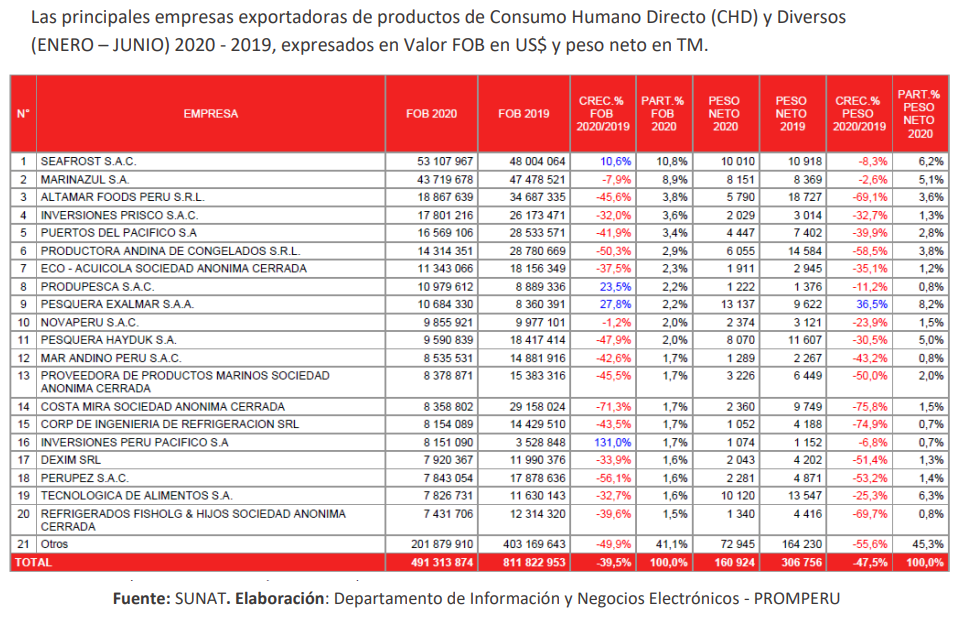
\includegraphics[keepaspectratio]{index_files/figure-html/lu137401d6rd_tmp_156be351.png}}

}

\end{figure}%

\subsection{Análisis del entorno}\label{anuxe1lisis-del-entorno}

\subsubsection{Externo: análisis PESTA}\label{externo-anuxe1lisis-pesta}

\begin{itemize}
\tightlist
\item
  \textbf{Factor político}
\end{itemize}

Estados Unidos vivirá un agitado año electoral. El crecimiento del
empleo y la estabilización de la economía serán sus principales cartas
de presentación de Donald Trump para ser reelegido; no obstante, el
aumento de la participación electoral de las minorías y de los jóvenes
le juega en contra.

\begin{itemize}
\tightlist
\item
  \textbf{Factor económico}
\end{itemize}

La COVID-19 (coronavirus) ha provocado la recesión mundial más profunda
que se ha experimentado en décadas. Si bien el resultado final aún es
incierto, debido a la pandemia la gran mayoría de los mercados
emergentes y de las economías en desarrollo se contraerá, con un daño
perdurable en la productividad laboral y el producto potencial. Una vez
que la crisis amaine, se deberá reafirmar un compromiso creíble con
políticas sostenibles y llevar a cabo las reformas que se necesiten para
apoyar las perspectivas a largo plazo. La coordinación y la cooperación
mundiales serán fundamentales. (Banco Mundial, 2020).

\begin{longtable}[]{@{}
  >{\raggedright\arraybackslash}p{(\linewidth - 14\tabcolsep) * \real{0.1250}}
  >{\centering\arraybackslash}p{(\linewidth - 14\tabcolsep) * \real{0.1250}}
  >{\centering\arraybackslash}p{(\linewidth - 14\tabcolsep) * \real{0.1250}}
  >{\centering\arraybackslash}p{(\linewidth - 14\tabcolsep) * \real{0.1250}}
  >{\centering\arraybackslash}p{(\linewidth - 14\tabcolsep) * \real{0.1250}}
  >{\centering\arraybackslash}p{(\linewidth - 14\tabcolsep) * \real{0.1250}}
  >{\centering\arraybackslash}p{(\linewidth - 14\tabcolsep) * \real{0.1250}}
  >{\centering\arraybackslash}p{(\linewidth - 14\tabcolsep) * \real{0.1250}}@{}}
\caption{Diferencia en puntos porcentuales con respecto a proyecciones
de enero 2020}\tabularnewline
\toprule\noalign{}
\begin{minipage}[b]{\linewidth}\raggedright
\end{minipage} & \begin{minipage}[b]{\linewidth}\centering
2017
\end{minipage} & \begin{minipage}[b]{\linewidth}\centering
2018
\end{minipage} & \begin{minipage}[b]{\linewidth}\centering
2019e
\end{minipage} & \begin{minipage}[b]{\linewidth}\centering
2020f
\end{minipage} & \begin{minipage}[b]{\linewidth}\centering
2021f
\end{minipage} & \begin{minipage}[b]{\linewidth}\centering
2020f
\end{minipage} & \begin{minipage}[b]{\linewidth}\centering
2021f
\end{minipage} \\
\midrule\noalign{}
\endfirsthead
\toprule\noalign{}
\begin{minipage}[b]{\linewidth}\raggedright
\end{minipage} & \begin{minipage}[b]{\linewidth}\centering
2017
\end{minipage} & \begin{minipage}[b]{\linewidth}\centering
2018
\end{minipage} & \begin{minipage}[b]{\linewidth}\centering
2019e
\end{minipage} & \begin{minipage}[b]{\linewidth}\centering
2020f
\end{minipage} & \begin{minipage}[b]{\linewidth}\centering
2021f
\end{minipage} & \begin{minipage}[b]{\linewidth}\centering
2020f
\end{minipage} & \begin{minipage}[b]{\linewidth}\centering
2021f
\end{minipage} \\
\midrule\noalign{}
\endhead
\bottomrule\noalign{}
\endlastfoot
\textbf{Mundo} & \textbf{3.3} & \textbf{3.0} & \textbf{2.4} &
\textbf{-5.2} & \textbf{4.2} & \textbf{-7.7} & \textbf{1.6} \\
Estados Unidos & 2.4 & 2.9 & 2.3 & -6.1 & 4.0 & -7.9 & 2.3 \\
Zona Euro & 2.5 & 1.9 & 1.2 & -9.1 & 4.5 & -10.1 & 3.2 \\
Japón & 2.2 & 0.3 & 0.7 & -6.1 & 2.5 & -6.8 & 1.9 \\
China & 6.8 & 6.6 & 6.1 & 1.0 & 6.9 & -4.9 & 1.1 \\
Federación de Rusia & 1.8 & 2.5 & 1.3 & -6.0 & 2.7 & -7.6 & 0.9 \\
\end{longtable}

\begin{itemize}
\tightlist
\item
  \textbf{Factor social}
\end{itemize}

Estados Unidos cuenta con una población proyectada par a el 2021 de
332,84 millones de habitantes la cual muestra un crecimiento de 0.77\%
considerando que la población en el presente año es de 331,05 millones
de habitantes, el 82\% de la población total es urbana la cual está
dispuesta siempre a probar nuevos productos de fácil consumo y sobre
todo que sean nutritivos.

\begin{itemize}
\tightlist
\item
  \textbf{Factor tecnológico}
\end{itemize}

La organización Mundial de la propiedad Intelectual (OMPI,2019), afirma
que Estados Unidos sigue siendo una de las naciones más innovadoras del
mundo.

\subsubsection{Interno: autodiagnóstico empresarial (análisis del
potencial
exportador)}\label{interno-autodiagnuxf3stico-empresarial-anuxe1lisis-del-potencial-exportador}

\begin{itemize}
\tightlist
\item
  \textbf{Gestión administrativa}
\end{itemize}

De acuerdo con el Sistema Integrado de Información de Comercio Exterior
(SIICEX,2019), las principales empresas peruanas exportadoras de trucha
frescas-refrigeradas, excepto hígados, huevas y lechas, en los períodos
2018, 2019 fueron Mar Andino Perú S.A.C. y Peruvian Andean Trout S.A.C.

Entre los principales mercados de exportación, Estados Unidos
experimenta una variación de -28\% de exportación entre los periodos
2018-2019, Japón, Uruguay y China experimentaron un aumento de 7629\%,
0\% y 2329\% mientras en Canadá disminuyó en -73\%; las ventas en
mercados como Estados Unidos para el 2019 tuvieron un valor de FOB
10,929.50 mil USD, seguido de Japón FOB 157.16 mil USD.

\begin{itemize}
\tightlist
\item
  \textbf{Gestión productiva y logística}
\end{itemize}

Se desarrollará la compra de truchas al por mayor de distintas partes de
la región dado que la región cuenta con la capacidad de producción
necesaria para abastecer el mercado tanto regional, nacional e
internacional.

\textbf{Capacidad.} La empresa contará con una amplia capacidad de
producción, utilizando el 100\% de su capacidad en abastecer el mercado
internacional.

\begin{itemize}
\tightlist
\item
  \textbf{Gestión económica y financiera}
\end{itemize}

De acuerdo al Plan Regional de Acuicultura de Ayacucho 2017-2021, en su
fase estratégica se indica un escenario positivo para el acceso a
créditos financieros, los cuales aumentarán para el año 2021 a 170
créditos a comparación con 2016 ya que se realizarán mayores charlas y
talleres informativos sobre los requisitos mínimos con los que debe
contar.

\subsection{Matriz FODA}\label{matriz-foda}

\subsubsection{Matriz de evaluación de los factores
internos}\label{matriz-de-evaluaciuxf3n-de-los-factores-internos}

La matriz cuenta con 15 factores determinantes de éxito, ocho fortalezas
y siete debilidades. La calificación ponderada, que se obtuvo para la
MEFI fue de 2.48; valor que se halla ligeramente por debajo del promedio
de la calificación que es de 2.5. Esto significa el sector acuicultura
presenta internamente cierto déficit que le impide competir con éxito
tanto en el mercado nacional e internacional, por lo tanto, debe ponerse
mayor atención a las debilidades, desarrollando estrategias internas
para superarlas.

\begin{figure}[H]

\caption{img}

{\centering \pandocbounded{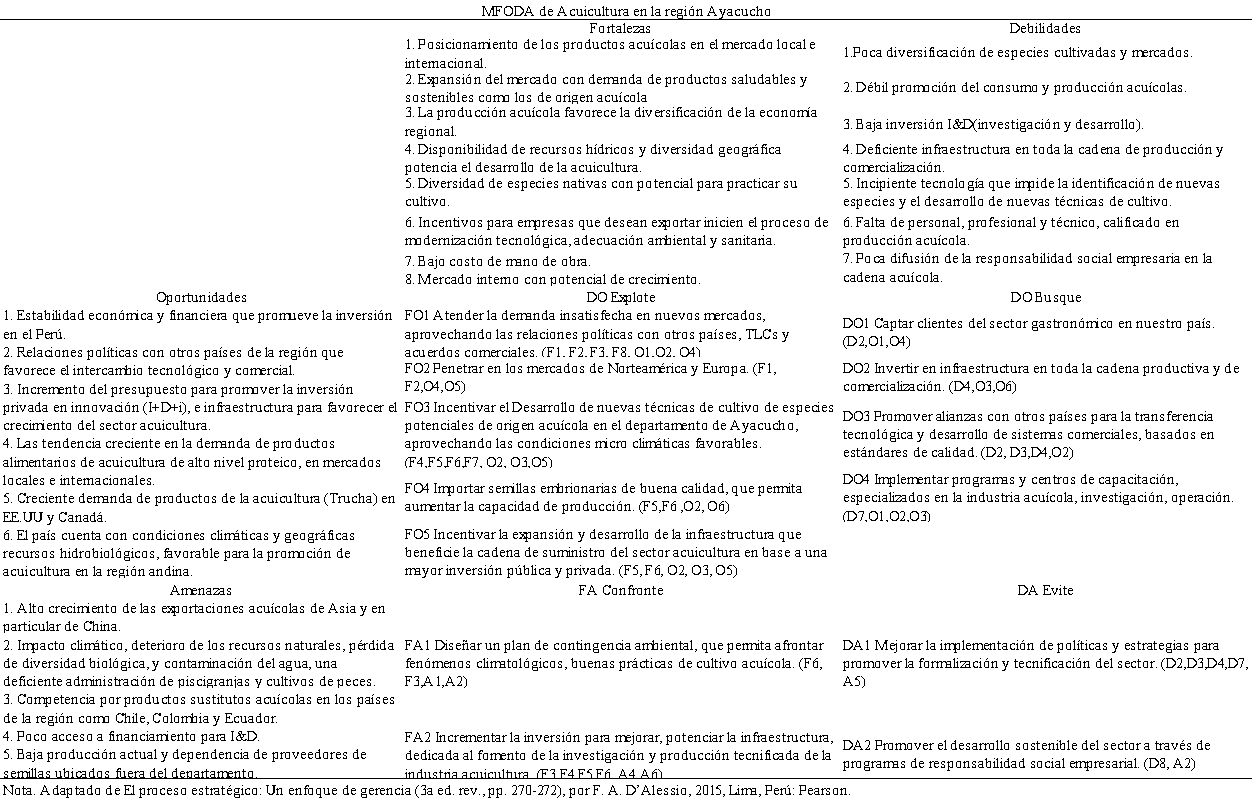
\includegraphics[keepaspectratio]{index_files/figure-html/lu137401d6rd_tmp_c6f73789.png}}

}

\end{figure}%

\textbf{Aplicación de la evaluación de los factores internos (Matriz
EFI)}

\begin{longtable}[]{@{}
  >{\raggedright\arraybackslash}p{(\linewidth - 6\tabcolsep) * \real{0.7000}}
  >{\centering\arraybackslash}p{(\linewidth - 6\tabcolsep) * \real{0.1000}}
  >{\centering\arraybackslash}p{(\linewidth - 6\tabcolsep) * \real{0.1000}}
  >{\centering\arraybackslash}p{(\linewidth - 6\tabcolsep) * \real{0.1000}}@{}}
\caption{Matriz de evaluación de los factores internos
(EFI)}\tabularnewline
\toprule\noalign{}
\begin{minipage}[b]{\linewidth}\raggedright
\textbf{Factores determinantes de éxito}
\end{minipage} & \begin{minipage}[b]{\linewidth}\centering
\textbf{Peso}
\end{minipage} & \begin{minipage}[b]{\linewidth}\centering
\textbf{Valor}
\end{minipage} & \begin{minipage}[b]{\linewidth}\centering
\textbf{Pond.}
\end{minipage} \\
\midrule\noalign{}
\endfirsthead
\toprule\noalign{}
\begin{minipage}[b]{\linewidth}\raggedright
\textbf{Factores determinantes de éxito}
\end{minipage} & \begin{minipage}[b]{\linewidth}\centering
\textbf{Peso}
\end{minipage} & \begin{minipage}[b]{\linewidth}\centering
\textbf{Valor}
\end{minipage} & \begin{minipage}[b]{\linewidth}\centering
\textbf{Pond.}
\end{minipage} \\
\midrule\noalign{}
\endhead
\bottomrule\noalign{}
\endlastfoot
\textbf{Fortalezas} & & & \\
Posicionamiento de los productos acuícolas en el mercado local e
internacional. & 0,08 & 4 & 0,32 \\
Expansión del mercado con demanda de productos saludables y sostenibles
como los de origen acuícola & 0,08 & 4 & 0,32 \\
La producción acuícola favorece la diversificación de la economía
regional & 0,07 & 3 & 0,21 \\
Disponibilidad de recursos hídricos y diversidad geográfica potencia el
desarrollo de acuicultura. & 0,09 & 4 & 0,36 \\
Diversidad de especies nativas con potencial para practicar su cultivo.
& 0,07 & 3 & 0,21 \\
Incentivos para empresas que desean exportar, inicien el proceso de
modernización tecnológica, adecuación ambiental y sanitaria. & 0,06 & 3
& 0,18 \\
Bajo costo de mano de obra. & 0,05 & 3 & 0,15 \\
Mercado interno con potencial de crecimiento. & 0,06 & 4 & 0,24 \\
\textbf{Subtotal fortalezas} & \textbf{0,56} & & \textbf{1,99} \\
\textbf{Debilidades} & & & \\
Poca diversificación de especies cultivadas y mercados. & 0,07 & 1 &
0,07 \\
Débil promoción del consumo y producción de productos acuícolas. & 0,05
& 2 & 0,1 \\
Baja inversión en I\&D & 0,04 & 1 & 0,04 \\
Deficiente infraestructura en toda la cadena de producción y
comercialización. & 0,06 & 2 & 0,12 \\
Incipiente tecnología que impide la identificación de nuevas especies y
el desarrollo de nuevas técnicas de cultivo. & 0,06 & 2 & 0,12 \\
Falta de personal, profesional y técnico, calificado en producción
acuícola & 0,07 & 1 & 0,07 \\
No existe difusión de la Responsabilidad Social Empresaria en la cadena
acuícola. & 0,09 & 1 & 0,09 \\
\textbf{Subtotal debilidades} & \textbf{0,44} & & \textbf{0,61} \\
\textbf{Total} & \textbf{1} & & \textbf{2,6} \\
\end{longtable}

De acuerdo con los resultados que arroja la matriz EFI observamos que la
empresa tiene una estructura interna muy débil puesto que al sumar todos
los criterios internos nos arroja un promedio de 2.6, lo que nos muestra
que está por encima de la suma promedio. Quiere decir que se está
planteando estrategias que ayuden a fortalecer la estructura interna de
la organización.

\subsubsection{Matriz de evaluación de los factores
externos}\label{matriz-de-evaluaciuxf3n-de-los-factores-externos}

Según se aprecia en la Tabla 2.4., en el análisis de la MEFE se obtuvo
como resultado 2.57, que es un valor mayor al promedio ponderado teórico
de 2.5 que significa la existencia de una ventaja relativa de las
fortalezas frente a las amenazas.

\textbf{Aplicación de evaluación de los factores externos (matriz EFE)}

\begin{longtable}[]{@{}
  >{\raggedright\arraybackslash}p{(\linewidth - 6\tabcolsep) * \real{0.7000}}
  >{\centering\arraybackslash}p{(\linewidth - 6\tabcolsep) * \real{0.1000}}
  >{\centering\arraybackslash}p{(\linewidth - 6\tabcolsep) * \real{0.1000}}
  >{\centering\arraybackslash}p{(\linewidth - 6\tabcolsep) * \real{0.1000}}@{}}
\caption{Matriz de evaluación de los factores externos}\tabularnewline
\toprule\noalign{}
\begin{minipage}[b]{\linewidth}\raggedright
\textbf{Factores determinantes de éxito}
\end{minipage} & \begin{minipage}[b]{\linewidth}\centering
\textbf{Peso}
\end{minipage} & \begin{minipage}[b]{\linewidth}\centering
\textbf{Valor}
\end{minipage} & \begin{minipage}[b]{\linewidth}\centering
\textbf{Pond.}
\end{minipage} \\
\midrule\noalign{}
\endfirsthead
\toprule\noalign{}
\begin{minipage}[b]{\linewidth}\raggedright
\textbf{Factores determinantes de éxito}
\end{minipage} & \begin{minipage}[b]{\linewidth}\centering
\textbf{Peso}
\end{minipage} & \begin{minipage}[b]{\linewidth}\centering
\textbf{Valor}
\end{minipage} & \begin{minipage}[b]{\linewidth}\centering
\textbf{Pond.}
\end{minipage} \\
\midrule\noalign{}
\endhead
\bottomrule\noalign{}
\endlastfoot
\textbf{Fortalezas} & & & \\
Posicionamiento de los productos acuícolas en el mercado local e
internacional. & 0,08 & 4 & 0,32 \\
Expansión del mercado con demanda de productos saludables y sostenibles
como los de origen acuícola & 0,08 & 4 & 0,32 \\
La producción acuícola favorece la diversificación de la economía
regional & 0,07 & 3 & 0,21 \\
Disponibilidad de recursos hídricos y diversidad geográfica potencia el
desarrollo de acuicultura. & 0,09 & 4 & 0,36 \\
Diversidad de especies nativas con potencial para practicar su cultivo.
& 0,07 & 3 & 0,21 \\
Incentivos para empresas que desean exportar, inicien el proceso de
modernización tecnológica, adecuación ambiental y sanitaria. & 0,06 & 3
& 0,18 \\
Bajo costo de mano de obra. & 0,05 & 3 & 0,15 \\
Mercado interno con potencial de crecimiento. & 0,06 & 4 & 0,24 \\
\textbf{Subtotal fortalezas} & \textbf{0,56} & & \textbf{1,99} \\
\textbf{Debilidades} & & & \\
Poca diversificación de especies cultivadas y mercados. & 0,07 & 1 &
0,07 \\
Débil promoción del consumo y producción de productos acuícolas. & 0,05
& 2 & 0,1 \\
Baja inversión en I\&D & 0,04 & 1 & 0,04 \\
Deficiente infraestructura en toda la cadena de producción y
comercialización. & 0,06 & 2 & 0,12 \\
Incipiente tecnología que impide la identificación de nuevas especies y
el desarrollo de nuevas técnicas de cultivo. & 0,06 & 2 & 0,12 \\
Falta de personal, profesional y técnico, calificado en producción
acuícola & 0,07 & 1 & 0,07 \\
No existe difusión de la Responsabilidad Social Empresaria en la cadena
acuícola. & 0,09 & 1 & 0,09 \\
\textbf{Subtotal debilidades} & \textbf{0,44} & & \textbf{0,61} \\
\textbf{Total} & \textbf{1} & & \textbf{2,6} \\
\end{longtable}

\subsection{Plan estratégico}\label{plan-estratuxe9gico}

Se muestran las estrategias, los intereses de la organización, las
políticas, los principios, los valores de la organización, código de
ética, tablero de control, y que cada uno esté vinculado o relacionado
con la visión y misión organizacional, esta herramienta permite también
tomar decisiones, toda vez que en el desarrollo del plan en el tiempo
surgen situaciones externas e internas que conllevan a realizar ajustes
y cambios, sobre todo en las estrategias planteadas. La industria de la
acuicultura está en la etapa de formación y desarrollo, por lo que los
cambios y ajustes a las estrategias, así como en los objetos de corto
plazo se continuarán dando, junto con la permanente innovación
tecnológica y científica que se viene desarrollando a nivel global en
este sector.

\subsubsection{Visión}\label{visiuxf3n}

Para el año 2022, la región del Ayacucho será el tercer productor de
especies acuícolas y logrará comercializar con mercados internacionales
como el de Estados Unidos, Japón, Canadá, Europa, debido a la ventaja
comparativa con la que cuenta, con una cadena productiva que elevará su
competitividad, con altos estándares de calidad, con una oferta
exportable durante todo el año y promoviendo el crecimiento y bienestar
de la comunidad vinculada, cumpliendo los estándares de calidad
requeridos, contribuyendo al cuidado del medio ambiente.

\subsubsection{Misión}\label{misiuxf3n}

Producir y exportar la Trucha Arcoíris, para el consumo humano a los
mercados locales como también internacionales tales como Estados Unidos,
Japón, Canadá y parte de la Comunidad Europea, garantizando una
alimentación sana y nutritiva científica, utilizando los últimos avances
tecnológicos, e innovación creativa y de calidad, en toda la cadena
productiva de la acuicultura regional y poder lograr un crecimiento
rentable y sostenible, aprovechando las ventajas geográficas y de
biodiversidad de la región Ayacucho.

\subsection{Objetivos específicos - estrategias e
indicadores}\label{objetivos-especuxedficos---estrategias-e-indicadores}

\subsubsection{Objetivos específicos}\label{objetivos-especuxedficos}

\begin{longtable}[]{@{}
  >{\raggedright\arraybackslash}p{(\linewidth - 4\tabcolsep) * \real{0.2603}}
  >{\raggedright\arraybackslash}p{(\linewidth - 4\tabcolsep) * \real{0.4795}}
  >{\raggedright\arraybackslash}p{(\linewidth - 4\tabcolsep) * \real{0.2603}}@{}}
\caption{Tabla de objetivos, estrategias e indicadores.}\tabularnewline
\toprule\noalign{}
\begin{minipage}[b]{\linewidth}\raggedright
OBJETIVOS ESPECÍFICOS
\end{minipage} & \begin{minipage}[b]{\linewidth}\raggedright
ESTRATEGIA
\end{minipage} & \begin{minipage}[b]{\linewidth}\raggedright
INDICADOR
\end{minipage} \\
\midrule\noalign{}
\endfirsthead
\toprule\noalign{}
\begin{minipage}[b]{\linewidth}\raggedright
OBJETIVOS ESPECÍFICOS
\end{minipage} & \begin{minipage}[b]{\linewidth}\raggedright
ESTRATEGIA
\end{minipage} & \begin{minipage}[b]{\linewidth}\raggedright
INDICADOR
\end{minipage} \\
\midrule\noalign{}
\endhead
\bottomrule\noalign{}
\endlastfoot
OEE1. Captar clientes en EE. UU & Elaborar un plan de Marketing digital
y posicionar nuestra marca dentro de las redes sociales, revistas
virtuales y realizar publicidades en medios estadounidenses. & Número de
clientes en EE. UU \\
OEE2. Incrementar contactos con potenciales importadores & Participar de
ferias internacionales donde se dé a conocer el producto & Número de
participaciones en ferias \\
OEE3. Crear alianzas estratégicas con proveedores & Contactar a los
proveedores de materia prima y establecer relaciones & Número de
proveedores contactados \\
OEE4. Ofrecer productos de calidad & Establecer una producción bajo los
estándares de calidad internacional y participar en diferentes
conferencias que ayuden a mejorar la calidad de nuestro producto &
Números de certificaciones \\
OEE5. Hacer conocer nuestro producto como saludable y ecológico &
Realizar una campaña de publicidad acerca de los beneficios de nuestro
producto y resaltarlos en el etiquetado de este. & \% de compradores que
prefieren nuestro producto \\
\end{longtable}

\subsection{Plan organizacional}\label{plan-organizacional}

\subsubsection{Organigrama}\label{organigrama}

\begin{figure}[H]

\caption{Organigrama de la empresa AQUAZUL}

{\centering \pandocbounded{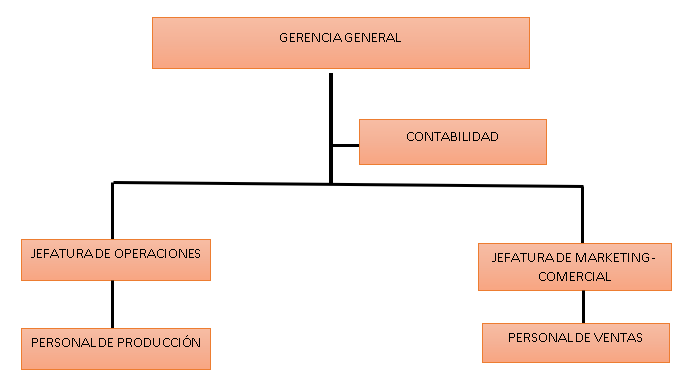
\includegraphics[keepaspectratio]{index_files/figure-html/lu137401d6rd_tmp_eddade33.png}}

}

\end{figure}%

\begin{enumerate}
\def\labelenumi{\alph{enumi})}
\tightlist
\item
  \textbf{Área: Gerencia general}
\end{enumerate}

\textbf{Gerente General:} Será el que representa, imagen y encargado de
administrar el funcionamiento y desarrollo de manera eficiente la
empresa.

\begin{enumerate}
\def\labelenumi{\alph{enumi})}
\setcounter{enumi}{1}
\tightlist
\item
  \textbf{Área: Contabilidad}
\end{enumerate}

\textbf{Contador:} Dirigir las operaciones relacionadas con la
Contabilidad General y planificar actividades necesarias para el cierre
oportuno de la información contable.

\begin{enumerate}
\def\labelenumi{\alph{enumi})}
\setcounter{enumi}{2}
\tightlist
\item
  \textbf{Área: Departamento de operaciones}
\end{enumerate}

\textbf{Jefe de operaciones:} Será quien se encargue de liderazgo en la
gestión tanto de las materias primas y como del personal de operaciones.
La supervisión del inventario, de las compras y los suministros es
fundamental para el trabajo. Asimismo, elaboración de presupuestos,
control de costos y el mantenimiento de la organización.

\textbf{Personal de producción:} Personal encargado de la empaquetar,
embalar y verificar la etapa final de la producción para que el producto
esté en condiciones de comercializarse.

\begin{enumerate}
\def\labelenumi{\alph{enumi})}
\setcounter{enumi}{3}
\tightlist
\item
  \textbf{Área: Departamento de marketing y comercialización.}
\end{enumerate}

\textbf{Cargo: jefe de marketing y comercialización}

Esta persona tendrá que trabajar con bastante innovación porque debe
lograr eliminar la estacionalidad del producto, hacerlo conocido y con
ello generar ventas. Estará encargado de la administración de los puntos
de venta presencial y online.

\textbf{Personal de Ventas}: Personal encargado de mantener un trato
directo con el cliente realiza las ventas del producto en los canales de
ventas.

\subsection{Plan de recursos humanos}\label{plan-de-recursos-humanos}

\subsubsection{Tipos de reclutamiento}\label{tipos-de-reclutamiento}

\begin{itemize}
\tightlist
\item
  \hspace{0pt} \textbf{Reclutamiento interno:} Se desarrollará un
  programa de desarrollo personal para los empleados, procesamiento y
  exportación de truchas.
\item
  \textbf{\hspace{0pt} Reclutamiento externo:} El reclutamiento externo
  de personal se realizará de dos formas, el primero será mediante el
  uso de agencias de reclutamiento y la segunda forma será mediante
  carteles públicos u avisos en los periódicos.
\end{itemize}

\subsubsection{Tipos de selección}\label{tipos-de-selecciuxf3n}

\begin{itemize}
\tightlist
\item
  \hspace{0pt} Se realizará una entrevista de trabajo con prueba de
  conocimiento específico, porque creemos que la especialización es de
  primordial importancia para el mejor desenvolvimiento de las labores.
\item
  \hspace{0pt} Por último, para considerar que el postulante es apto
  para el puesto al que aspira se tomara una prueba psicotécnica de
  aptitud, esto para medir las habilidades, competencias y capacidad del
  postulante.
\end{itemize}

\subsubsection{Tipos de inducción}\label{tipos-de-inducciuxf3n}

En la inducción el jefe de sección será el encargado de dar la
bienvenida al nuevo empleado, de mostrarle cual es proceso de producción
general en la empresa e indicarle cuál es su labor especifica.

\subsubsection{Tipos de capacitación}\label{tipos-de-capacitaciuxf3n}

La capacitación en la empresa será mediante una planeación de
actividades de trabajo, es decir cursos de capacitación programadas.

\subsection{Cronograma de actividades}\label{cronograma-de-actividades}

\begin{figure}[H]

\caption{Cronograma de actividades de la empresa AQUAZUL.}

{\centering \pandocbounded{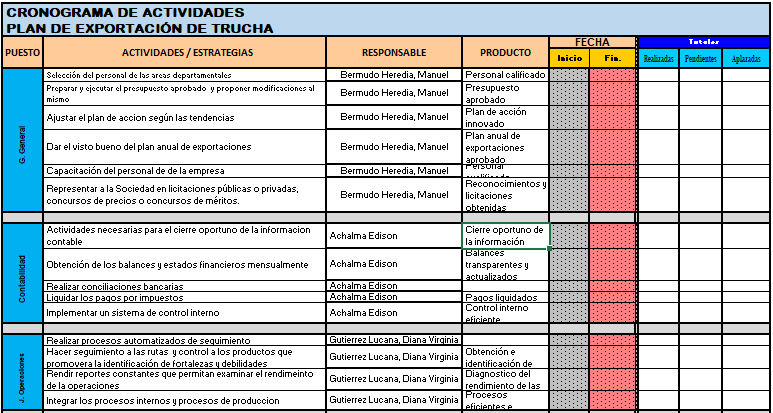
\includegraphics[keepaspectratio]{index_files/figure-html/lu137401d6rd_tmp_20cc7e3e.png}}

}

\end{figure}%

\section{Capítulo III Estudio de mercado internacional y plan de
marketing}\label{capuxedtulo-iii-estudio-de-mercado-internacional-y-plan-de-marketing}

\subsection{Estudio de mercado
internacional}\label{estudio-de-mercado-internacional}

\begin{figure}[!htbp]

{\caption{{Mercado mundial de salmónidos 2017-2022 (Miles de
toneladas)}{\label{fig-myimportedimage}}}}

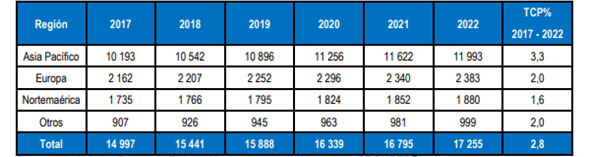
\includegraphics[width=5in,height=\textheight,keepaspectratio]{index_files/figure-html/lu137401d6rd_tmp_71aa4fe1.png}

{\noindent \emph{Note.} Inteligencia de Mercados-PROMPERU, 2018}

\end{figure}

El gráfico muestra al mercado norteamericano al cuál irá dirigido
nuestro producto presenta un incremento a nivel del consumo de esta
especie, lo cual es un escenario bastante favorable. En los últimos
años, los consumidores norteamericanos de mayores ingresos buscan pagar
más por presentaciones frescas debido a que son percibidas como más
``naturales'' y ``saludables''.

\subsection{Descripción del
producto}\label{descripciuxf3n-del-producto-1}

\textbf{Características del producto}

La trucha es un alimento muy nutritivo rico en energía, agua, proteínas,
grasas, carbohidratos, calcio, fósforo, hierro. La partida arancelaria
es 0304420000.

\begin{figure}[H]

\caption{Principales subpartidas arancelarias para las truchas Arcoíris}

{\centering \pandocbounded{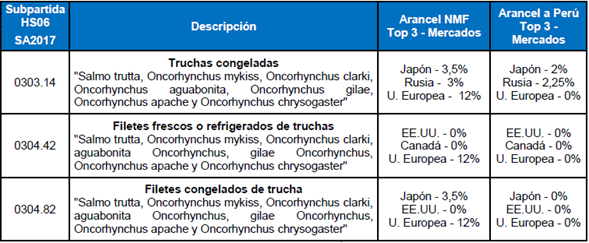
\includegraphics[keepaspectratio]{index_files/figure-html/lu137401d6rd_tmp_591778ab.png}}

}

\end{figure}%

\textbf{Formas de Presentación:} Filete de trucha fresca en pack de 1Kg.

\textbf{Zona de Producción:} Ayacucho

\textbf{Usos:} Para el consumo humano.

\textbf{Principales Mercados:} Estados Unidos, Japón, Canadá.

\subsection{Identificación del
problema}\label{identificaciuxf3n-del-problema}

\textbf{Objetivo general}

Posicionar nuestro producto con los estándares de calidad a nivel
mundial, en el mercado estadounidense.

\subsection{Análisis del producto y cartera de
productos}\label{anuxe1lisis-del-producto-y-cartera-de-productos}

\textbf{Ciclo de vida del producto}

\begin{figure}[H]

\caption{Evolución de las exportaciones peruanas de trucha por
presentaciones}

{\centering \pandocbounded{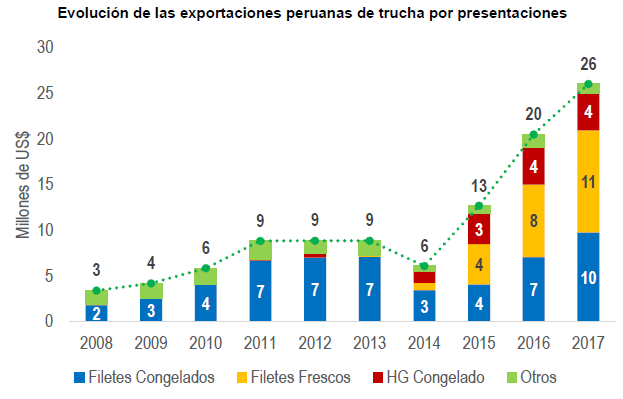
\includegraphics[keepaspectratio]{index_files/figure-html/lu137401d6rd_tmp_f38016ab.png}}

}

\end{figure}%

\subsection{Selección del mercado
objetivo}\label{selecciuxf3n-del-mercado-objetivo}

\begin{longtable}[]{@{}
  >{\raggedright\arraybackslash}p{(\linewidth - 6\tabcolsep) * \real{0.7000}}
  >{\centering\arraybackslash}p{(\linewidth - 6\tabcolsep) * \real{0.1000}}
  >{\centering\arraybackslash}p{(\linewidth - 6\tabcolsep) * \real{0.1000}}
  >{\centering\arraybackslash}p{(\linewidth - 6\tabcolsep) * \real{0.1000}}@{}}
\caption{Canales de distribución y logística exportadora}\tabularnewline
\toprule\noalign{}
\begin{minipage}[b]{\linewidth}\raggedright
\textbf{Canales de distribución y logística exportadora}
\end{minipage} & \begin{minipage}[b]{\linewidth}\centering
\textbf{EE.UU}
\end{minipage} & \begin{minipage}[b]{\linewidth}\centering
\textbf{Japón}
\end{minipage} & \begin{minipage}[b]{\linewidth}\centering
\textbf{Canadá}
\end{minipage} \\
\midrule\noalign{}
\endfirsthead
\toprule\noalign{}
\begin{minipage}[b]{\linewidth}\raggedright
\textbf{Canales de distribución y logística exportadora}
\end{minipage} & \begin{minipage}[b]{\linewidth}\centering
\textbf{EE.UU}
\end{minipage} & \begin{minipage}[b]{\linewidth}\centering
\textbf{Japón}
\end{minipage} & \begin{minipage}[b]{\linewidth}\centering
\textbf{Canadá}
\end{minipage} \\
\midrule\noalign{}
\endhead
\bottomrule\noalign{}
\endlastfoot
El conocimiento de los canales de distribución en el país objetivo es
amplio & 3 & 3 & 3 \\
Los medios logísticos existentes permiten llegar sin mayor retraso o
dificultad a este mercado & 3 & 3 & 3 \\
Los costos de transporte no afectan significativamente las posibilidades
de exportación de mi producto & 2 & 2 & 2 \\
Los requerimientos de envase y embalaje del país de destino no
constituyen una dificultad a la exportación & 3 & 2 & 3 \\
Poseo suficientes experiencias en contratos de compra venta
internacional y conocimiento de condiciones de pago más frecuentes en el
país objetivo & 1 & 1 & 1 \\
\end{longtable}

\begin{table}

{\caption{{Medición de la intensidad de la
competencia}{\label{tbl-mytable}}}}

\begin{longtable}[]{@{}
  >{\raggedright\arraybackslash}p{(\linewidth - 6\tabcolsep) * \real{0.5500}}
  >{\centering\arraybackslash}p{(\linewidth - 6\tabcolsep) * \real{0.1500}}
  >{\centering\arraybackslash}p{(\linewidth - 6\tabcolsep) * \real{0.1500}}
  >{\centering\arraybackslash}p{(\linewidth - 6\tabcolsep) * \real{0.1500}}@{}}
\toprule\noalign{}
\begin{minipage}[b]{\linewidth}\raggedright
\textbf{Intensidad de la competencia}
\end{minipage} & \begin{minipage}[b]{\linewidth}\centering
\textbf{EE.UU}
\end{minipage} & \begin{minipage}[b]{\linewidth}\centering
\textbf{Japón}
\end{minipage} & \begin{minipage}[b]{\linewidth}\centering
\textbf{Canadá}
\end{minipage} \\
\midrule\noalign{}
\endhead
\bottomrule\noalign{}
\endlastfoot
Los productores locales no representan una fuerte competencia y no
tienen una gran capacidad de influencia sobre las políticas comerciales
& 2 & 2 & 2 \\
Los competidores externos son pocos y presentan un bajo posicionamiento
en el mercado & 3 & 3 & 1 \\
Los exportadores peruanos de mis productos son escasos y no presentan en
la actualidad un posicionamiento superior al de mi empresa en este
mercado & 3 & 3 & 3 \\
\textbf{Total} & \textbf{8} & \textbf{8} & \textbf{6} \\
\end{longtable}

{\noindent \emph{Note.} No/Nunca = 1; Algunos/A veces = 2; Si/Siempre = 3}

\end{table}

\begin{table}

{\caption{{Medición de riesgo}{\label{tbl-mytable}}}}

\begin{longtable}[]{@{}
  >{\raggedright\arraybackslash}p{(\linewidth - 6\tabcolsep) * \real{0.3014}}
  >{\centering\arraybackslash}p{(\linewidth - 6\tabcolsep) * \real{0.2329}}
  >{\centering\arraybackslash}p{(\linewidth - 6\tabcolsep) * \real{0.2329}}
  >{\centering\arraybackslash}p{(\linewidth - 6\tabcolsep) * \real{0.2329}}@{}}
\toprule\noalign{}
\begin{minipage}[b]{\linewidth}\raggedright
\textbf{Riesgos}
\end{minipage} & \begin{minipage}[b]{\linewidth}\centering
\textbf{EE.UU}
\end{minipage} & \begin{minipage}[b]{\linewidth}\centering
\textbf{Japón}
\end{minipage} & \begin{minipage}[b]{\linewidth}\centering
\textbf{Canadá}
\end{minipage} \\
\midrule\noalign{}
\endhead
\bottomrule\noalign{}
\endlastfoot
El país no presenta riesgos desde el punto de vista socioeconómico,
político legal y comercial. & 3 & 3 & 3 \\
Las empresas con las que voy a negociar presentan un nivel de riesgo
entre bajo y mínimo & 3 & 3 & 3 \\
La percepción de la comunidad empresarial respecto a la calidad de buen
pagador de las empresas del país es buena & 3 & 3 & 3 \\
\textbf{Total} & \textbf{9} & \textbf{9} & \textbf{9} \\
\end{longtable}

{\noindent \emph{Note.} No/Nunca = 1; Algunos/A veces = 2; Si/Siempre = 3}

\end{table}

\begin{table}

{\caption{{Medición de la distancia sicológica}{\label{tbl-mytable}}}}

\begin{longtable}[]{@{}
  >{\raggedright\arraybackslash}p{(\linewidth - 6\tabcolsep) * \real{0.3014}}
  >{\centering\arraybackslash}p{(\linewidth - 6\tabcolsep) * \real{0.2329}}
  >{\centering\arraybackslash}p{(\linewidth - 6\tabcolsep) * \real{0.2329}}
  >{\centering\arraybackslash}p{(\linewidth - 6\tabcolsep) * \real{0.2329}}@{}}
\toprule\noalign{}
\begin{minipage}[b]{\linewidth}\raggedright
\textbf{Distancia Sicológica}
\end{minipage} & \begin{minipage}[b]{\linewidth}\centering
\textbf{EE.UU}
\end{minipage} & \begin{minipage}[b]{\linewidth}\centering
\textbf{Japón}
\end{minipage} & \begin{minipage}[b]{\linewidth}\centering
\textbf{Canadá}
\end{minipage} \\
\midrule\noalign{}
\endhead
\bottomrule\noalign{}
\endlastfoot
mi empresa tiene experiencia en el mercado & 1 & 1 & 1 \\
Existe afinidad cultural y buena comunicación con la comunidad
empresarial de este país & 3 & 2 & 3 \\
mi empresa cuanta con contactos de negocios previamente establecidos & 2
& 2 & 2 \\
Mi producto puede ser adaptado a los requerimientos del mercado, de ser
necesario, sin mayor dificultad & 3 & 2 & 3 \\
\textbf{Total} & \textbf{9} & \textbf{7} & \textbf{9} \\
\end{longtable}

{\noindent \emph{Note.} No/Nunca = 1; Algunos/A veces = 2; Si/Siempre = 3}

\end{table}

\begin{figure}[H]

\caption{Países ofertantes de trucha en el mercado internacional}

{\centering \pandocbounded{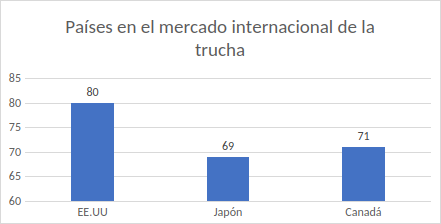
\includegraphics[keepaspectratio]{index_files/figure-html/image-20250326090505942.png}}

}

\end{figure}%

En el gráfico se puede apreciar que acorde al test, es recomendable
realizar el análisis de la oferta y la Demanda en el país de EE. UU, que
obtuvo 80 puntos, respecto a Canadá y Japón los cuales obtuvieron
puntajes menores.

\subsection{Análisis de la oferta}\label{anuxe1lisis-de-la-oferta}

TRADEMAP afirma que Estados Unidos exporta filete de trucha teniendo
como principal proveedor el mercado de Chile, con una participación en
el año 2017 del 59\%; Noruega con 34\%; Canadá 4\%; Colombia 0.9 \%.
SUNAT afirma que en el año 2017 Perú exportó filete de trucha a Estados
Unidos bajo la partida arancelaria 0304422 con un valor FOB de \$ 11,
086,417, lo que muestra un crecimiento del 42\% con respecto al año
2016. Siendo el principal productor de trucha en el Perú es Mar Andino
Perú S.A.C. y Peruvian Andean Trout S.A.C.

\subsubsection{Análisis de la competencia
internacional}\label{anuxe1lisis-de-la-competencia-internacional}

\begin{figure}[H]

\caption{Principales Exportadores de Filetes de Trucha Congelada del
mundo}

{\centering \pandocbounded{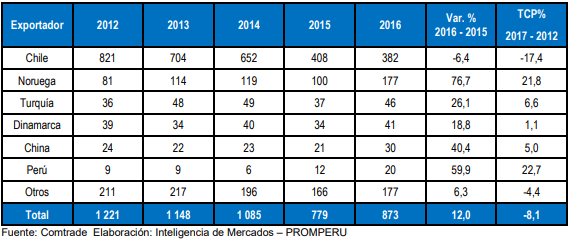
\includegraphics[keepaspectratio]{index_files/figure-html/lu137401d6rd_tmp_e9a2665f.png}}

}

\end{figure}%

\textbf{Perú:} nuestro país ocupa el sexto lugar entre los principales
exportadores de trucha congelada.

El gráfico anterior nos muestra una oportunidad acerca de la exportación
de trucha al mercado estadounidense pues como se ve, ninguno de los
principales exportadores de trucha destina su producto a este mercado,
lo cual representa una gran oportunidad para nosotros.

\subsection{Mercado objetivo}\label{mercado-objetivo}

Al aplicar el test de selección el país que obtuvo el mayor puntaje es
EE.UU, dado que este cuenta con las características como por ejemplo
tratados de libre comercio que lo convierten en un mercado más accesible
para realizar un comercio , por lo tanto de aquí en adelante se
realizara todos los estudios respectivos para conocer las
características de los consumidores estadounidenses con respecto al
filete de trucha arcoíris por ello todos los esfuerzos están abocados a
este mercado como acciones a tomar, certificaciones , estrategias de
negociación que se van a utilizar para una óptima negociación en este
mercado.

\subsection{Ficha país}\label{ficha-pauxeds}

\begin{table}

{\caption{{Ficha país de Estados Unidos de
Norteamérica}{\label{tbl-mytable}}}}

\begin{longtable}[]{@{}
  >{\raggedright\arraybackslash}p{(\linewidth - 2\tabcolsep) * \real{0.2917}}
  >{\raggedright\arraybackslash}p{(\linewidth - 2\tabcolsep) * \real{0.7083}}@{}}
\toprule\noalign{}
\begin{minipage}[b]{\linewidth}\raggedright
\end{minipage} & \begin{minipage}[b]{\linewidth}\raggedright
FICHA PAÍS: ESTADOS UNIDOS DE AMÉRICA
\end{minipage} \\
\midrule\noalign{}
\endhead
\bottomrule\noalign{}
\endlastfoot
\textbf{Área:} & 9 826 675 km2 \\
\textbf{Capital:} & Washington D.C \\
\textbf{Ciudades importantes:} & 18.804 millones Nueva York-Newark,
12.447 millones Los Ángeles-Long Beach-Santa Ana, 8.865 millones
Chicago, 6.371 millones Houston, 6.301 millones Dallas-Fort Worth, 5.322
millones WASHINGTON, DC (capital) (2020) \\
\textbf{Población:} & 329,278 864 \\
\textbf{Idioma oficial:} & No tiene idioma oficial, pero el inglés ha
adquirido status oficial en 31 de los 50 estados. \\
\textbf{Ubicación geográfica} & Norte América, bordea el Norte de los
Océanos Atlántico y Pacifico, entre Canadá y México. \\
\textbf{Organización territorial:} & 50 estados y 1 distrito. \\
\textbf{PBI:} & \$ 19,49 billones (2019) \\
\textbf{PBI per cápita:} & \$ 59.800 (2019) \\
\textbf{Tasa de crecimiento anual:} & 0,72\% (2019) \\
\textbf{Moneda:} & Dólar estadounidense \\
\textbf{Clima:} & Es muy variado, depende de la estación y de la
ubicación. \\
\textbf{Voltaje:} & 110 voltios \\
\textbf{Pesos y medidas:} & Libras, onzas, pulgadas, yardas, millas. \\
\textbf{Días festivos:} & 1 de enero, 20 de enero, 17 de febrero, 31 de
marzo, 5 de mayo, 26 de mayo, 4 de julio, 1 de setiembre, 13 de octubre,
11 de noviembre, 27 de noviembre y 25 de diciembre. \\
\textbf{Códigos telefónicos:} & 00 + 1 + Ciudad + Número \\
\end{longtable}

{\noindent \emph{Note.} The World Fatbook-CIA}

\end{table}

\subsection{Exigencias del producto}\label{exigencias-del-producto}

\begin{table}

{\caption{{Exigencias del producto a exportar}{\label{tbl-mytable}}}}

\begin{longtable}[]{@{}
  >{\raggedright\arraybackslash}p{(\linewidth - 2\tabcolsep) * \real{0.3333}}
  >{\raggedright\arraybackslash}p{(\linewidth - 2\tabcolsep) * \real{0.6667}}@{}}
\toprule\noalign{}
\begin{minipage}[b]{\linewidth}\raggedright
\textbf{Exigencia del producto:}
\end{minipage} & \begin{minipage}[b]{\linewidth}\raggedright
Filete de trucha
\end{minipage} \\
\midrule\noalign{}
\endhead
\bottomrule\noalign{}
\endlastfoot
\textbf{En el mercado de:} & Estados Unidos de América. \\
\textbf{Acuerdos comerciales- Arancel- Preferencias arancelarias} &
Estados unidos otorga preferencia arancelaria con un arancel del 0\%,
Por el tratado de libre comercio EE. UU-Perú. El Acuerdo de Promoción
Comercial (APC) Perú -- EE. UU. \\
\textbf{Denominación de origen:} & No cuenta con denominación de
origen. \\
\textbf{Normas de empaque:} & Se aplicará la ley sobre etiquetado de
productos nutritivos y educación (NLEA) \\
\end{longtable}

{\noindent \emph{Note.} Ministerio de Comercio Exterior y Turismo (2019), Ministerio de La Producción (2019), FDA.}

\end{table}

\subsubsection{Barreras arancelarias}\label{barreras-arancelarias}

Perú por el tratado de libre comercio firmado con el país de Estados
Unidos tiene un arancel del 0\% para nuestro producto a exportar bajo la
partida arancelaria 0304420000, lo cual es muy beneficioso para
comercializar con este país.

\subsubsection{Barreras pararancelarias}\label{barreras-pararancelarias}

No existen barreras pararancelarias que impidan o compliquen la
exportación de trucha a Estados Unidos de América.

\subsection{Canales de distribución}\label{canales-de-distribuciuxf3n}

\textbf{Forma de distribución:}

Los componentes principales en la distribución del producto serán los
siguientes:

\begin{longtable}[]{@{}
  >{\raggedright\arraybackslash}p{(\linewidth - 2\tabcolsep) * \real{0.2917}}
  >{\raggedright\arraybackslash}p{(\linewidth - 2\tabcolsep) * \real{0.7083}}@{}}
\caption{Composición y descripción de los actores de la cadena
distributiva}\tabularnewline
\toprule\noalign{}
\begin{minipage}[b]{\linewidth}\raggedright
COMPONENTE
\end{minipage} & \begin{minipage}[b]{\linewidth}\raggedright
DESCRIPCIÓN
\end{minipage} \\
\midrule\noalign{}
\endfirsthead
\toprule\noalign{}
\begin{minipage}[b]{\linewidth}\raggedright
COMPONENTE
\end{minipage} & \begin{minipage}[b]{\linewidth}\raggedright
DESCRIPCIÓN
\end{minipage} \\
\midrule\noalign{}
\endhead
\bottomrule\noalign{}
\endlastfoot
Exportador & Dueño del producto de la empresa exportadora, en este caso
es la empresa exportadora de trucha fresca y congelada Aquazul. \\
Distribuidor a mayorista & El exportador seguirá siendo responsable por
los defectos o daños causados por los productos, pero el distribuidor
será responsable ante la aduana y en general ante las autoridades
americanas una vez que la mercancía haya sido nacionalizada. La empresa
o el supermercado mayorista será New Atlantic S.A.C. \\
Detallista o minorista & Serán los minimarkets estadounidenses, este se
encargará de la compra de mercancías para su reventa y la exhibición de
la misma. Adquirirá los productos directamente a la empresa
distribuidora New Atlantic S.A.C. \\
Usuario o consumidor final & La persona final de la cadena de
distribución serán las familias estadounidenses de aquellos lugares
donde New Atlantic S.A.C. tenga sucursales. \\
\end{longtable}

El canal de distribución de la empresa Aquazul será por medio del
\emph{canal mayorista o canal cuatro} ya que la trucha ira del
productor, a manos del mayorista o distribuidor, luego pasará por un
minorista o detallista para llegar al consumidor final o usuario, de la
siguiente forma:

Exportador---------\textgreater{} Distribuidor--------\textgreater{}
Minorista---------\textgreater{} Usuario

\begin{figure}[H]

\caption{Proceso de producción}

{\centering \pandocbounded{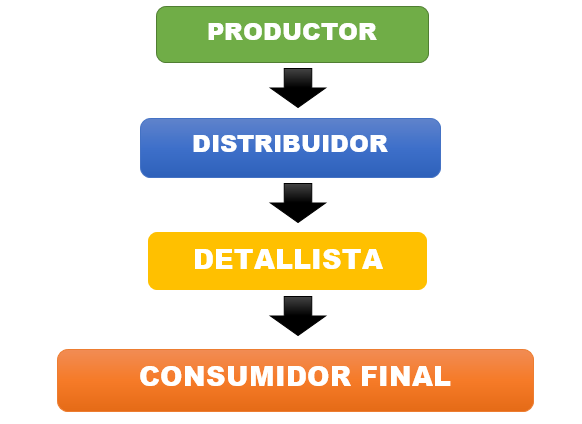
\includegraphics[keepaspectratio]{index_files/figure-html/lu137401d6rd_tmp_52655096.png}}

}

\end{figure}%%
\begin{figure}[H]

\caption{Canal de distribución}

{\centering \pandocbounded{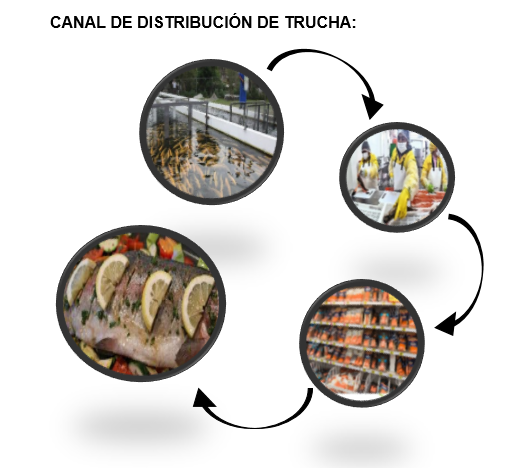
\includegraphics[keepaspectratio]{index_files/figure-html/lu137401d6rd_tmp_d9c46710.png}}

}

\end{figure}%

En el gráfico se muestra como la trucha arcoíris será producida por las
empresas asociadas a la empresa Aquazul, pasarán por un proceso en el
que se le dará un mayor valor agregado al convertirlo en filetes y
llegará a manos de la empresa mayorista (supermercado Trader Joe´s)

\subsection{Medio de transporte}\label{medio-de-transporte}

\textbf{Transporte aéreo de mercancías:}

El medio de transporte utilizado para los envíos de la empresa Aquazul
será el aéreo, se escogió este medio debido a su rapidez, seguridad,
facilidad, control, seguimiento y principalmente por que la trucha es un
producto delicado y perecedero.

El punto de origen o el aeropuerto de origen para él envió será desde
Lima (Jorge Chávez) mediante la empresa aérea LAN la ruta utilizada será
la RUTA 5 NORTE AMÉRICA OESTE. El punto de destino será el aeropuerto de
Atlanta-Estados Unidos, con un tiempo de viaje de 13 horas 19 minutos.
El flete por kilogramo de filete de trucha será de \$ 3.

\begin{figure}[H]

\caption{Mapa aéreo desde el lugar de origen (Aeropuerto Jorge Chávez)
hasta el lugar de destino (Aeropuerto de Atlanta-EE. UU)}

{\centering \pandocbounded{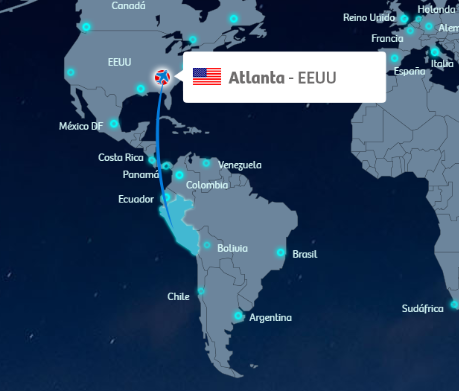
\includegraphics[keepaspectratio]{index_files/figure-html/lu137401d6rd_tmp_a545a4f3.png}}

}

\end{figure}%

\subsection{Análisis de la demanda}\label{anuxe1lisis-de-la-demanda}

El objetivo de esta sección es presentar la demanda de trucha para los 5
próximos años, usando métodos estadísticos. Eso nos permitirá determinar
cómo evolucionará el mercado de la trucha en Estados Unidos asimismo
planificar en el largo plazo las oportunidades para nuestra empresa.

\begin{enumerate}
\def\labelenumi{\alph{enumi})}
\tightlist
\item
  Demanda de productos sustitutos:
\end{enumerate}

El salmón que es directamente un sustituto de la trucha del otro lado,
tenemos los productos de comida marítima en lata que es una forma de
consumo muy importante en los hábitos de consumo de los estadounidenses.

\begin{itemize}
\tightlist
\item
  \hspace{0pt} \emph{El salmón:} La buena noticia es que el salmón ha
  ido escalando paulatinamente hasta sentarse en el segundo lugar de los
  productos del mar más importados por la nación norteamericana.
\end{itemize}

En los últimos años el consumo de salmón ha sido como la mostrada en la
tabla 3.11.

\begin{longtable}[]{@{}cc@{}}
\caption{Consumo per cápita de salmón 2009-2019 (En
libras)}\tabularnewline
\toprule\noalign{}
AÑO & CANTIDAD \\
\midrule\noalign{}
\endfirsthead
\toprule\noalign{}
AÑO & CANTIDAD \\
\midrule\noalign{}
\endhead
\bottomrule\noalign{}
\endlastfoot
2009 & 3.554 \\
2010 & 3.814 \\
2011 & 4.085 \\
2012 & 4.369 \\
2013 & 4.664 \\
2014 & 4.972 \\
2015 & 5.291 \\
2016 & 5.622 \\
2017 & 5.965 \\
2018 & 6.32 \\
2019 & 6.687 \\
\end{longtable}

\begin{itemize}
\item
  \hspace{0pt} \emph{Comida marítima en lata}: el atún y sus productos
  derivados se ubicaron en un tercer lugar, con US\$1.570 millones y
  385.825 toneladas; mientras que la tilapia se escaló hasta el cuarto
  puesto, al significar US\$673 millones y 172.546 toneladas.

  \begin{figure}[H]

  \caption{Productos sustitutos de la trucha en el mercado
  norteamericano}

  {\centering \pandocbounded{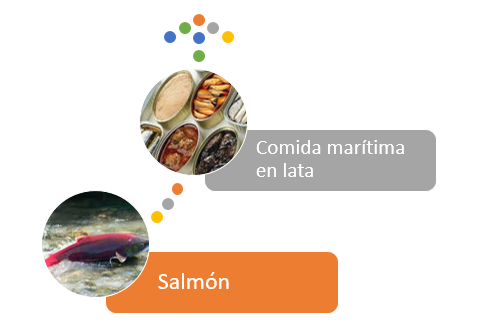
\includegraphics[keepaspectratio]{index_files/figure-html/lu137401d6rd_tmp_8ae05c66.png}}

  }

  \end{figure}%
\end{itemize}

\begin{enumerate}
\def\labelenumi{\alph{enumi})}
\setcounter{enumi}{1}
\tightlist
\item
  Selección del método de proyección:
\end{enumerate}

Los datos reales de importación obtenidos del Global Aquaculture
Alliance que se procesaran han sido ingresados al software estadístico
Minitab, a los cuales se les sometió a 6 de los modelos de proyección de
series de tiempo, resultando con menor error MAD el análisis de
tendencia cuadrática.

El objetivo de la identificación de la información histórica es
determinar un patrón básico en su comportamiento, que permita la
proyección futura de la variable deseada.

\begin{longtable}[]{@{}cc@{}}
\caption{Proyección de las importaciones de trucha a EE. UU (Solo filete
y trucha entera congelada)}\tabularnewline
\toprule\noalign{}
AÑO & PRONÓSTICO DE IMPORTACIONES EN Kg. \\
\midrule\noalign{}
\endfirsthead
\toprule\noalign{}
AÑO & PRONÓSTICO DE IMPORTACIONES EN Kg. \\
\midrule\noalign{}
\endhead
\bottomrule\noalign{}
\endlastfoot
2021 & 5465129 \\
2022 & 5637880 \\
2023 & 5810631 \\
2024 & 5983383 \\
2025 & 6156134 \\
\end{longtable}

\subsection{Tendencia general del
consumo}\label{tendencia-general-del-consumo}

\subsubsection{Segmentación
demográfica}\label{segmentaciuxf3n-demogruxe1fica}

Nuestro producto estará dirigido tanto a varones como mujeres que
pertenezcan a niveles socioeconómicos medio y alto, y cuyas edades
fluctúen entre los 25 y los 55 años.

\subsubsection{Segmentación
geográfica}\label{segmentaciuxf3n-geogruxe1fica}

Nuestro mercado principal es: Estados Unidos, Canadá y Japón. Partiendo
de ello, definimos que el foco inicial de nuestro mercado es EE. UU ya
que el primer país importador de pescados, que ocupa el cuarto lugar en
cuanto a población, con 328,2 millones (2019) habitantes que pertenecen
al nivel socioeconómico alto y medio.

\subsubsection{Segmentación
psicográfica}\label{segmentaciuxf3n-psicogruxe1fica}

Nuestro foco está compuesto por hombres y mujeres a quienes les interesa
mantener un estilo de vida saludable, que revisan el contenido
nutricional de los alimentos que consumen y el origen de estos.

\subsection{Análisis del comportamiento del
consumidor}\label{anuxe1lisis-del-comportamiento-del-consumidor}

\subsubsection{Hábitos de compra}\label{huxe1bitos-de-compra}

El consumidor estadounidense se muestra muy abierto a adquirir productos
extranjeros. El suministro de productos es muy diverso en Estados
Unidos. El consumidor estadounidense es rico y muy diverso en sus
intereses y sus gustos.

\subsubsection{Hábitos de consumo}\label{huxe1bitos-de-consumo}

Los estadounidenses se muestran cada vez más preocupados por los
ingredientes de su dieta: El 47\% evita los sabores artificiales y el
43\% los colorantes. Los ingredientes naturales son el tercer componente
más buscado en las etiquetas, después de aceites/grasas y edulcorantes.
La apuesta por lo natural también se refleja en la mayor demanda hacia
productos ricos en vitaminas en lugar de alimentos reforzados. Los
calificativos más buscados son `integral', `rico en fibra', `bajo en
sodio', `bajo en calorías', `sin grasas transgénicas', `bajo en azúcar',
`sin aditivos químicos' y `sin conservantes'.

\subsubsection{Medición de mercado}\label{mediciuxf3n-de-mercado}

\begin{longtable}[]{@{}lc@{}}
\caption{Consumo aparente}\tabularnewline
\toprule\noalign{}
Producción TM & 24233 \\
\midrule\noalign{}
\endfirsthead
\toprule\noalign{}
Producción TM & 24233 \\
\midrule\noalign{}
\endhead
\bottomrule\noalign{}
\endlastfoot
Importaciones (+) TM & 5016 \\
Exportaciones (-) TM & 1458 \\
Consumo Aparente (C.A) TM & 27791 \\
\end{longtable}

Esta tabla muestra el consumo aparente de trucha en el mercado
estadounidense, el cual se ha encontrado considerando la producción
nacional más las importaciones menos las exportaciones, quedando como
resultado un consumo aparente de \textbf{27,791 TM} al año.

\begin{longtable}[]{@{}lc@{}}
\caption{Consumo per - cápita}\tabularnewline
\toprule\noalign{}
Consumo Aparente (C.A) TM & 27791 \\
\midrule\noalign{}
\endfirsthead
\toprule\noalign{}
Consumo Aparente (C.A) TM & 27791 \\
\midrule\noalign{}
\endhead
\bottomrule\noalign{}
\endlastfoot
Población EE.UU. De 18 a más (2017) & 252063800 \\
Consumo per cápita TM & 0 \\
Consumo per cápita por Kg & 0.11 \\
\end{longtable}

\begin{longtable}[]{@{}lc@{}}
\caption{Razón de la cadena}\tabularnewline
\toprule\noalign{}
Método de la razón de la cadena & \\
\midrule\noalign{}
\endfirsthead
\toprule\noalign{}
Método de la razón de la cadena & \\
\midrule\noalign{}
\endhead
\bottomrule\noalign{}
\endlastfoot
Q (\$) = n\emph{p}q & \$30,470,049 \\
Q (Kg) = n*q & 2313595 \\
Q (TM) = Q(Kg)/1000 & 2313.6 \\
\% de mercado a conquistar & 0.45 \% \\
Demanda del mercado (Kg/año) & 10353 \\
(Kg/mes) & 863 \\
(TM/año) & 10.4 \\
(TM/mes) & 0.86 \\
Dda. Anual en Dólares & \$ 136,353 \\
Demanda Anual en Soles & S/. 449,966.45 \\
\end{longtable}

Donde:

Q = Demanda total del mercado

n = Población de Florida -EE.UU.

p = Precio del producto.

q = Consumo per-cápita kg.

n = 20,984,400

p = \$13.17

q = 0.1102531

La tabla muestra la demanda anual de trucha en el mercado
estadounidense, para el primer año la que asciende a 863 kg mensual,
considerando un porcentaje del 0.45\% del mercado a conquistar. Se
considera este porcentaje dado que es una estrategia de posicionamiento
en el mercado a conquistar, para entrar de manera sigilosa con respecto
a la competencia nacional para así no puedan generar barreras que
impidan la participación en el mercado internacional.

\subsection{Plan de marketing}\label{plan-de-marketing}

\subsubsection{Mix de marketing}\label{mix-de-marketing}

\begin{itemize}
\tightlist
\item
  \hspace{0pt} \textbf{Producto}
\end{itemize}

La trucha es un alimento de alto valor nutritivo para el ser humano en
todas sus etapas de desarrollo, especialmente durante la formación de un
nuevo ser y las primeras etapas de su crecimiento. Es una fuente rica en
componentes minerales como el calcio, fósforo, sodio y potasio. Contiene
omega 3 para el correcto funcionamiento de las actividades cerebrales,
capacidad del aprendizaje, reduce la viscosidad de la sangre, controla
los niveles de colesterol y de grasa, mejora la función del sistema
inmunológico.

\begin{itemize}
\tightlist
\item
  \hspace{0pt} \textbf{Precio}
\end{itemize}

El precio final de exportación de los filetes de trucha de 1000 gr. será
de US\$ 8.40. En este, se considera que el mercado de Estados Unidos
registra una alta preferencia por productos nutritivos y saludables.

Para poder llegar a este precio sugerido en el punto de venta, nuestra
empresa tendrá que negociar con el distribuidor las siguientes
condiciones:

Precio FCA Callao: US\$ 8.40 y forma de pago: carta de crédito
confirmada irrevocable

\begin{itemize}
\tightlist
\item
  \hspace{0pt} \textbf{Plaza}
\end{itemize}

El canal de distribución que se va a utilizar será indirecto, conformado
por el productor, exportador, supermercados y el consumidor final.

\begin{itemize}
\tightlist
\item
  \hspace{0pt} \textbf{Promoción}
\end{itemize}

Para dar a conocer nuestro producto se va a participar en ferias,
también se va a crear una página web, en la cual los consumidores podrán
verificar la información acerca de la procedencia del producto,
propiedades, beneficios, atributos, recetas, entre otros.

\subsubsection{Presupuesto de marketing}\label{presupuesto-de-marketing}

\begin{longtable}[]{@{}lc@{}}
\caption{Gasto en marketing con respecto a los ingresos por ventas
anuales}\tabularnewline
\toprule\noalign{}
GASTO EN PUBLICIDAD MENSUAL & 2183328 \\
\midrule\noalign{}
\endfirsthead
\toprule\noalign{}
GASTO EN PUBLICIDAD MENSUAL & 2183328 \\
\midrule\noalign{}
\endhead
\bottomrule\noalign{}
\endlastfoot
GASTO ANUAL & 26199936 \\
INGRESO POR VENTA ANUAL & 727776 \\
GASTO EN MARKETING SOBRE VENTAS & 0,3\% \\
\end{longtable}

En lo que respecta a Marketing se va a invertir el 0,3\% con respecto a
los ingresos netos por las ventas de filete refrigerado de trucha, el
que será utilizado para dar mantenimiento de la página web, así como
como para cubrir los gastos por viaje en ferias internacionales, en la
que se promocionará el producto.

\section{Capítulo IV Plan de
operación}\label{capuxedtulo-iv-plan-de-operaciuxf3n}

\subsection{Ficha de insumo producto}\label{ficha-de-insumo-producto}

\subsubsection{Insumos}\label{insumos}

\begin{table}

{\caption{{Ficha de insumo producto}{\label{tbl-mytable2}}}}

\begin{longtable}[]{@{}
  >{\raggedright\arraybackslash}p{(\linewidth - 2\tabcolsep) * \real{0.2917}}
  >{\raggedright\arraybackslash}p{(\linewidth - 2\tabcolsep) * \real{0.7083}}@{}}
\toprule\noalign{}
\begin{minipage}[b]{\linewidth}\raggedright
\textbf{Partida arancelaria:}
\end{minipage} & \begin{minipage}[b]{\linewidth}\raggedright
304420000
\end{minipage} \\
\midrule\noalign{}
\endhead
\bottomrule\noalign{}
\endlastfoot
\textbf{Nombre científico:} & Oncorhynchus mykiss \\
\textbf{Ventana comercial} & Venta de todo el año \\
\textbf{Descripción} & Filetes frescos o refrigerados de truchas. \\
\textbf{Presentación} & Filetes frescos o refrigerados de truchas
empacados al vacío en paquetes de 500g cada uno. \\
\textbf{Características fisicoquímicas:} & Composición por 100 gramos
por porción comestible - Calorías 89,8 - Grasas (g) 3.0 - Magnesio (mg)
28.0 - Fósforo (mg) 250 - Proteínas (g) 19,7 - Hiero (mg) 1,0 - Potasio
(mg) 250 - Zinc (mg) 0,8 \\
\textbf{Comentarios} & La trucha es muy consumida por el ser humano
debido a los grandes beneficios que nos puede aportar, entre los que
destacan: disminuye el sobrepeso, es buena para personas con
hipertensión arterial ya que tiene poca sal, y además es perfecta para
una dieta siempre y cuando esta sea combinada con un poco de ejercicios
diarios. \\
\end{longtable}

{\noindent \emph{Note.} Ministerio de comercio exterior y turismo}

\end{table}

\subsubsection{Gastos de fabricación}\label{gastos-de-fabricaciuxf3n}

\subsection{Cadena de producción}\label{cadena-de-producciuxf3n}

\begin{longtable}[]{@{}
  >{\raggedright\arraybackslash}p{(\linewidth - 6\tabcolsep) * \real{0.5500}}
  >{\centering\arraybackslash}p{(\linewidth - 6\tabcolsep) * \real{0.1500}}
  >{\raggedright\arraybackslash}p{(\linewidth - 6\tabcolsep) * \real{0.1500}}
  >{\raggedright\arraybackslash}p{(\linewidth - 6\tabcolsep) * \real{0.1500}}@{}}
\caption{Descripción de los procesos productivos para elaboración de
filete de trucha}\tabularnewline
\toprule\noalign{}
\begin{minipage}[b]{\linewidth}\raggedright
Descripción
\end{minipage} & \begin{minipage}[b]{\linewidth}\centering
Colaboradores
\end{minipage} & \begin{minipage}[b]{\linewidth}\raggedright
Tiempo
\end{minipage} & \begin{minipage}[b]{\linewidth}\raggedright
Recursos
\end{minipage} \\
\midrule\noalign{}
\endfirsthead
\toprule\noalign{}
\begin{minipage}[b]{\linewidth}\raggedright
Descripción
\end{minipage} & \begin{minipage}[b]{\linewidth}\centering
Colaboradores
\end{minipage} & \begin{minipage}[b]{\linewidth}\raggedright
Tiempo
\end{minipage} & \begin{minipage}[b]{\linewidth}\raggedright
Recursos
\end{minipage} \\
\midrule\noalign{}
\endhead
\bottomrule\noalign{}
\endlastfoot
1. Se compra la trucha a loa Distritos. & 1 & 1 hora & Centro de
Producción \\
2. Se recepciona el producto en planta de procesamiento, verificando su
tamaño y peso. & 2 & 1 hora & Canastas /Jabas, balanza \\
3. Se clasifica el producto por peso y tamaño & 1 & 2 horas & Canastas
/Jabas \\
4. El pescado es lavado con abundante agua potable libre de
contaminación y descamado con escobillas, eliminando posibles sangrados,
mucosidad y mejorando la apariencia del producto & 2 & 2 a 3 horas &
Descamador manual, tabla y agua \\
5. La trucha es eviscerada efectuando un corte ventral hasta la abertura
anal, con la finalidad de permitir el fácil acceso a la cavidad
abdominal para una completa eliminación del estómago y los restos de
vísceras. El descabezado se realiza con un corte perpendicular a la
espina dorsal, en forma recta, pasando por la zona donde roza el borde
más extremo del opérculo. & 2 & & Cuchillo y agua \\
6. se retiran todos los huesos pequeños que tiene la trucha & 2 & &
Cuchillo, agua y tabla \\
7. se procede a filetear el producto en pequeños cortes de 500 gr cada
uno & 2 & 1 hora & Cuchillos \\
8. La trucha eviscerada, descabezada y fileteada es lavada con abundante
agua potable, limpiando escrupulosamente la masa muscular eliminando
toda la sangre y posibles restos de intestinos u otros residuos. & 2 & 1
hora & Agua y tinas de metal \\
9. Se pesa el producto, se envasa en bolsas de polietileno y se sella
para ser refrigerado. & 1 & 1 horas & Bolsas de polietileno \\
10. Se refrigera el producto para luego ser empacado y almacenado. & 2 &
3 a 4 días & Cámara de congelación \\
11. Se empaca el producto & 2 & 5 horas & Cajas de cartón corrugado \\
12. Se almacena para luego ser exportado. & 2 & 1 hora & \\
\textbf{Total, de colaboradores.} & \textbf{6} & \textbf{3 a 4 días + 16
horas.} & \\
\end{longtable}

\textbf{Figura 4.1.}

\emph{Flujo del proceso productivo.}

\hspace{0pt}Adquisición de la trucha

\hspace{0pt}Recepción del producto

\hspace{0pt}\textbf{¿La trucha tiene el tamaño comercial?}

\hspace{0pt}Descarta

\hspace{0pt}Lavado y descamado

\hspace{0pt}Eviscerado y descabezado

\hspace{0pt}Deshuesado

\hspace{0pt}Pesado Envasado

\hspace{0pt}Lavado II

\hspace{0pt}Fileteado

\hspace{0pt}Sellado

\hspace{0pt}Refrigerado

\hspace{0pt}Empacado

\hspace{0pt}Almacenado

\subsection{Costos de producción}\label{costos-de-producciuxf3n}

Se ha considerado un incremento en la producción de 5\% anual, durante
los primeros cinco años, por lo tanto, se incrementan las materias
primas e insumos complementarios, siendo S/. 12.00 el costo unitario y
24.000 kg de trucha como la producción total en el primer año.

\subsubsection{Materia prima}\label{materia-prima}

\begin{longtable}[]{@{}
  >{\raggedright\arraybackslash}p{(\linewidth - 10\tabcolsep) * \real{0.3000}}
  >{\centering\arraybackslash}p{(\linewidth - 10\tabcolsep) * \real{0.1400}}
  >{\centering\arraybackslash}p{(\linewidth - 10\tabcolsep) * \real{0.1400}}
  >{\centering\arraybackslash}p{(\linewidth - 10\tabcolsep) * \real{0.1400}}
  >{\centering\arraybackslash}p{(\linewidth - 10\tabcolsep) * \real{0.1400}}
  >{\centering\arraybackslash}p{(\linewidth - 10\tabcolsep) * \real{0.1400}}@{}}
\caption{Cuadro de Costos de Producción}\tabularnewline
\toprule\noalign{}
\begin{minipage}[b]{\linewidth}\raggedright
\textbf{CONCEPTO}
\end{minipage} & \begin{minipage}[b]{\linewidth}\centering
\textbf{AÑOS}
\end{minipage} & \begin{minipage}[b]{\linewidth}\centering
\end{minipage} & \begin{minipage}[b]{\linewidth}\centering
\end{minipage} & \begin{minipage}[b]{\linewidth}\centering
\end{minipage} & \begin{minipage}[b]{\linewidth}\centering
\end{minipage} \\
\midrule\noalign{}
\endfirsthead
\toprule\noalign{}
\begin{minipage}[b]{\linewidth}\raggedright
\textbf{CONCEPTO}
\end{minipage} & \begin{minipage}[b]{\linewidth}\centering
\textbf{AÑOS}
\end{minipage} & \begin{minipage}[b]{\linewidth}\centering
\end{minipage} & \begin{minipage}[b]{\linewidth}\centering
\end{minipage} & \begin{minipage}[b]{\linewidth}\centering
\end{minipage} & \begin{minipage}[b]{\linewidth}\centering
\end{minipage} \\
\midrule\noalign{}
\endhead
\bottomrule\noalign{}
\endlastfoot
& \textbf{1} & \textbf{2} & \textbf{3} & \textbf{4} & \textbf{5} \\
\textbf{I. COSTOS DIRECTOS} & \textbf{339.050,00} & \textbf{357.327,50}
& \textbf{374.943,88} & \textbf{393.441,07} & \textbf{412.863,12} \\
Compra de trucha al por mayor & 300.000,00 & 315.000,00 & 330.750,00 &
347.287,50 & 364.651,88 \\
Compra de hielo en escamas & 1.050,00 & 1.102,50 & 1.157,63 & 1.215,51 &
1.276,28 \\
Bolsas para empaques con impresión & 2.000,00 & 2.100,00 & 2.205,00 &
2.315,25 & 2.431,01 \\
Mano de obra directa & 32.500,00 & 34.125,00 & 35.831,25 & 37.622,81 &
39.503,95 \\
Otros costos directos & 3.500,00 & 5.000,00 & 5.000,00 & 5.000,00 &
5.000,00 \\
\textbf{II. COSTOS INDIRECTOS} & \textbf{21.080,00} & \textbf{22.134,00}
& \textbf{23.240,70} & \textbf{24.402,74} & \textbf{25.622,87} \\
Mano de obra indirecta & 10.680,00 & 11.214,00 & 11.774,70 & 12.363,44 &
12.981,61 \\
Otros costos indirectos & 10.400,00 & 10.920,00 & 11.466,00 & 12.039,30
& 12.641,27 \\
\textbf{TOTAL COSTOS DE PRODUCCIÓN} & \textbf{360.130,00} &
\textbf{379.461,50} & \textbf{398.184,58} & \textbf{417.843,80} &
\textbf{438.485,99} \\
\end{longtable}

La tabla 4.3 muestra los costos de producción en los que la empresa
incurre. Se ha tenido en cuenta el incremento de 5\% de producción anual
para los años proyectados, donde se ha considerado como materia prima la
trucha viva que se va a comprar de los centros productivos de la región
a un precio de S/.10.00 el kg, comprando un promedio mensual de 2,500 kg
de trucha viva o 30,000 kg al año, lo que en promedio cuesta S/ 300,000;
también se ha considerado como materia prima el empaque a utilizar para
comercializar la trucha en el mercado estadounidense, en la que se
incluye. Cajas de Tecnoport, cajas de cartón (228 Uds. anual), etiquetas
especiales de exportación (18642 Uds. Anual), Gel pack (9,600 Uds.) y
bolsas de polietileno (18648 unidades, dado que por cada kg se necesita
2 bolsas) en a que se va envasar el filete de trucha refrigerado, el
monto de los costos totales para los años 1, 2, 3,4 y 5 están mostrados
en la tabla 4.3.

\subsubsection{Mano de obra}\label{mano-de-obra}

\begin{longtable}[]{@{}
  >{\raggedright\arraybackslash}p{(\linewidth - 8\tabcolsep) * \real{0.4600}}
  >{\centering\arraybackslash}p{(\linewidth - 8\tabcolsep) * \real{0.1200}}
  >{\centering\arraybackslash}p{(\linewidth - 8\tabcolsep) * \real{0.1200}}
  >{\centering\arraybackslash}p{(\linewidth - 8\tabcolsep) * \real{0.1500}}
  >{\centering\arraybackslash}p{(\linewidth - 8\tabcolsep) * \real{0.1500}}@{}}
\caption{Cuadro de Costos de la Mano de obra}\tabularnewline
\toprule\noalign{}
\begin{minipage}[b]{\linewidth}\raggedright
\textbf{Personal}
\end{minipage} & \begin{minipage}[b]{\linewidth}\centering
\textbf{Unidades}
\end{minipage} & \begin{minipage}[b]{\linewidth}\centering
\textbf{Cantidad (meses)}
\end{minipage} & \begin{minipage}[b]{\linewidth}\centering
\textbf{Costo Mensual (s/)}
\end{minipage} & \begin{minipage}[b]{\linewidth}\centering
\textbf{Costo Anual (S/)}
\end{minipage} \\
\midrule\noalign{}
\endfirsthead
\toprule\noalign{}
\begin{minipage}[b]{\linewidth}\raggedright
\textbf{Personal}
\end{minipage} & \begin{minipage}[b]{\linewidth}\centering
\textbf{Unidades}
\end{minipage} & \begin{minipage}[b]{\linewidth}\centering
\textbf{Cantidad (meses)}
\end{minipage} & \begin{minipage}[b]{\linewidth}\centering
\textbf{Costo Mensual (s/)}
\end{minipage} & \begin{minipage}[b]{\linewidth}\centering
\textbf{Costo Anual (S/)}
\end{minipage} \\
\midrule\noalign{}
\endhead
\bottomrule\noalign{}
\endlastfoot
\textbf{MANO DE OBRA DIRECTA} & & & & \textbf{144.000,00} \\
Personal planta de procesamiento (12 Personas) & Meses & 12 & 12.000,00
& 144.000,00 \\
\textbf{MANO DE OBRA INDIRECTA} & & & & \textbf{83.400,00} \\
Personal de control de calidad (1 Personal) & Meses & 12 & 1.200,00 &
14.400,00 \\
Jefe de producción & Meses & 12 & 2.000,00 & 24.000,00 \\
Técnico en producción & Meses & 12 & 1.500,00 & 18.000,00 \\
Almacenero & Meses & 12 & 750,00 & 9.000,00 \\
Vigilancia & Meses & 12 & 1.500,00 & 18.000,00 \\
\textbf{MANO DE OBRA ADMINISTRATIVA} & & & & \textbf{74.400,00} \\
Administrador & Meses & 12 & 2.000,00 & 24.000,00 \\
Secretaria & Meses & 12 & 800,00 & 9.600,00 \\
Contador & Meses & 12 & 1.000,00 & 12.000,00 \\
Chofer del proceso de producción & Meses & 12 & 1.200,00 & 14.400,00 \\
Chofer de la planta de procesamiento & Meses & 12 & 1.200,00 &
14.400,00 \\
\textbf{MANO DE OBRA DE VENTAS} & & & & \textbf{24.000,00} \\
Agente vendedor a todo costo & Meses & 12 & 2.000,00 & 24.000,00 \\
\textbf{COSTO TOTAL} & & & & \textbf{325.800,00} \\
\end{longtable}

Para la mano de obra directa se ha considerado el personal que tiene el
contacto directo con el producto, aquí se considera al personal que
recepciona, filetea, empaca y refrigera el producto, en esta etapa se
cuenta con 12 trabajadores los que tienen como remuneración S/ 38
diarios, llegando a requerir S/ 1000 mensual o S/ 14,400.00 anual, el
que se incrementa a lo largo de los años proyectados.

\subsubsection{Gastos de fabricación}\label{gastos-de-fabricaciuxf3n-1}

\begin{longtable}[]{@{}ll@{}}
\caption{Cuadro de gastos de fabricación.}\tabularnewline
\toprule\noalign{}
\textbf{CONCEPTO} & \textbf{COSTO TOTAL} \\
\midrule\noalign{}
\endfirsthead
\toprule\noalign{}
\textbf{CONCEPTO} & \textbf{COSTO TOTAL} \\
\midrule\noalign{}
\endhead
\bottomrule\noalign{}
\endlastfoot
\textbf{I. GASTOS ADMINISTRATIVOS} & \textbf{78.000,00} \\
Mano de obra administrativa & 74.400,00 \\
Útiles de oficina & 3.600,00 \\
\textbf{II. GASTOS GENERALES (5\% IF)} & \textbf{30.430,00} \\
\textbf{III. GASTOS DE SUPERVISIÓN (3\% IF)} & \textbf{18.258,00} \\
\textbf{TOTAL DE GASTOS DE FABRICACIÓN} & \textbf{126.688,00} \\
\end{longtable}

Los costos indirectos de fabricación (CIF) se ha considerado como gastos
generales conformado por los gastos por servicio de luz y agua, gastos
por supervisión y la depreciación de los activos fijos; también se ha
considerado la mano de obra indirecta conformada por el pago al personal
de mantenimiento y seguridad considerado en la tabla 4.5 denominada pago
de remuneraciones al personal administrativo.

\subsection{Estándares de calidad del producto o
servicio}\label{estuxe1ndares-de-calidad-del-producto-o-servicio}

El sistema de HACCP facilita la inspección por parte de las autoridades
encargadas de regular el control de los alimentos y favorece el comercio
internacional al aumentar la confianza de los compradores en la
inocuidad de los alimentos. Este sistema propone tener en cuenta lo
siguiente:

\textbf{1.} Independizar las distintas áreas de proceso del área de
producción propiamente dicha.

\textbf{2.} Priorizar, durante el proceso productivo, todas aquellas
medidas preventivas con el objeto de disminuir el riesgo de enfermedades
infecciosas y evitar de esta manera el uso de fármacos para combatirlas.

\textbf{3.} Extremar los cuidados de la higiene en las instalaciones del
emprendimiento. Ello implica no sólo el cuidado de la higiene del
personal sino también de los materiales que se utilizan en el proceso.

\section{Capítulo V Gestión
exportadora}\label{capuxedtulo-v-gestiuxf3n-exportadora}

\subsection{Análisis de costos y precios de
exportación}\label{anuxe1lisis-de-costos-y-precios-de-exportaciuxf3n}

\subsubsection{Elementos del precio de
exportación}\label{elementos-del-precio-de-exportaciuxf3n}

\begin{longtable}[]{@{}
  >{\raggedright\arraybackslash}p{(\linewidth - 2\tabcolsep) * \real{0.4167}}
  >{\raggedright\arraybackslash}p{(\linewidth - 2\tabcolsep) * \real{0.5833}}@{}}
\caption{Elementos e ítems del precio de exportación}\tabularnewline
\toprule\noalign{}
\begin{minipage}[b]{\linewidth}\raggedright
Elemento
\end{minipage} & \begin{minipage}[b]{\linewidth}\raggedright
Ítem
\end{minipage} \\
\midrule\noalign{}
\endfirsthead
\toprule\noalign{}
\begin{minipage}[b]{\linewidth}\raggedright
Elemento
\end{minipage} & \begin{minipage}[b]{\linewidth}\raggedright
Ítem
\end{minipage} \\
\midrule\noalign{}
\endhead
\bottomrule\noalign{}
\endlastfoot
Costo Del Producto & Fabricación \\
& Empaque especial para exportación \\
& Etiquetas especiales para exportación \\
& Embalaje \\
Costos De Transporte Y Seguro Interno & Fletes de fábrica a puerta
despacho \\
& Seguros de transporte (fábrica a puerto de despacho) \\
Costos Varios & Comisión para el agente de aduna, despachador \\
& Costo de documento(s) de exportación \\
& Costo de certificado de origen \\
Manejo De Carga & Utilización de instalaciones aeroportuarias \\
& Almacenaje \\
& Pesaje o cubicaje, carga \\
& Cargue y estiba \\
Costos Financieros & Crédito otorgado al comprador \\
& Póliza de seguro de crédito a la exportación \\
Otros Costos De Exportación & Varios (comisiones, envíos de muestras,
etc.) \\
& Costo FCA en aeropuerto de origen \\
\end{longtable}

\subsubsection{Costos y gastos de
exportación}\label{costos-y-gastos-de-exportaciuxf3n}

\begin{table}

{\caption{{Cálculo de costos estimados y precio FCA en
USD}{\label{tbl-mytable2}}}}

\begin{longtable}[]{@{}
  >{\raggedright\arraybackslash}p{(\linewidth - 4\tabcolsep) * \real{0.4930}}
  >{\raggedright\arraybackslash}p{(\linewidth - 4\tabcolsep) * \real{0.2535}}
  >{\raggedright\arraybackslash}p{(\linewidth - 4\tabcolsep) * \real{0.2535}}@{}}
\toprule\noalign{}
\begin{minipage}[b]{\linewidth}\raggedright
CÁLCULO DE COSTOS ESTIMADOS en USD y soles
\end{minipage} & \begin{minipage}[b]{\linewidth}\raggedright
\end{minipage} & \begin{minipage}[b]{\linewidth}\raggedright
\end{minipage} \\
\midrule\noalign{}
\endhead
\bottomrule\noalign{}
\endlastfoot
Costo total (Costo de fabricación-Producto terminado) & \$ 3,324. 09 &
S/.12002.89 \\
Costo de empaque (Envase, Empaque, Embalaje y Unitarización) & \$205.00
& S/.740.05 \\
Costo de Etiquetado, Marcado y Codificación & \$98.60 & S/.355.95 \\
Costo de Manipuleo en el local del exportador & \$144.00 & S/.519.84 \\
\textbf{Utilidad (25\%)} & \textbf{\$942.92} & \textbf{S/.3403.94} \\
\textbf{EX-WORK Total} & \textbf{\$4,714.61} & \textbf{17019.74} \\
Flete por transporte interno & \$609.42 & 250.61 \\
Estiba & \$15.85 & S/. 57.22 \\
Agente de Aduana & \$160.00 & S/.577.6 \\
Costos Operativos & \$ 277.01.00 & S/.1000 \\
FCA Total & \$5,766.89 & S/.20818.47 \\
\textbf{FCA Unitario} & \textbf{\$8.40} & \textbf{30.32} \\
\end{longtable}

{\noindent \emph{Note.} LATE-Simulador financiero (Promperú)}

\end{table}

Para el cálculo del precio FCA de exportación se tomó en cuenta un envió
de 1000 kilogramos, con medida de caja de 33 cm de alto, 80 cm de ancho,
60 cm de largo y con volumen de 26.40 cm3.

Para realizar el cálculo se consideran lo siguiente:

\begin{itemize}
\tightlist
\item
  \hspace{0pt} Tipo de cambio 3.61
\item
  \hspace{0pt} Contenedor de 20 pies
\item
  \hspace{0pt} Envío de 1000 Kg. De filete, 1kg por unidad.
\end{itemize}

Para obtener el costo total de fabricación se multiplicó el costo de
producción unitaria (S/.12.00) por la cantidad de envío. Además, se hizo
uso del simulador financiero LATE que Promperú nos brinda, el cual se
muestra en el Anexo No 1 y Anexo No 2.

\subsubsection{Selección del precio de
exportación}\label{selecciuxf3n-del-precio-de-exportaciuxf3n}

El precio que se seleccionó fue en función al mercado, es decir, en base
a los precios fijados por la competencia.

Para ello se tomó como referencia el promedio del precio FOB de
exportación de los dos últimos dos años de exportación, estos se
muestran en la Tabla 5.3.

\begin{table}

{\caption{{Precio FOB promedio de las exportaciones de PERÚ en los
últimos 2 años hacia EE. UU}{\label{tbl-mytable2}}}}

\begin{longtable}[]{@{}lclc@{}}
\toprule\noalign{}
\textbf{2018} & & \textbf{2019} & \\
\midrule\noalign{}
\endhead
\bottomrule\noalign{}
\endlastfoot
ENERO & 11.73 & ENERO & 6.26 \\
FEBRERO & 11.79 & FEBRERO & 6.29 \\
MARZO & 11.76 & MARZO & 6.41 \\
ABRIL & 11.74 & ABRIL & 6.92 \\
MAYO & 11.68 & MAYO & 7.36 \\
JUNIO & 11.68 & JUNIO & 7.93 \\
JULIO & 11.73 & JULIO & 6.33 \\
AGOSTO & 11.28 & AGOSTO & 6.33 \\
SETIEMBRE & 6.52 & SETIEMBRE & 7.25 \\
OCTUBRE & 6.43 & OCTUBRE & 7.19 \\
NOVIEMBRE & 6.44 & NOVIEMBRE & 7.15 \\
DICIEMBRE & 6.19 & DICIEMBRE & 7.15 \\
\textbf{TOTAL PROMEDIO} & \textbf{8.398} & & \\
\end{longtable}

{\noindent \emph{Note.} SIICEX SUNAT}

\end{table}

\subsection{Modalidades de pago}\label{modalidades-de-pago}

\subsubsection{Forma de pago}\label{forma-de-pago}

La forma de pago que se utilizará en la transacción será el \textbf{pago
a plazo,} la empresa ofrecerá una facilidad de pago y crédito al
comprador. Esto debido a que existe confianza entre el comprador y el
vendedor y a que también el comprador goza de un buen nivel de crédito.

\subsubsection{Entrega de mercancía}\label{entrega-de-mercancuxeda}

Para la entrega de la mercancía se consideró el Incoterm FCA. A
continuación, estableceremos el punto de entrega:

La mercancía será entregada en las bodegas del avión, por tanto, toda la
operatividad, incluso la disposición de la mercancía ante aduana y el
despacho de exportación será responsabilidad de la empresa exportadora
Aquazul.

\subsubsection{Cobro}\label{cobro}

El cobro se realizará mediante un pago de transferencia de cuenta a
cuenta, en donde tanto el exportador como el importador deben contar
obligatoriamente con una cuenta bancaria para que el comprador ordene la
transferencia de dinero del banco de origen al banco de destino. Este
cobro podrá realizarse mediante el Banco de Crédito del Perú.

\subsection{Riesgos}\label{riesgos}

Al momento de realizar la venta al mercado internacional se considerara
diversos riesgos y para enfrentarse de una manera adecuada se tomara las
previsiones respectivas, como tener un seguro de carga internacional el
cual permite asegurar la mercancía en caso de ocurrir un posible
siniestro, también existe el riesgo de que el importador o comprador
reciba la mercadería y se niegue a pagarla , para evitar este tipo de
incidente la empresa Aquazul realizara el tipo de cobranza internacional
a través de la carta de crédito a través del Banco de Crédito del Perú.

\subsection{Cartas de crédito}\label{cartas-de-cruxe9dito}

\begin{figure}[H]

\caption{Costos de Carta de Crédito de Exportación de los distintos
entes bancarios peruanos.}

{\centering \pandocbounded{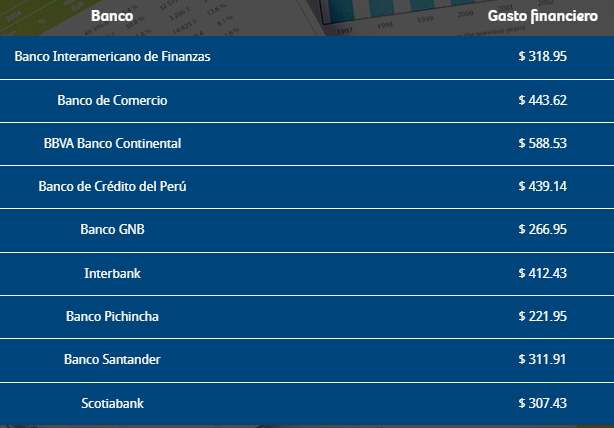
\includegraphics[keepaspectratio]{index_files/figure-html/lu137401d6rd_tmp_7f771699.png}}

}

\end{figure}%

En el cuadro se muestra los distintos costos de una carta de crédito
que, en la exportación, este se calculó con un envió de 1000 unidades de
filete de trucha de 1kg. Con un monto total de cobro de \$42,381.40 en
30 días. Se opto por el Banco de Crédito del Perú, debido a su
eficiencia y seguridad. 2,381.40 - 30

\subsection{Distribución física
internacional}\label{distribuciuxf3n-fuxedsica-internacional}

\textbf{Logística internacional -- DFI}

\subsubsection{Proceso de
Unitarización}\label{proceso-de-unitarizaciuxf3n}

\textbf{a. Envase Primario}

Descripción del envase: bolsa de polietileno

Cantidad de productos: 1000 g en una bolsa

\begin{longtable}[]{@{}ccc@{}}
\toprule\noalign{}
LARGO CM & ANCHO CM & ALTO CM \\
\midrule\noalign{}
\endhead
\bottomrule\noalign{}
\endlastfoot
30 & 20 & 5 \\
\end{longtable}

\textbf{b. Envase secundario}

Descripción del envase: Caja de tecnoport.

Cantidad de productos: 40 kg en una caja.

\begin{longtable}[]{@{}ccc@{}}
\toprule\noalign{}
LARGO CM & ANCHO CM & ALTO CM \\
\midrule\noalign{}
\endhead
\bottomrule\noalign{}
\endlastfoot
60 & 80 & 33 \\
\end{longtable}

\textbf{c.~Paletización}

Descripción del envase: Paletas de madera

Cantidad de productos: 200 Kg de filete de trucha congelada en cada
pallet

\begin{longtable}[]{@{}ccc@{}}
\toprule\noalign{}
LARGO CM & ANCHO CM & ALTO CM \\
\midrule\noalign{}
\endhead
\bottomrule\noalign{}
\endlastfoot
120 & 80 & 0.15 \\
\end{longtable}

\textbf{d.~Contenedor}

Descripción del envase: Contenedor RMP con temperatura regulable con
código por la Asociación Internacional de Transporte Aéreo (IATA), por
sus siglas en inglés. Contenedor con espuma de poliéster entre los
paneles laterales. Temperatura controlada entre 0 + 20° C. Apertura con
puerta sellable. Comportamiento con capacidad de hasta 400 kg de hielo
seco con espacio para baterías de ventilador en un lado.

\subsubsection{Utilización de embalajes: Rotulados e
Etiquetado}\label{utilizaciuxf3n-de-embalajes-rotulados-e-etiquetado}

\begin{enumerate}
\def\labelenumi{\alph{enumi})}
\tightlist
\item
  Envase Primario
\end{enumerate}

Rotulado: Señalización y Código de barras

Etiquetado: País de origen, marcas de peso, número de paquete y
dimensiones de la caja, puerto de entrada, marcas del consignatario,
marcas de advertencia, marca de manipuleo, marca del embarcador, los
datos en español e inglés.

\begin{enumerate}
\def\labelenumi{\alph{enumi})}
\setcounter{enumi}{1}
\tightlist
\item
  Palatización
\end{enumerate}

Rotulado: Reglamentos técnicos específicos sobre etiquetados de
determinados productos para EE.UU (variedad del producto, material del
empaque, tamaño, cantidades por empaque en español e inglés)

\begin{enumerate}
\def\labelenumi{\alph{enumi})}
\setcounter{enumi}{2}
\tightlist
\item
  Contenedor
\end{enumerate}

Rotulado: Reglamentos técnicos específicos sobre etiquetados de
determinados productos para EE.UU. (packinglist, número de contenedor,
temperatura registrada del contenedor, número de pallets, nombre de la
empresa comercializadora, aeropuerto de origen, aeropuerto de destino).

\subsection{Análisis de riesgo de
operarios}\label{anuxe1lisis-de-riesgo-de-operarios}

El país comprador de nuestro producto será Estados Unidos, por ello se
realizará un análisis de sus indicadores macroeconómicos.

Estados Unidos es la mayor economía a nivel mundial, por sobre China. La
economía creció 2,3\% en 2019 ---en comparación con 2,9\% en 2018--- y
se estima que el crecimiento caerá a -5,9\% en 2020 debido al brote de
COVID-19, y que luego repuntará a 4,7\% en 2021, según las últimas
estimaciones del FMI (del 14 de abril de 2020). La guerra comercial
entre Estados Unidos y China parece afectar a los inversores y a la
economía en su conjunto. El presidente Trump implementó medidas de
proteccionismo comercial a través de aranceles aplicados a las
importaciones chinas, y a pesar de que se anunció un acuerdo comercial
parcial en diciembre de 2019, según Coface se prevé que las tensiones se
prolonguen y que se mantengan los aranceles (19\% en promedio en enero
de 2020, en comparación con 3\% a principios de 2018).

El FMI prevé que la deuda pública crezca a 106,2\% en 2019. Esta
tendencia debiera continuar en 2020 y 2021. El déficit fiscal de Estados
Unidos llegó a -6,3\% en 2019, y debiera estabilizarse en los próximos
años. Las reformas fiscales del presidente Trump han afectado el déficit
desde 2018, generando una tendencia al alza para la deuda. Los
economistas estiman que el gobierno seguirá aumentando el gasto. Según
el FMI, la tasa de inflación bajó a 1,8\% en 2019, cerca del objetivo de
2\% fijado por la Reserva Federal. La tasa de inflación debiera subir
nuevamente en 2020 y 2021 por sobre 2\%.

La tasa de desempleo bajó de 3,9\% a 3.7\% en 2019. Sin embargo, el FMI
prevé que esta tendencia se vea fuertemente afectada por el impacto
económico negativo de la pandemia de COVID-19: estima actualmente que la
tasa aumentará a 10,4\% en 2020 y bajará ligeramente a 9,1\% en 2021.

\begin{figure}[H]

\caption{Principales Indicadores Macroeconómicos.}

{\centering \pandocbounded{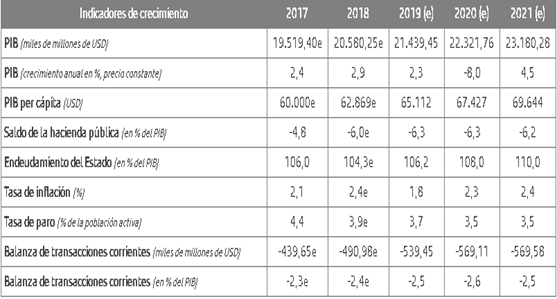
\includegraphics[keepaspectratio]{index_files/figure-html/lu137401d6rd_tmp_75d8738e.png}}

}

\end{figure}%%
\begin{figure}[H]

\caption{Perspectivas económicas mundiales-Pronósticos.}

{\centering \pandocbounded{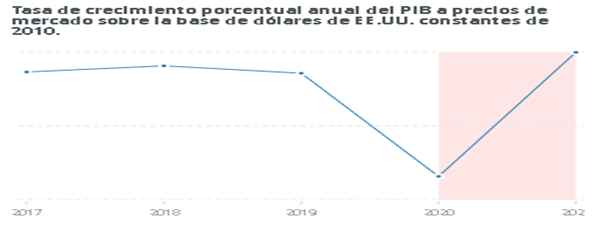
\includegraphics[keepaspectratio]{index_files/figure-html/lu137401d6rd_tmp_f1548be1.png}}

}

\end{figure}%

\textbf{Operador Logístico}

El operador logístico con quien se va trabajar es la empresa ``New
Atlantic S.A.C'' cuya información se detalla en la siguiente tabla.

\begin{longtable}[]{@{}
  >{\raggedright\arraybackslash}p{(\linewidth - 2\tabcolsep) * \real{0.4000}}
  >{\raggedright\arraybackslash}p{(\linewidth - 2\tabcolsep) * \real{0.6000}}@{}}
\caption{Ficha empresarial del operador logístico}\tabularnewline
\toprule\noalign{}
\begin{minipage}[b]{\linewidth}\raggedright
Nombre comercial
\end{minipage} & \begin{minipage}[b]{\linewidth}\raggedright
Natsac
\end{minipage} \\
\midrule\noalign{}
\endfirsthead
\toprule\noalign{}
\begin{minipage}[b]{\linewidth}\raggedright
Nombre comercial
\end{minipage} & \begin{minipage}[b]{\linewidth}\raggedright
Natsac
\end{minipage} \\
\midrule\noalign{}
\endhead
\bottomrule\noalign{}
\endlastfoot
RUC & 20562763351 \\
Razón social & New atlantic sac \\
Tipo de dirección & Oficina Comercia \\
Dirección & Av Oscar Benavides 4595-201 callao \\
País & Perú \\
Departamento & LIMA \\
Provincia & CALLAO \\
Distrito & CALLAO \\
Teléfono Oficina & 14697815 \\
Teléfono Celular & 981366393 \\
Correo &
\href{mailto:luis.mogrovejo@new-atlantic.com}{\nolinkurl{luis.mogrovejo@new-atlantic.com}} \\
Página Web & https://www.new-atlantic.com/nosotros.php \\
Persona de Contacto & Luis angel mogrovejo ramos \\
Descripción de la empresa & New atlantic sac, brinda servicio logistico
door to door, ofrecemos la venta de fletes, seguros, servicio de
agenciamiento, transporte local. \\
\end{longtable}

\subsection{Manejo documentario}\label{manejo-documentario}

\subsubsection{Documentos comerciales}\label{documentos-comerciales}

\paragraph{Factura comercial.}\label{factura-comercial}

\begin{figure}[H]

\caption{Factura comercial}

{\centering \pandocbounded{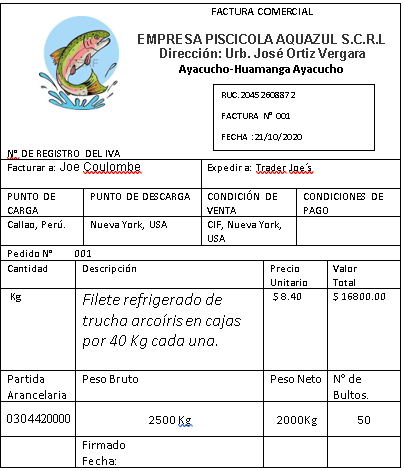
\includegraphics[keepaspectratio]{index_files/figure-html/lu137401d6rd_tmp_822257a8.png}}

}

\end{figure}%

\subsubsection{Certificados exigidos}\label{certificados-exigidos}

\paragraph{Certificado de origen.}\label{certificado-de-origen.}

Nuestro producto tendrá como destino el mercado estadounidense por el
cual según el Ministerio de Comercio Exterior y Turismo se tiene que
hacer una Auto-certificación en el cual el exportador puede emitir de
manera directa un certificado de origen en caso desee que su mercancía
ingrese a los mercados de Estados Unidos, Canadá y Corea del Sur (esta
modalidad es aplicable solo para estos países).

\subsection{Modelo de cotización}\label{modelo-de-cotizaciuxf3n}

\begin{longtable}[]{@{}
  >{\raggedright\arraybackslash}p{(\linewidth - 6\tabcolsep) * \real{0.3000}}
  >{\raggedright\arraybackslash}p{(\linewidth - 6\tabcolsep) * \real{0.3400}}
  >{\raggedright\arraybackslash}p{(\linewidth - 6\tabcolsep) * \real{0.1800}}
  >{\raggedright\arraybackslash}p{(\linewidth - 6\tabcolsep) * \real{0.1800}}@{}}
\toprule\noalign{}
\begin{minipage}[b]{\linewidth}\raggedright
\textbf{Aquazul S.C.R. L}
\end{minipage} & \begin{minipage}[b]{\linewidth}\raggedright
COTIZACIÓN N°001-2020
\end{minipage} & \begin{minipage}[b]{\linewidth}\raggedright
\end{minipage} & \begin{minipage}[b]{\linewidth}\raggedright
\end{minipage} \\
\midrule\noalign{}
\endhead
\bottomrule\noalign{}
\endlastfoot
Fecha De Cotización & 21/09/20 & Empresa De Destino & Trader Joe´s \\
Nombre De Destinatario & Joe Coulombe & & \\
Dirección De La Empresa &
\href{https://www.tripadvisor.com.pe/Restaurant_Review-g60763-d1099366-Reviews-Trader_Joe-New_York_City_New_York.html\#MAPVIEW}{142
E 14th St, Nueva York, NY 10003-4170} & & \\
País Destino & EE.UU & Referencia & Nueva York \\
Partida Arancelaria & 304420000 & Producto & Filete refrigerado de
trucha Arcoíris \\
Descripción De La Calidad & Producto natural y saludable & Cantidad &
2000Kg \\
Precio Fca Unitario & \$ 8.40 & Precio Fca Total & \$ 16800.00 \\
Moneda De Cotización & Dólar americano & & \\
Forma De Pago & El 50\% 15 días antes de la entrega de la mercancía y el
50\% restante cuando la mercancía llega al aeropuerto de destino & & \\
Fecha De Embarque & 30/05/21 & Medio De Transporte & Aéreo \\
Aeropuerto De Embarque & Puerto internacional Callao-LimaPerú. &
Aeropuerto De Llegada & Nueva York \\
\end{longtable}

\section{Capítulo VI Análisis financiero y plan
financiero}\label{capuxedtulo-vi-anuxe1lisis-financiero-y-plan-financiero}

\subsection{Análisis financiero}\label{anuxe1lisis-financiero}

\subsubsection{Análisis del balance general y estructura del balance
general}\label{anuxe1lisis-del-balance-general-y-estructura-del-balance-general}

\begin{longtable}[]{@{}
  >{\raggedright\arraybackslash}p{(\linewidth - 10\tabcolsep) * \real{0.5000}}
  >{\centering\arraybackslash}p{(\linewidth - 10\tabcolsep) * \real{0.1000}}
  >{\centering\arraybackslash}p{(\linewidth - 10\tabcolsep) * \real{0.1000}}
  >{\centering\arraybackslash}p{(\linewidth - 10\tabcolsep) * \real{0.1000}}
  >{\centering\arraybackslash}p{(\linewidth - 10\tabcolsep) * \real{0.1000}}
  >{\centering\arraybackslash}p{(\linewidth - 10\tabcolsep) * \real{0.1000}}@{}}
\caption{Balance general al 31 de diciembre con financiamiento,
proyectado}\tabularnewline
\toprule\noalign{}
\endfirsthead
\endhead
\bottomrule\noalign{}
\endlastfoot
& \textbf{1} & \textbf{2} & \textbf{3} & \textbf{4} & \textbf{5} \\
\textbf{Activo} & & & & & \\
\textbf{Activo corriente} & & & & & \\
Efectivo y equivalente de efectivo & 39050 & 75400 & 117200 & 157101 &
202990 \\
Cuentas por cobrar comerciales & & 28750 & 29880 & 30500 & 30550 \\
\textbf{Total activo corriente} & \textbf{39050} & \textbf{104150} &
\textbf{147080} & \textbf{187601} & \textbf{233540} \\
Activo no corriente & & & & & \\
IME(Neto) & 132115 & 123134 & 112142 & 101136 & 90140 \\
Intangibles & 2156 & 1702 & 1080 & 652 & \\
\textbf{Total activo no corriente} & \textbf{134271} & \textbf{124836} &
\textbf{113222} & \textbf{101788} & \textbf{90140} \\
\textbf{Total activo} & \textbf{173321} & \textbf{228986} &
\textbf{260302} & \textbf{289389} & \textbf{323680} \\
\textbf{Pasivo} & & & & & \\
Pasivo corriente & & & & & \\
Obligaciones financieras C-P & 16200 & 18202 & 25115 & 31269 & 0 \\
Gastos por tributos & & 16400 & 17950 & 22845 & 25987 \\
\textbf{Total pasivo corriente} & \textbf{16200} & \textbf{34602} &
\textbf{43065} & \textbf{54114} & \textbf{25987} \\
Pasivo no corriente & & & & & \\
Obligaciones financieras L-P & 72850 & 55645 & 29894 & 0 & 0 \\
\textbf{Total pasivo no corriente} & \textbf{72850} & \textbf{55645} &
\textbf{29894} & \textbf{0} & \textbf{0} \\
\textbf{Total pasivo} & \textbf{89050} & \textbf{90247} & \textbf{72959}
& \textbf{54114} & \textbf{25987} \\
\textbf{Patrimonio} & & & & & \\
Capital & 68450 & 102450 & 102450 & 102450 & 102450 \\
Resultados acumulados & & 39854 & 85231 & 138102 & 196689 \\
\textbf{Total patrimonio} & \textbf{68450} & \textbf{142304} &
\textbf{187681} & \textbf{240552} & \textbf{299139} \\
\textbf{Total pasivo y patrimonio} & \textbf{157500} & \textbf{232551} &
\textbf{260640} & \textbf{294666} & \textbf{325126} \\
\end{longtable}

En la tabla 6.1. se muestra el balance general con financiamiento desde
el año 1 hasta el año 5 del proyecto, todos ellos muestran resultados al
31 de diciembre para cada año, excepto en el año 1 en el que se realizan
todas las inversiones iniciales para que el proyecto se lleve a cabo, en
este año se considera dentro del activo corriente al efectivo y
equivalente de efectivo, y es el resultante de la diferencia del ingreso
mensual y el egreso mensual que es de S/ 39,050; que es el monto
necesario para que empiece a funcionar el proyecto; la utilidad antes
del impuesto a la renta, depreciación de maquinaria, construcciones,
amortización de intangibles todo ello menos amortización de la deuda y
cuentas por cobrar comerciales dando una cantidad de S/ 75,400; y así
sucesivamente se repite el proceso hasta llegar al año 5.

En el patrimonio se considera el capital aportado por los
inversionistas, que para el año 1 y 2 es de S/ 68,450; para el año 2
este incrementa dado que se le suma la utilidad del año 1.

\subsubsection{Análisis horizontal}\label{anuxe1lisis-horizontal}

\begin{longtable}[]{@{}
  >{\raggedright\arraybackslash}p{(\linewidth - 20\tabcolsep) * \real{0.2000}}
  >{\centering\arraybackslash}p{(\linewidth - 20\tabcolsep) * \real{0.0800}}
  >{\centering\arraybackslash}p{(\linewidth - 20\tabcolsep) * \real{0.0800}}
  >{\centering\arraybackslash}p{(\linewidth - 20\tabcolsep) * \real{0.0800}}
  >{\centering\arraybackslash}p{(\linewidth - 20\tabcolsep) * \real{0.0800}}
  >{\centering\arraybackslash}p{(\linewidth - 20\tabcolsep) * \real{0.0800}}
  >{\centering\arraybackslash}p{(\linewidth - 20\tabcolsep) * \real{0.0800}}
  >{\centering\arraybackslash}p{(\linewidth - 20\tabcolsep) * \real{0.0800}}
  >{\centering\arraybackslash}p{(\linewidth - 20\tabcolsep) * \real{0.0800}}
  >{\centering\arraybackslash}p{(\linewidth - 20\tabcolsep) * \real{0.0800}}
  >{\centering\arraybackslash}p{(\linewidth - 20\tabcolsep) * \real{0.0800}}@{}}
\caption{Balance general al 31 de diciembre con financiamiento,
proyectado}\tabularnewline
\toprule\noalign{}
\endfirsthead
\endhead
\bottomrule\noalign{}
\endlastfoot
\textbf{AÑOS} & \textbf{1 a 2} & \textbf{2 a 3} & \textbf{3 a 4} &
\textbf{4 a 5} & \textbf{1 a 5} & \textbf{1 a 2} & \textbf{2 a 3} &
\textbf{3 a 4} & \textbf{4 a 5} & \textbf{1 a 5} \\
\textbf{Activo} & & & & & & & & & & \\
\textbf{Activo corriente} & & & & & & & & & & \\
Efectivo y equivalente de efectivo & 36350 & 41800 & 39901 & 45889 &
163940 & 93 \% & 55 \% & 34 \% & 29 \% & 420 \% \\
Cuentas por cobrar comerciales & 28750 & 1130 & 620 & 50 & 30550 & & 4
\% & 2 \% & 0 \% & \\
\textbf{Total activo corriente} & \textbf{65100} & \textbf{42930} &
\textbf{40521} & \textbf{45939} & \textbf{194490} & \textbf{167 \%} &
\textbf{41 \%} & \textbf{28 \%} & \textbf{24 \%} & \textbf{498 \%} \\
\textbf{Activo no corriente} & & & & & & & & & & \\
IME(Neto) & -8981 & -10992 & -11006 & -10996 & -41975 & -7 \% & -9 \% &
-10 \% & -1 \% & -32 \% \\
Intangibles & -454 & -622 & -428 & -652 & -2156 & -21 \% & -37 \% & -40
\% & -100 \% & -100 \% \\
\textbf{Total activo no corriente} & \textbf{-9435} & \textbf{-11614} &
\textbf{-11434} & \textbf{-11648} & \textbf{-44131} & \textbf{-7 \%} &
\textbf{-9 \%} & \textbf{-10 \%} & \textbf{-11 \%} & \textbf{-33 \%} \\
\textbf{Total activo} & \textbf{55665} & \textbf{31316} & \textbf{29087}
& \textbf{34291} & \textbf{150359} & \textbf{32 \%} & \textbf{14 \%} &
\textbf{11 \%} & \textbf{12 \%} & \textbf{87 \%} \\
\textbf{Pasivo} & & & & & & & & & & \\
\textbf{Pasivo corriente} & & & & & & & & & & \\
Obligaciones financieras C-P & 2002 & 6913 & 6154 & -31269 & -16200 & 12
\% & 38 \% & 25 \% & -100 \% & -100 \% \\
Gastos por tributos & 16400 & 1550 & 4895 & 3142 & 25987 & & 9 \% & 27
\% & 14 \% & \\
\textbf{Total pasivo corriente} & \textbf{18402} & \textbf{8463} &
\textbf{11049} & \textbf{-28127} & \textbf{9787} & \textbf{114 \%} &
\textbf{24 \%} & \textbf{26 \%} & \textbf{-52 \%} & \textbf{60 \%} \\
\textbf{Pasivo no corriente} & & & & & & & & & & \\
Obligaciones financieras L-P & -17205 & -25751 & -29894 & 0 & -72850 &
-24 \% & -46 \% & -100 \% & & -100 \% \\
\textbf{Total pasivo no corriente} & \textbf{-17205} & \textbf{-25751} &
\textbf{-29894} & \textbf{0} & \textbf{-72850} & \textbf{-24 \%} &
\textbf{-46 \%} & \textbf{-100 \%} & & \textbf{-100 \%} \\
\textbf{Total pasivo} & \textbf{1197} & \textbf{-17288} &
\textbf{-18845} & \textbf{-28127} & \textbf{-63063} & \textbf{1 \%} &
\textbf{-19 \%} & \textbf{-26 \%} & \textbf{-52 \%} & \textbf{-71 \%} \\
\textbf{Patrimonio} & & & & & & & & & & \\
Capital & 34000 & 0 & 0 & 0 & 34000 & 50 \% & 0 \% & 0 \% & 0 \% & 50
\% \\
Resultados acumulados & 39854 & 45377 & 52871 & 58587 & 196689 & & 114
\% & 62 \% & 42 \% & \\
\textbf{Total patrimonio} & \textbf{73854} & \textbf{45377} &
\textbf{52871} & \textbf{58587} & \textbf{230689} & \textbf{108 \%} &
\textbf{32 \%} & \textbf{28 \%} & \textbf{24 \%} & \textbf{337 \%} \\
\textbf{Total pasivo y patrimonio} & \textbf{75051} & \textbf{28089} &
\textbf{34026} & \textbf{30460} & \textbf{167626} & \textbf{48 \%} &
\textbf{12 \%} & \textbf{13 \%} & \textbf{10 \%} & \textbf{106 \%} \\
\end{longtable}

En la tabla 6.2. se muestra el análisis horizontal del balance general
con financiamiento desde el año 1 hasta el año 5 del proyecto, todos
ellos muestran resultados al 31 de diciembre para cada año, en el año 1
se considera dentro del activo corriente al efectivo y equivalente de
efectivo los cuales presentan crecimientos de 93\% en el primer año y de
un 420\% en los 5 años; con respecto a las cuentas por cobrar
comerciales en el año 1 no se presenta un aumento porcentual, ya para el
año 2 el porcentaje es de 41\%. Para el activo no corriente se ha
considerado el costo total de los inmuebles, maquinaria y equipo se tuvo
una reducción de 7\%; para los años siguientes desde el año 1 hasta el
año 5 se tuvo una disminución en 32\%.

Ya que en el pasivo corriente está formado por las obligaciones
financieras a corto plazo el cual en el año 1 al año 5 asciende a S/ 0
no presenta ningún crecimiento, dado que en el balance general mostrado
no se considera préstamo; aquí se considera los gastos por tributos
formado por el impuesto tuvo un crecimiento de 1\% en el primer año y
una disminución de 71\% en los 5 años. En el patrimonio se considera el
capital aportado por los inversionistas, que para los años del 1 al 5
presenta un incremento de 50\%.

\subsubsection{Análisis vertical}\label{anuxe1lisis-vertical}

\begin{longtable}[]{@{}
  >{\raggedright\arraybackslash}p{(\linewidth - 22\tabcolsep) * \real{0.1300}}
  >{\centering\arraybackslash}p{(\linewidth - 22\tabcolsep) * \real{0.0700}}
  >{\centering\arraybackslash}p{(\linewidth - 22\tabcolsep) * \real{0.0700}}
  >{\centering\arraybackslash}p{(\linewidth - 22\tabcolsep) * \real{0.0700}}
  >{\centering\arraybackslash}p{(\linewidth - 22\tabcolsep) * \real{0.0700}}
  >{\centering\arraybackslash}p{(\linewidth - 22\tabcolsep) * \real{0.0700}}
  >{\raggedright\arraybackslash}p{(\linewidth - 22\tabcolsep) * \real{0.1300}}
  >{\centering\arraybackslash}p{(\linewidth - 22\tabcolsep) * \real{0.0700}}
  >{\centering\arraybackslash}p{(\linewidth - 22\tabcolsep) * \real{0.0700}}
  >{\centering\arraybackslash}p{(\linewidth - 22\tabcolsep) * \real{0.0700}}
  >{\centering\arraybackslash}p{(\linewidth - 22\tabcolsep) * \real{0.0700}}
  >{\centering\arraybackslash}p{(\linewidth - 22\tabcolsep) * \real{0.0700}}@{}}
\caption{Balance general al 31 de diciembre con financiamiento,
proyectado}\tabularnewline
\toprule\noalign{}
\begin{minipage}[b]{\linewidth}\raggedright
\end{minipage} & \begin{minipage}[b]{\linewidth}\centering
\textbf{AÑO}
\end{minipage} & \begin{minipage}[b]{\linewidth}\centering
\end{minipage} & \begin{minipage}[b]{\linewidth}\centering
\end{minipage} & \begin{minipage}[b]{\linewidth}\centering
\end{minipage} & \begin{minipage}[b]{\linewidth}\centering
\end{minipage} & \begin{minipage}[b]{\linewidth}\raggedright
\end{minipage} & \begin{minipage}[b]{\linewidth}\centering
\textbf{AÑO}
\end{minipage} & \begin{minipage}[b]{\linewidth}\centering
\end{minipage} & \begin{minipage}[b]{\linewidth}\centering
\end{minipage} & \begin{minipage}[b]{\linewidth}\centering
\end{minipage} & \begin{minipage}[b]{\linewidth}\centering
\end{minipage} \\
\midrule\noalign{}
\endfirsthead
\toprule\noalign{}
\begin{minipage}[b]{\linewidth}\raggedright
\end{minipage} & \begin{minipage}[b]{\linewidth}\centering
\textbf{AÑO}
\end{minipage} & \begin{minipage}[b]{\linewidth}\centering
\end{minipage} & \begin{minipage}[b]{\linewidth}\centering
\end{minipage} & \begin{minipage}[b]{\linewidth}\centering
\end{minipage} & \begin{minipage}[b]{\linewidth}\centering
\end{minipage} & \begin{minipage}[b]{\linewidth}\raggedright
\end{minipage} & \begin{minipage}[b]{\linewidth}\centering
\textbf{AÑO}
\end{minipage} & \begin{minipage}[b]{\linewidth}\centering
\end{minipage} & \begin{minipage}[b]{\linewidth}\centering
\end{minipage} & \begin{minipage}[b]{\linewidth}\centering
\end{minipage} & \begin{minipage}[b]{\linewidth}\centering
\end{minipage} \\
\midrule\noalign{}
\endhead
\bottomrule\noalign{}
\endlastfoot
& \textbf{1} & \textbf{2} & \textbf{3} & \textbf{4} & \textbf{5} & &
\textbf{1} & \textbf{2} & \textbf{3} & \textbf{4} & \textbf{5} \\
\textbf{Activo corriente} & & & & & & \textbf{Activo corriente} & & & &
& \\
Efectivo y equivalente de efectivo & 39050 & 75400 & 117200 & 157101 &
202990 & Efectivo y equivalente de efectivo & 23 \% & 33 \% & 45 \% & 54
\% & 63 \% \\
Cuentas por cobrar comerciales & & 28750 & 29880 & 30500 & 30550 &
Cuentas por cobrar comerciales & 0 \% & 13 \% & 11 \% & 11 \% & 9 \% \\
Total activo corriente & 39050 & 104150 & 147080 & 187601 & 233540 &
Total activo corriente & 23 \% & 45 \% & 57 \% & 65 \% & 72 \% \\
Activo no corriente & & & & & & Activo no corriente & & & & & \\
IME(Neto) & 132115 & 123134 & 112142 & 101136 & 90140 & IME(Neto) & 76
\% & 54 \% & 43 \% & 35 \% & 28 \% \\
Intangibles & 2156 & 1702 & 1080 & 652 & & Intangibles & 1 \% & 1 \% & 0
\% & 0 \% & 0 \% \\
Total activo no corriente & 134271 & 124836 & 113222 & 101788 & 90140 &
Total activo no corriente & 77 \% & 55 \% & 43 \% & 35 \% & 28 \% \\
\textbf{Total activo} & 173321 & 228986 & 260302 & 289389 & 323680 &
\textbf{Total pasivo} & 100 \% & 100 \% & 100 \% & 100 \% & 100 \% \\
\textbf{Pasivo} & & & & & & \textbf{Pasivo} & & & & & \\
Pasivo corriente & & & & & & Pasivo corriente & & & & & \\
Obligaciones financieras C-P & 16200 & 18202 & 25115 & 31269 & 0 &
Obligaciones financieras C-P & 10 \% & 8 \% & 10 \% & 11 \% & 0 \% \\
Gastos por tributos & & 16400 & 17950 & 22845 & 25987 & Gastos por
tributos & 0 \% & 7 \% & 7 \% & 8 \% & 8 \% \\
Total pasivo corriente & 16200 & 34602 & 43065 & 54114 & 25987 & Total
pasivo corriente & 10 \% & 15 \% & 17 \% & 18 \% & 8 \% \\
Pasivo no corriente & & & & & & Pasivo no corriente & & & & & \\
Obligaciones financieras L-P & 72850 & 55645 & 29894 & 0 & 0 &
Obligaciones financieras L-P & 46 \% & 24 \% & 11 \% & 0 \% & 0 \% \\
Total pasivo no corriente & 72850 & 55645 & 29894 & 0 & 0 & Total pasivo
no corriente & 46 \% & 24 \% & 11 \% & 0 \% & 0 \% \\
Total pasivo & 89050 & 90247 & 72959 & 54114 & 25987 & Total pasivo & 57
\% & 39 \% & 28 \% & 18 \% & 8 \% \\
\textbf{Patrimonio} & & & & & & \textbf{Patrimonio} & & & & & \\
Capital & 68450 & 102450 & 102450 & 102450 & 102450 & Capital & 43 \% &
44 \% & 39 \% & 35 \% & 32 \% \\
Resultados acumulados & & 39854 & 85231 & 138102 & 196689 & Resultados
acumulados & 0 \% & 17 \% & 33 \% & 47 \% & 60 \% \\
Total patrimonio & 68450 & 142304 & 187681 & 240552 & 299139 & Total
patrimonio & 43 \% & 61 \% & 72 \% & 82 \% & 92 \% \\
\textbf{Total pasivo y patrimonio} & 157500 & 232551 & 260640 & 294666 &
325126 & \textbf{Total pasivo y patrimonio} & 100 \% & 100 \% & 100 \% &
100 \% & 100 \% \\
\end{longtable}

En la tabla 6.3 se muestra el análisis vertical del balance general con
financiamiento desde el año 1 hasta el año 5 del proyecto, todos ellos
muestran resultados al 31 de diciembre para cada año, dentro del activo
corriente al efectivo y equivalente de efectivo en el año 5 el 72\% del
total hay más liquidez en la empresa; con respecto a las cuentas por
cobrar comerciales en el año 2 se presenta un mayor porcentaje del 13\%.
Para el activo no corriente se ha considerado el costo total de los
inmuebles, maquinaria y equipo en al año 1 presenta mayor porcentaje con
77\%; para los años siguientes desde el año 1 hasta el año 5 se tuvo una
disminución.

Ya que en el pasivo corriente está formado por las obligaciones
financieras a corto plazo el cual en el año 4 asciende a 18\% del total
de los pasivos En el patrimonio se considera el capital aportado por los
inversionistas, que para el año 5 presenta un incremento del 92\%
representa del total pasivo y patrimonio.

\subsection{Análisis del estado de pérdidas y
ganancias}\label{anuxe1lisis-del-estado-de-puxe9rdidas-y-ganancias}

\begin{longtable}[]{@{}
  >{\raggedright\arraybackslash}p{(\linewidth - 10\tabcolsep) * \real{0.3000}}
  >{\centering\arraybackslash}p{(\linewidth - 10\tabcolsep) * \real{0.1400}}
  >{\centering\arraybackslash}p{(\linewidth - 10\tabcolsep) * \real{0.1400}}
  >{\centering\arraybackslash}p{(\linewidth - 10\tabcolsep) * \real{0.1400}}
  >{\centering\arraybackslash}p{(\linewidth - 10\tabcolsep) * \real{0.1400}}
  >{\centering\arraybackslash}p{(\linewidth - 10\tabcolsep) * \real{0.1400}}@{}}
\caption{Estado de ganancias y pérdidas de la empresa (periodo de 5
años)}\tabularnewline
\toprule\noalign{}
\begin{minipage}[b]{\linewidth}\raggedright
\textbf{Concepto}
\end{minipage} & \begin{minipage}[b]{\linewidth}\centering
\textbf{1}
\end{minipage} & \begin{minipage}[b]{\linewidth}\centering
\textbf{2}
\end{minipage} & \begin{minipage}[b]{\linewidth}\centering
\textbf{3}
\end{minipage} & \begin{minipage}[b]{\linewidth}\centering
\textbf{4}
\end{minipage} & \begin{minipage}[b]{\linewidth}\centering
\textbf{5}
\end{minipage} \\
\midrule\noalign{}
\endfirsthead
\toprule\noalign{}
\begin{minipage}[b]{\linewidth}\raggedright
\textbf{Concepto}
\end{minipage} & \begin{minipage}[b]{\linewidth}\centering
\textbf{1}
\end{minipage} & \begin{minipage}[b]{\linewidth}\centering
\textbf{2}
\end{minipage} & \begin{minipage}[b]{\linewidth}\centering
\textbf{3}
\end{minipage} & \begin{minipage}[b]{\linewidth}\centering
\textbf{4}
\end{minipage} & \begin{minipage}[b]{\linewidth}\centering
\textbf{5}
\end{minipage} \\
\midrule\noalign{}
\endhead
\bottomrule\noalign{}
\endlastfoot
Ventas & 727776 & 764165 & 802373 & 842492 & 884616 \\
Costo de ventas - & 288000 & 302400 & 317520 & 333396 & 350066 \\
Utilidad bruta & 439776 & 461765 & 484853 & 509096 & 534550 \\
Gastos administrativos - & 126688 & 133022 & 139674 & 146657 & 153990 \\
Gastos de venta - & 49656 & 52139 & 54746 & 57483 & 60357 \\
Depreciación - & 12580 & 13209 & 13869 & 14563 & 15291 \\
Amortización - & 64212 & 42927 & 0 & 0 & 0 \\
Utilidad de la operación & 186640 & 195972 & 205771 & 216059 & 226862 \\
Gastos financieros - & 31939 & 48075 & 0 & 0 & 0 \\
Utilidad antes de impuestos & 154701 & 162436 & 170558 & 179086 &
188040 \\
Impuesto Renta - & 46410 & 48731 & 51167 & 53726 & 56412 \\
\textbf{Utilidad neta} & \textbf{108291} & \textbf{113705} &
\textbf{119391} & \textbf{125360} & \textbf{131628} \\
\end{longtable}

Al ingreso generado por la venta de trucha se le restará el costo de
ventas, gastos administrativos, gastos financieros e impuesto. Una vez
aplicadas dichas deducciones se obtiene una utilidad de 108291 soles el
primer año de operatividad, por cada 100 soles que ingresa a la empresa
15\% son de utilidad y 40\% son para costo. Durante el transcurso de los
5 años se aprecian utilidades positivas y crecientes.

\subsubsection{Costos de ventas}\label{costos-de-ventas}

\begin{longtable}[]{@{}
  >{\raggedright\arraybackslash}p{(\linewidth - 10\tabcolsep) * \real{0.3000}}
  >{\centering\arraybackslash}p{(\linewidth - 10\tabcolsep) * \real{0.1400}}
  >{\centering\arraybackslash}p{(\linewidth - 10\tabcolsep) * \real{0.1400}}
  >{\centering\arraybackslash}p{(\linewidth - 10\tabcolsep) * \real{0.1400}}
  >{\centering\arraybackslash}p{(\linewidth - 10\tabcolsep) * \real{0.1400}}
  >{\centering\arraybackslash}p{(\linewidth - 10\tabcolsep) * \real{0.1400}}@{}}
\caption{Cuadro de costo de ventas}\tabularnewline
\toprule\noalign{}
\begin{minipage}[b]{\linewidth}\raggedright
\textbf{Concepto}
\end{minipage} & \begin{minipage}[b]{\linewidth}\centering
\textbf{1}
\end{minipage} & \begin{minipage}[b]{\linewidth}\centering
\textbf{2}
\end{minipage} & \begin{minipage}[b]{\linewidth}\centering
\textbf{3}
\end{minipage} & \begin{minipage}[b]{\linewidth}\centering
\textbf{4}
\end{minipage} & \begin{minipage}[b]{\linewidth}\centering
\textbf{5}
\end{minipage} \\
\midrule\noalign{}
\endfirsthead
\toprule\noalign{}
\begin{minipage}[b]{\linewidth}\raggedright
\textbf{Concepto}
\end{minipage} & \begin{minipage}[b]{\linewidth}\centering
\textbf{1}
\end{minipage} & \begin{minipage}[b]{\linewidth}\centering
\textbf{2}
\end{minipage} & \begin{minipage}[b]{\linewidth}\centering
\textbf{3}
\end{minipage} & \begin{minipage}[b]{\linewidth}\centering
\textbf{4}
\end{minipage} & \begin{minipage}[b]{\linewidth}\centering
\textbf{5}
\end{minipage} \\
\midrule\noalign{}
\endhead
\bottomrule\noalign{}
\endlastfoot
Materia prima requerida & 240000 & 252000 & 264600 & 277830 &
291721.5 \\
Mano de obra & 12000 & 12600 & 13230 & 13891.5 & 14586.075 \\
Gastos indirectos & 21080 & 22134 & 23240.7 & 24402.735 & 25622.872 \\
Costo de producción & 273080 & 286734 & 301070.7 & 316124.235 &
331930.447 \\
Producción disponible & 14920 & 15666 & 16449.3 & 17271.765 &
18135.353 \\
\textbf{Costo de ventas} & \textbf{288000} & \textbf{302400} &
\textbf{317520} & \textbf{333396} & \textbf{350065.8} \\
\end{longtable}

\subsection{Ratios financieras}\label{ratios-financieras}

\subsubsection{Ratios de liquidez}\label{ratios-de-liquidez}

\begin{figure}[H]

\caption{Análisis de los ratios de liquidez}

{\centering \pandocbounded{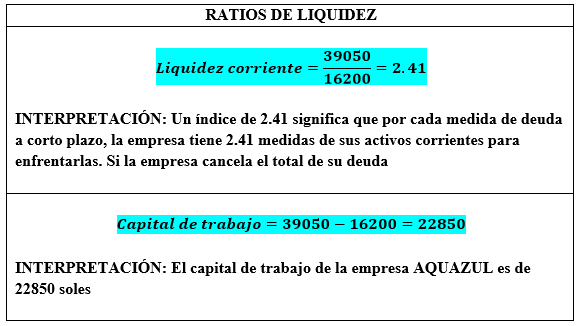
\includegraphics[keepaspectratio]{index_files/figure-html/lu137401d6rd_tmp_c72dfef1.png}}

}

\end{figure}%

\subsubsection{Ratios de gestión}\label{ratios-de-gestiuxf3n}

\begin{figure}[H]

\caption{Análisis de las ratios de gestión.}

{\centering \pandocbounded{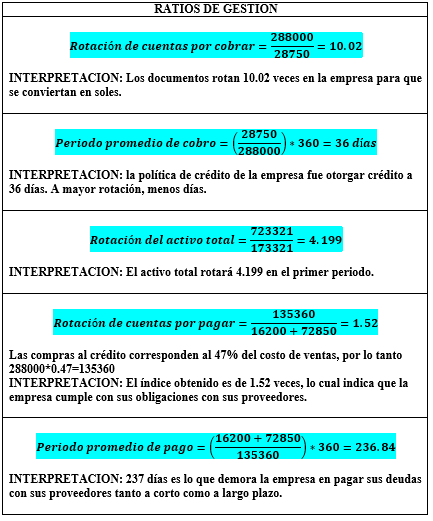
\includegraphics[keepaspectratio]{index_files/figure-html/lu137401d6rd_tmp_52100eb7.png}}

}

\end{figure}%

\subsubsection{Ratios de endeudamiento}\label{ratios-de-endeudamiento}

\begin{figure}[H]

\caption{Análisis de ratios de endeudamiento.}

{\centering \pandocbounded{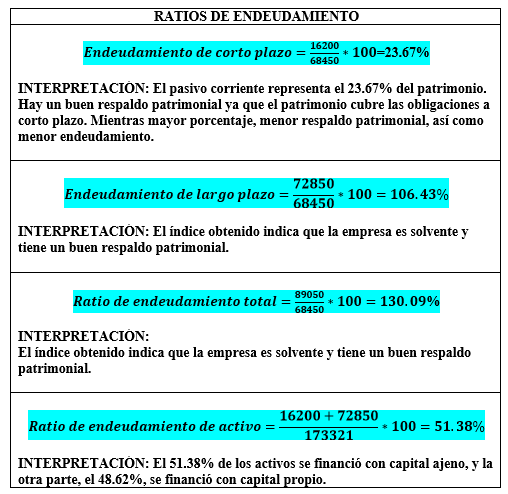
\includegraphics[keepaspectratio]{index_files/figure-html/lu137401d6rd_tmp_ce18a631.png}}

}

\end{figure}%

\subsubsection{Ratios de rentabilidad}\label{ratios-de-rentabilidad}

\begin{figure}[H]

\caption{Análisis de ratios de endeudamiento.}

{\centering \pandocbounded{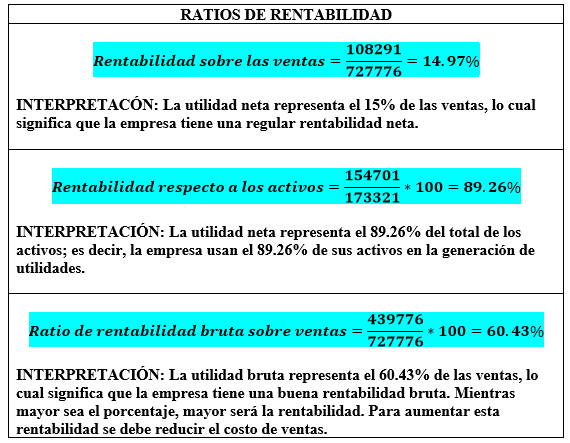
\includegraphics[keepaspectratio]{index_files/figure-html/lu137401d6rd_tmp_2860c5a4.png}}

}

\end{figure}%

\subsection{Plan financiero}\label{plan-financiero}

\subsubsection{Presupuesto maestro}\label{presupuesto-maestro}

\paragraph{Presupuesto de operación.}\label{presupuesto-de-operaciuxf3n}

\textbf{Presupuesto de Ingresos -- Ventas}

\begin{longtable}[]{@{}
  >{\raggedright\arraybackslash}p{(\linewidth - 10\tabcolsep) * \real{0.3000}}
  >{\centering\arraybackslash}p{(\linewidth - 10\tabcolsep) * \real{0.1400}}
  >{\centering\arraybackslash}p{(\linewidth - 10\tabcolsep) * \real{0.1400}}
  >{\centering\arraybackslash}p{(\linewidth - 10\tabcolsep) * \real{0.1400}}
  >{\centering\arraybackslash}p{(\linewidth - 10\tabcolsep) * \real{0.1400}}
  >{\centering\arraybackslash}p{(\linewidth - 10\tabcolsep) * \real{0.1400}}@{}}
\caption{Presupuesto de Ingresos y Ventas}\tabularnewline
\toprule\noalign{}
\begin{minipage}[b]{\linewidth}\raggedright
\textbf{Concepto}
\end{minipage} & \begin{minipage}[b]{\linewidth}\centering
\textbf{Periodo 1}
\end{minipage} & \begin{minipage}[b]{\linewidth}\centering
\textbf{Periodo 2}
\end{minipage} & \begin{minipage}[b]{\linewidth}\centering
\textbf{Periodo 3}
\end{minipage} & \begin{minipage}[b]{\linewidth}\centering
\textbf{Periodo 4}
\end{minipage} & \begin{minipage}[b]{\linewidth}\centering
\textbf{Periodo 5}
\end{minipage} \\
\midrule\noalign{}
\endfirsthead
\toprule\noalign{}
\begin{minipage}[b]{\linewidth}\raggedright
\textbf{Concepto}
\end{minipage} & \begin{minipage}[b]{\linewidth}\centering
\textbf{Periodo 1}
\end{minipage} & \begin{minipage}[b]{\linewidth}\centering
\textbf{Periodo 2}
\end{minipage} & \begin{minipage}[b]{\linewidth}\centering
\textbf{Periodo 3}
\end{minipage} & \begin{minipage}[b]{\linewidth}\centering
\textbf{Periodo 4}
\end{minipage} & \begin{minipage}[b]{\linewidth}\centering
\textbf{Periodo 5}
\end{minipage} \\
\midrule\noalign{}
\endhead
\bottomrule\noalign{}
\endlastfoot
Unidades vendidas & 24000 & 25200 & 26460 & 27783 & 29172.15 \\
Precio Unidad (US\$) & 8.4 & 8.4 & 8.4 & 8.4 & 8.4 \\
Total, ingresos en dólares & 201,600.00 & 211,680.00 & 222,264.00 &
233,377.20 & 245,046.06 \\
\textbf{Total, ingresos en soles} & \textbf{55844.87535} &
\textbf{58637.11911} & \textbf{61568.97507} & \textbf{64647.42382} &
\textbf{67879.795} \\
\end{longtable}

Para la venta del año 1 el ingreso es de S/55844.87535 lo cual se
muestra en la tabla \ldots de 24000 unidades de filete de trucha
refrigerada cada una con 1kg, la que se comercializará a un precio (FCA)
de \$8.40 dólares o S/ 26.54/ unidades, Para los años posteriores los
ingresos se incrementan en 5\%, lo cual es muy favorable para que la
empresa continúe en el mercado dado que las preferencias por el filete
de trucha refrigerada en el mercado estadounidense van incrementando.

\textbf{Presupuesto de Producción}

\begin{longtable}[]{@{}
  >{\raggedright\arraybackslash}p{(\linewidth - 10\tabcolsep) * \real{0.3000}}
  >{\centering\arraybackslash}p{(\linewidth - 10\tabcolsep) * \real{0.1400}}
  >{\centering\arraybackslash}p{(\linewidth - 10\tabcolsep) * \real{0.1400}}
  >{\centering\arraybackslash}p{(\linewidth - 10\tabcolsep) * \real{0.1400}}
  >{\centering\arraybackslash}p{(\linewidth - 10\tabcolsep) * \real{0.1400}}
  >{\centering\arraybackslash}p{(\linewidth - 10\tabcolsep) * \real{0.1400}}@{}}
\caption{Presupuesto de Costos de Producción}\tabularnewline
\toprule\noalign{}
\begin{minipage}[b]{\linewidth}\raggedright
\textbf{CONCEPTO}
\end{minipage} & \begin{minipage}[b]{\linewidth}\centering
\textbf{AÑOS}
\end{minipage} & \begin{minipage}[b]{\linewidth}\centering
\end{minipage} & \begin{minipage}[b]{\linewidth}\centering
\end{minipage} & \begin{minipage}[b]{\linewidth}\centering
\end{minipage} & \begin{minipage}[b]{\linewidth}\centering
\end{minipage} \\
\midrule\noalign{}
\endfirsthead
\toprule\noalign{}
\begin{minipage}[b]{\linewidth}\raggedright
\textbf{CONCEPTO}
\end{minipage} & \begin{minipage}[b]{\linewidth}\centering
\textbf{AÑOS}
\end{minipage} & \begin{minipage}[b]{\linewidth}\centering
\end{minipage} & \begin{minipage}[b]{\linewidth}\centering
\end{minipage} & \begin{minipage}[b]{\linewidth}\centering
\end{minipage} & \begin{minipage}[b]{\linewidth}\centering
\end{minipage} \\
\midrule\noalign{}
\endhead
\bottomrule\noalign{}
\endlastfoot
& \textbf{1} & \textbf{2} & \textbf{3} & \textbf{4} & \textbf{5} \\
\textbf{I. Costos directos} & \textbf{339.050,00} & \textbf{357.327,50}
& \textbf{374.943,88} & \textbf{393.441,07} & \textbf{412.863,12} \\
Compra de trucha al por mayor & 300.000,00 & 315.000,00 & 330.750,00 &
347.287,50 & 364.651,88 \\
Compra de hielo en escamas & 1.050,00 & 1.102,50 & 1.157,63 & 1.215,51 &
1.276,28 \\
Bolsas para empaques con impresión & 2.000,00 & 2.100,00 & 2.205,00 &
2.315,25 & 2.431,01 \\
Mano de obra directa & 32.500,00 & 34.125,00 & 35.831,25 & 37.622,81 &
39.503,95 \\
Otros costos directos & 3.500,00 & 5.000,00 & 5.000,00 & 5.000,00 &
5.000,00 \\
\textbf{II. Costos indirectos} & \textbf{21.080,00} & \textbf{22.134,00}
& \textbf{23.240,70} & \textbf{24.402,74} & \textbf{25.622,87} \\
Mano de obra indirecta & 10.680,00 & 11.214,00 & 11.774,70 & 12.363,44 &
12.981,61 \\
Otros costos indirectos & 10.400,00 & 10.920,00 & 11.466,00 & 12.039,30
& 12.641,27 \\
\textbf{Total de costos de producción} & \textbf{360.130,00} &
\textbf{379.461,50} & \textbf{398.184,58} & \textbf{417.843,80} &
\textbf{438.485,99} \\
\end{longtable}

La tabla 6.11, indica los costos de producción anuales, muestra el
presupuesto de producción mensual para el año 1, en la que se han
considerado los siguientes ítems: costos directos y costos indirectos
dando como resultado el costo total que es la suma de todos los gastos
en los que la empresa piscicola Aquazul S.C.R.L incurre para producir y
comercializar el producto en el mercado estadounidense. Aquí no existen
inventarios puesto que es producto perecible y en cuanto se produce se
comercializa al mercado estadounidense.

Para la compra de materia prima la empresa necesita disponer de S/
303050.00 anuales la que incluye la compra de trucha al por mayor,
compra de hielo en escamas, bolsas para empaques con impresión; para el
pago de la mano de obra directa lo que incluye los trabajadores
encargados de filetear eviscerar, empacar, lavar el producto y dejarlo
listo para ser comercializado se requiere de S/ 32.500,00 anuales , para
los otros costos directos se necesitarán S/ 3.500,00 siendo así la suma
total de costos directos de S/ 339.050,00.

Acerca de los costos indirectos S/ 21.080,00 que es lo que se necesita
para cancelar el sueldo del personal de limpieza, gastos de luz y agua.
Para que la empresa piscicola Aquazul S.C.R.L pueda realizar la
comercialización con el mercado estadounidense necesita disponer de S/
360.130,00 Nuevos soles en el primer año.

\textbf{Presupuesto de gasto de Fabricación}

\begin{longtable}[]{@{}
  >{\raggedright\arraybackslash}p{(\linewidth - 10\tabcolsep) * \real{0.3000}}
  >{\centering\arraybackslash}p{(\linewidth - 10\tabcolsep) * \real{0.1400}}
  >{\centering\arraybackslash}p{(\linewidth - 10\tabcolsep) * \real{0.1400}}
  >{\centering\arraybackslash}p{(\linewidth - 10\tabcolsep) * \real{0.1400}}
  >{\centering\arraybackslash}p{(\linewidth - 10\tabcolsep) * \real{0.1400}}
  >{\centering\arraybackslash}p{(\linewidth - 10\tabcolsep) * \real{0.1400}}@{}}
\caption{Presupuesto de Gasto de Fabricación}\tabularnewline
\toprule\noalign{}
\begin{minipage}[b]{\linewidth}\raggedright
\textbf{Concepto}
\end{minipage} & \begin{minipage}[b]{\linewidth}\centering
\textbf{Periodo 1}
\end{minipage} & \begin{minipage}[b]{\linewidth}\centering
\textbf{Periodo 2}
\end{minipage} & \begin{minipage}[b]{\linewidth}\centering
\textbf{Periodo 3}
\end{minipage} & \begin{minipage}[b]{\linewidth}\centering
\textbf{Periodo 4}
\end{minipage} & \begin{minipage}[b]{\linewidth}\centering
\textbf{Periodo 5}
\end{minipage} \\
\midrule\noalign{}
\endfirsthead
\toprule\noalign{}
\begin{minipage}[b]{\linewidth}\raggedright
\textbf{Concepto}
\end{minipage} & \begin{minipage}[b]{\linewidth}\centering
\textbf{Periodo 1}
\end{minipage} & \begin{minipage}[b]{\linewidth}\centering
\textbf{Periodo 2}
\end{minipage} & \begin{minipage}[b]{\linewidth}\centering
\textbf{Periodo 3}
\end{minipage} & \begin{minipage}[b]{\linewidth}\centering
\textbf{Periodo 4}
\end{minipage} & \begin{minipage}[b]{\linewidth}\centering
\textbf{Periodo 5}
\end{minipage} \\
\midrule\noalign{}
\endhead
\bottomrule\noalign{}
\endlastfoot
TOTAL, INGRESOS & 59874360.98 & 62868079.03 & 69312057.13 & 72777659.99
& 76416542.99 \\
GASTOS ADMINISTRATIVOS & 78,000.00 & 81900 & 85995 & 90294.75 &
94809.4875 \\
GASTOS GENERALES (5\% IF) & 30,430.00 & 31951.5 & 33549.075 &
35226.52875 & 36987.85519 \\
GASTOS DE SUPERVISIÓN (3\% IF) & 18,258.00 & 19170.9 & 20129.445 &
21135.91725 & 22192.71311 \\
\textbf{TOTAL, COSTOS INDIRECTOS DE FABRICACIÓN} & \textbf{126,688.00} &
\textbf{133022.4} & \textbf{139673.52} & \textbf{146657.196} &
\textbf{153990.0558} \\
\end{longtable}

La tabla 6.12. muestra los gastos de fabricación en los que incurrirá la
empresa, ello a sido proyectado para hasta el periodo 5,

Siendo para el primer año estos gastos de fabricación los siguientes
gastos administrativos el cual tiene como monto S/78,000.00 soles
anules, gastos generales S/30,430.00, gastos de supervisión S/ 18,258.00
siendo así el total de los costos indirectos de fabricación S/126,688.00
anuales.

\paragraph{Presupuesto de
construcción.}\label{presupuesto-de-construcciuxf3n}

\begin{table}

{\caption{{Presupuesto de construcción para la planta
procesadora}{\label{tbl-mytable2-apa-notediario-el-peruano-valores-unitarios-data-quarto-disable-processingtrue-tbl-colwidths221422141414}}}}

\begin{longtable}[]{@{}
  >{\raggedright\arraybackslash}p{(\linewidth - 10\tabcolsep) * \real{0.1667}}
  >{\centering\arraybackslash}p{(\linewidth - 10\tabcolsep) * \real{0.1667}}
  >{\raggedright\arraybackslash}p{(\linewidth - 10\tabcolsep) * \real{0.1667}}
  >{\centering\arraybackslash}p{(\linewidth - 10\tabcolsep) * \real{0.1667}}
  >{\centering\arraybackslash}p{(\linewidth - 10\tabcolsep) * \real{0.1667}}
  >{\centering\arraybackslash}p{(\linewidth - 10\tabcolsep) * \real{0.1667}}@{}}
\toprule\noalign{}
\begin{minipage}[b]{\linewidth}\raggedright
\textbf{Item Construcción}
\end{minipage} & \begin{minipage}[b]{\linewidth}\centering
\textbf{Unidad De Medida}
\end{minipage} & \begin{minipage}[b]{\linewidth}\raggedright
\textbf{Especificación Técnica}
\end{minipage} & \begin{minipage}[b]{\linewidth}\centering
\textbf{Tamaño}
\end{minipage} & \begin{minipage}[b]{\linewidth}\centering
\textbf{Costo Unitario}
\end{minipage} & \begin{minipage}[b]{\linewidth}\centering
\textbf{Costo Total}
\end{minipage} \\
\midrule\noalign{}
\endhead
\bottomrule\noalign{}
\endlastfoot
Terreno & m2 & Terreno para la construcción & 140 m2 & 50 & 7000 \\
\textbf{ESTRUCTURAS} & & & & & \\
Muro de ladrillo & m2 & Ladrillo & 140 m2 & 207 & 28980 \\
Techo & m2 & Estructura metálica & 140 m2 & 88 & 12320 \\
Piso & m2 & Concreto & 140 m2 & 57 & 7980 \\
\textbf{ACABADOS} & & & & & \\
Portón & m2 & Metal & 12 m2 & 132 & 1585 \\
Baños & m2 & Cerámica & 12 m2 & 26 & 312 \\
Instalaciones eléctricas y sanitarias & m2 & Sistema de corriente y agua
& 140 m2 & 74 & 10329 \\
Instalación de tanque elevado. & m3 & Sistema de agua & 140 m2 & 634 &
634 \\
Revestimientos & m2 & Tarrajeo y pintado & 140 m2 & 65 & 9100 \\
\textbf{TOTAL, DE CONSTRUCCIONES} & & & & & \textbf{78240} \\
\end{longtable}

\end{table}

La tabla 6.13. muestra el total de inversiones para la construcción de
la planta procesadora de filete de trucha la que asciende a S/ 78239,
valores tomados de el diario Oficial ``El Peruano'' en el que se
detallan los costos unitarios para la construcción teniendo en cuenta el
material a utilizar, la tabla también muestra el costo del terreno
ubicado en la Asociación José Ortiz Vergara que asciende a S/ 101000.00
los 140 M2.

\paragraph{Presupuesto de maquinaria y
equipo.}\label{presupuesto-de-maquinaria-y-equipo}

\begin{longtable}[]{@{}
  >{\raggedright\arraybackslash}p{(\linewidth - 6\tabcolsep) * \real{0.4265}}
  >{\centering\arraybackslash}p{(\linewidth - 6\tabcolsep) * \real{0.1471}}
  >{\centering\arraybackslash}p{(\linewidth - 6\tabcolsep) * \real{0.2353}}
  >{\centering\arraybackslash}p{(\linewidth - 6\tabcolsep) * \real{0.1912}}@{}}
\caption{Presupuesto de maquinaria para el funcionamiento de la planta
procesadora de filete de trucha para producir 10 TM}\tabularnewline
\toprule\noalign{}
\begin{minipage}[b]{\linewidth}\raggedright
Descripción
\end{minipage} & \begin{minipage}[b]{\linewidth}\centering
Cantidad
\end{minipage} & \begin{minipage}[b]{\linewidth}\centering
Costo unitario
\end{minipage} & \begin{minipage}[b]{\linewidth}\centering
Costo total
\end{minipage} \\
\midrule\noalign{}
\endfirsthead
\toprule\noalign{}
\begin{minipage}[b]{\linewidth}\raggedright
Descripción
\end{minipage} & \begin{minipage}[b]{\linewidth}\centering
Cantidad
\end{minipage} & \begin{minipage}[b]{\linewidth}\centering
Costo unitario
\end{minipage} & \begin{minipage}[b]{\linewidth}\centering
Costo total
\end{minipage} \\
\midrule\noalign{}
\endhead
\bottomrule\noalign{}
\endlastfoot
Armario de refrigeración & 1 & 52800 & 52800 \\
Máquina de empaque al vacío & 1 & 5749 & 5749 \\
Mesas de metal & 6 & 480 & 2880 \\
Jabas para pescado x 25 kg & 34 & 10 & 340 \\
Tinas de metal & 6 & 25 & 150 \\
Balanzas & 2 & 490 & 980 \\
& & & \textbf{62899} \\
\end{longtable}

La tabla 6.14 muestra el total de inversiones para la adquisición de
maquinaria requerida para llevar a cabo el proyecto la que asciende a S/
62899, en la que se va a comprar un armario de refrigeración para la
conservación del producto, maquinaria de empaque al vacío para sellar el
producto, mesas de metal necesarias para el proceso requerido, jabas de
pescado para su transporte de un lugar a otro, tinas de metal para su
almacenamiento y balanzas para el pesado de nuestro producto.

\subsubsection{Crédito bancario}\label{cruxe9dito-bancario}

\begin{longtable}[]{@{}lcc@{}}
\caption{Capital Total para emprender el Proyecto}\tabularnewline
\toprule\noalign{}
Construcción & 78240.00 & \\
\midrule\noalign{}
\endfirsthead
\toprule\noalign{}
Construcción & 78240.00 & \\
\midrule\noalign{}
\endhead
\bottomrule\noalign{}
\endlastfoot
Equipos & 62899.00 & \\
TOTAL, PARA EJECUTAR PROYECTO & 141139.00 & \\
Inversionistas & 24\% & 34000 \\
Financiamiento & 76\% & 107139.00 \\
\end{longtable}

Para saber cuánto será la tasa de interés y las cuotas que se van a
pagar mensualmente a la entidad financiera se ha recurrido a un
simulador de créditos de la Financiera ProEmpresa, en cual se muestra a
partir del siguiente gráfico.

\begin{figure}[H]

\caption{Simulador de Crédito Simulador de Crédito}

{\centering \pandocbounded{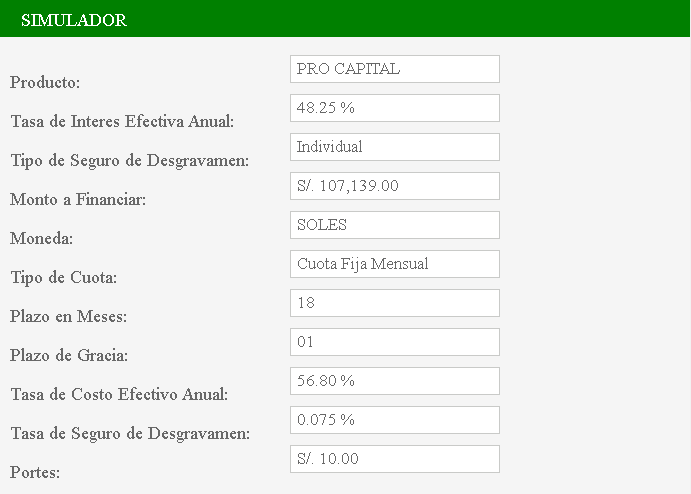
\includegraphics[keepaspectratio]{index_files/figure-html/lu137401d6rd_tmp_1842ef6a.png}}

}

\end{figure}%

Fuente: Elaboración Propia, a partir del simulador de crédito ProEmpresa

En base a la información anterior se realiza los siguientes cálculos:
Intereses, amortización y cuota

\begin{table}

{\caption{{Tabla de Amortizaciones}{\label{tbl-mytable2}}}}

\begin{longtable}[]{@{}lccc@{}}
\toprule\noalign{}
CAPITAL & 107,139.00 & & \\
\midrule\noalign{}
\endhead
\bottomrule\noalign{}
\endlastfoot
TEM & 3.34\% & & \\
AÑOS & 5.0 & & \\
FRECUENCIA & 1 & & \\
NÚMERO DE PAGOS & 5 & & \\
\textbf{PERIODO} & \textbf{INTERESES} & \textbf{AMORTIZACIÓN} &
\textbf{CUOTA} \\
1 & S/51,694.57 & S/8,390.62 & S/60,085.18 \\
2 & S/47,646.09 & S/12,439.09 & S/60,085.18 \\
3 & S/41,644.23 & S/18,440.95 & S/60,085.18 \\
4 & S/32,746.48 & S/27,338.71 & S/60,085.18 \\
5 & S/19,555.55 & S/40,529.64 & S/60,085.18 \\
\end{longtable}

{\noindent \emph{Note.} Elaboración Propia, a partir del simulador de crédito ProEmpresa}

\end{table}

Para llevar a cabo el proyecto se necesita una inversión total de
S/107139.00, que será financiada con el 76\% con un préstamo otorgado
por la entidad financiera ProEmpresa cuyo monto asciende a S/107139.00,
el cual será cancelado en 5años.

Donde: El Valor de cuota es de 8,012.57, con una TEA de 48.25 \% y una
TEM de 3.34\%

\subsubsection{Presupuesto de gastos (administrativos, exportación y
financieros)}\label{presupuesto-de-gastos-administrativos-exportaciuxf3n-y-financieros}

\begin{longtable}[]{@{}
  >{\raggedright\arraybackslash}p{(\linewidth - 10\tabcolsep) * \real{0.3000}}
  >{\centering\arraybackslash}p{(\linewidth - 10\tabcolsep) * \real{0.1400}}
  >{\centering\arraybackslash}p{(\linewidth - 10\tabcolsep) * \real{0.1400}}
  >{\centering\arraybackslash}p{(\linewidth - 10\tabcolsep) * \real{0.1400}}
  >{\centering\arraybackslash}p{(\linewidth - 10\tabcolsep) * \real{0.1400}}
  >{\centering\arraybackslash}p{(\linewidth - 10\tabcolsep) * \real{0.1400}}@{}}
\caption{Gastos administrativos para los años del 1 al 5}\tabularnewline
\toprule\noalign{}
\begin{minipage}[b]{\linewidth}\raggedright
\textbf{CONCEPTO}
\end{minipage} & \begin{minipage}[b]{\linewidth}\centering
\textbf{1}
\end{minipage} & \begin{minipage}[b]{\linewidth}\centering
\textbf{2}
\end{minipage} & \begin{minipage}[b]{\linewidth}\centering
\textbf{3}
\end{minipage} & \begin{minipage}[b]{\linewidth}\centering
\textbf{4}
\end{minipage} & \begin{minipage}[b]{\linewidth}\centering
\textbf{5}
\end{minipage} \\
\midrule\noalign{}
\endfirsthead
\toprule\noalign{}
\begin{minipage}[b]{\linewidth}\raggedright
\textbf{CONCEPTO}
\end{minipage} & \begin{minipage}[b]{\linewidth}\centering
\textbf{1}
\end{minipage} & \begin{minipage}[b]{\linewidth}\centering
\textbf{2}
\end{minipage} & \begin{minipage}[b]{\linewidth}\centering
\textbf{3}
\end{minipage} & \begin{minipage}[b]{\linewidth}\centering
\textbf{4}
\end{minipage} & \begin{minipage}[b]{\linewidth}\centering
\textbf{5}
\end{minipage} \\
\midrule\noalign{}
\endhead
\bottomrule\noalign{}
\endlastfoot
Sueldo administrativo & 74400 & 74400 & 74400 & 74400 & 74400 \\
Promoción y publicidad & 8733 & 8733 & 8733 & 8733 & 8733 \\
Otros Gastos adm. & 3600 & 3600 & 3600 & 3600 & 3600 \\
\textbf{Total Gastos Adm.} & \textbf{86733} & \textbf{86733} &
\textbf{86733} & \textbf{86733} & \textbf{86733} \\
\end{longtable}

La tabla 6.17., muestra los gastos administrativos para los años 1 al 5,
en los que se ha considerado el sueldo para el personal administrativo,
pero aquí no se considera el Sueldo del jefe de producción qué es
considerado como mano de obra directa, en la tabla de producción;
también se consideran los gastos por teléfonos e internet, así como los
gastos de promoción y publicidad descrita en el plan de marketing,
dichos gastos son de 86733 anuales necesarios para cancelar los gastos
administrativos.

\begin{longtable}[]{@{}
  >{\raggedright\arraybackslash}p{(\linewidth - 10\tabcolsep) * \real{0.3000}}
  >{\centering\arraybackslash}p{(\linewidth - 10\tabcolsep) * \real{0.1400}}
  >{\centering\arraybackslash}p{(\linewidth - 10\tabcolsep) * \real{0.1400}}
  >{\centering\arraybackslash}p{(\linewidth - 10\tabcolsep) * \real{0.1400}}
  >{\centering\arraybackslash}p{(\linewidth - 10\tabcolsep) * \real{0.1400}}
  >{\centering\arraybackslash}p{(\linewidth - 10\tabcolsep) * \real{0.1400}}@{}}
\caption{Gastos de exportación
\{apa-note=\textquotesingle SANIPES\textquotesingle{}
data-quarto-disable-processing=\textquotesingle true\textquotesingle\}}\tabularnewline
\toprule\noalign{}
\begin{minipage}[b]{\linewidth}\raggedright
\textbf{CONCEPTOS}
\end{minipage} & \begin{minipage}[b]{\linewidth}\centering
\textbf{1}
\end{minipage} & \begin{minipage}[b]{\linewidth}\centering
\textbf{2}
\end{minipage} & \begin{minipage}[b]{\linewidth}\centering
\textbf{3}
\end{minipage} & \begin{minipage}[b]{\linewidth}\centering
\textbf{4}
\end{minipage} & \begin{minipage}[b]{\linewidth}\centering
\textbf{5}
\end{minipage} \\
\midrule\noalign{}
\endfirsthead
\toprule\noalign{}
\begin{minipage}[b]{\linewidth}\raggedright
\textbf{CONCEPTOS}
\end{minipage} & \begin{minipage}[b]{\linewidth}\centering
\textbf{1}
\end{minipage} & \begin{minipage}[b]{\linewidth}\centering
\textbf{2}
\end{minipage} & \begin{minipage}[b]{\linewidth}\centering
\textbf{3}
\end{minipage} & \begin{minipage}[b]{\linewidth}\centering
\textbf{4}
\end{minipage} & \begin{minipage}[b]{\linewidth}\centering
\textbf{5}
\end{minipage} \\
\midrule\noalign{}
\endhead
\bottomrule\noalign{}
\endlastfoot
Empaque / embalaje & 17761 & 32148 & 58187 & 105319 & 190628 \\
Terminal aéreo & 223 & 223 & 223 & 223 & 223 \\
Costos aduaneros & 13862 & 13862 & 13862 & 13862 & 13862 \\
AWB & 116 & 116 & 116 & 116 & 116 \\
Transporte local & 251 & 251 & 251 & 251 & 251 \\
Transporte internacional & 207187 & 207187 & 207187 & 207187 & 207187 \\
Seguro & 0 & 0 & 0 & 0 & 0 \\
Certificados & 4583 & 4583 & 4583 & 4583 & 4583 \\
\textbf{Total g. Exportación} & \textbf{243983} & \textbf{258369} &
\textbf{284409} & \textbf{331541} & \textbf{416850} \\
\end{longtable}

La tabla 6.18, muestra los gastos de exportación en los que se considera
el empaque y embalaje; así como los costos aduaneros que se consideran
en el análisis de precios de exportación, los que se necesita cubrir con
una cantidad de 243983, en el que va incrementando año a año 0.81\% De
acuerdo con la tasa de crecimiento poblacional en Estados Unidos.

\begin{longtable}[]{@{}
  >{\raggedright\arraybackslash}p{(\linewidth - 10\tabcolsep) * \real{0.3000}}
  >{\centering\arraybackslash}p{(\linewidth - 10\tabcolsep) * \real{0.1400}}
  >{\centering\arraybackslash}p{(\linewidth - 10\tabcolsep) * \real{0.1400}}
  >{\centering\arraybackslash}p{(\linewidth - 10\tabcolsep) * \real{0.1400}}
  >{\centering\arraybackslash}p{(\linewidth - 10\tabcolsep) * \real{0.1400}}
  >{\centering\arraybackslash}p{(\linewidth - 10\tabcolsep) * \real{0.1400}}@{}}
\caption{Gastos Financieros}\tabularnewline
\toprule\noalign{}
\begin{minipage}[b]{\linewidth}\raggedright
\textbf{CONCEPTO}
\end{minipage} & \begin{minipage}[b]{\linewidth}\centering
\textbf{1}
\end{minipage} & \begin{minipage}[b]{\linewidth}\centering
\textbf{2}
\end{minipage} & \begin{minipage}[b]{\linewidth}\centering
\textbf{3}
\end{minipage} & \begin{minipage}[b]{\linewidth}\centering
\textbf{4}
\end{minipage} & \begin{minipage}[b]{\linewidth}\centering
\textbf{5}
\end{minipage} \\
\midrule\noalign{}
\endfirsthead
\toprule\noalign{}
\begin{minipage}[b]{\linewidth}\raggedright
\textbf{CONCEPTO}
\end{minipage} & \begin{minipage}[b]{\linewidth}\centering
\textbf{1}
\end{minipage} & \begin{minipage}[b]{\linewidth}\centering
\textbf{2}
\end{minipage} & \begin{minipage}[b]{\linewidth}\centering
\textbf{3}
\end{minipage} & \begin{minipage}[b]{\linewidth}\centering
\textbf{4}
\end{minipage} & \begin{minipage}[b]{\linewidth}\centering
\textbf{5}
\end{minipage} \\
\midrule\noalign{}
\endhead
\bottomrule\noalign{}
\endlastfoot
Intereses & 51695 & 47646 & 41644 & 32746 & 19556 \\
Amortizaciones & 8391 & 12439 & 18441 & 27339 & 40530 \\
\textbf{Total de gastos financieros} & \textbf{60085} & \textbf{60085} &
\textbf{60085} & \textbf{60085} & \textbf{60085} \\
\end{longtable}

La tabla 6.19., muestra los gastos financieros para los años proyectados
luz que ascienden a 60085 para el primer año, donde las amortizaciones
van incrementando y a lo largo del proyecto lo que demuestra que el
préstamo sí está cancelando año tras año, Por otro lado los intereses
generados por el préstamo adquirido pan disminuyendo en cuanto se va
cancelando el préstamo para llevar a cabo el proyecto.

\subsubsection{Presupuesto financiero}\label{presupuesto-financiero}

\begin{longtable}[]{@{}
  >{\raggedright\arraybackslash}p{(\linewidth - 10\tabcolsep) * \real{0.3000}}
  >{\centering\arraybackslash}p{(\linewidth - 10\tabcolsep) * \real{0.1400}}
  >{\centering\arraybackslash}p{(\linewidth - 10\tabcolsep) * \real{0.1400}}
  >{\centering\arraybackslash}p{(\linewidth - 10\tabcolsep) * \real{0.1400}}
  >{\centering\arraybackslash}p{(\linewidth - 10\tabcolsep) * \real{0.1400}}
  >{\centering\arraybackslash}p{(\linewidth - 10\tabcolsep) * \real{0.1400}}@{}}
\caption{Estado de resultados con financiamiento}\tabularnewline
\toprule\noalign{}
\begin{minipage}[b]{\linewidth}\raggedright
\textbf{CONCEPTO}
\end{minipage} & \begin{minipage}[b]{\linewidth}\centering
\textbf{1}
\end{minipage} & \begin{minipage}[b]{\linewidth}\centering
\textbf{2}
\end{minipage} & \begin{minipage}[b]{\linewidth}\centering
\textbf{3}
\end{minipage} & \begin{minipage}[b]{\linewidth}\centering
\textbf{4}
\end{minipage} & \begin{minipage}[b]{\linewidth}\centering
\textbf{5}
\end{minipage} \\
\midrule\noalign{}
\endfirsthead
\toprule\noalign{}
\begin{minipage}[b]{\linewidth}\raggedright
\textbf{CONCEPTO}
\end{minipage} & \begin{minipage}[b]{\linewidth}\centering
\textbf{1}
\end{minipage} & \begin{minipage}[b]{\linewidth}\centering
\textbf{2}
\end{minipage} & \begin{minipage}[b]{\linewidth}\centering
\textbf{3}
\end{minipage} & \begin{minipage}[b]{\linewidth}\centering
\textbf{4}
\end{minipage} & \begin{minipage}[b]{\linewidth}\centering
\textbf{5}
\end{minipage} \\
\midrule\noalign{}
\endhead
\bottomrule\noalign{}
\endlastfoot
Ventas & 727776 & 733671 & 739614 & 745605 & 751644 \\
Costo de ventas & 288000 & 290333 & 292684 & 295055 & 297445 \\
Utilidad bruta & 439776 & 443338 & 446929 & 450549 & 454199 \\
Gastos administrativos & 86733 & 86733 & 86733 & 86733 & 86733 \\
Gastos de venta & 49656 & 49656 & 49656 & 49656 & 49656 \\
Depreciación & 12580 & 12580 & 12580 & 12580 & 12580 \\
Amortización & 8391 & 12439 & 18441 & 27339 & 40530 \\
Utilidad de la operación & 282416 & 281930 & 279519 & 274242 & 264700 \\
Gastos financieros & 60085 & 60085 & 60085 & 60085 & 60085 \\
Utilidad antes de impuestos & 222331 & 221845 & 219434 & 214156 &
204615 \\
Impuesto Renta & 66699 & 66553 & 65830 & 64247 & 61384 \\
\textbf{Utilidad neta} & \textbf{155632} & \textbf{155291} &
\textbf{153604} & \textbf{149909} & \textbf{143230} \\
\end{longtable}

La tabla denominada estado resultados sin financiamiento muestra que al
finalizar el periodo la empresa obtiene una utilidad que proyectada a
través del tiempo va incrementando, mostrando un resultado favorable
para la empresa. Mientras que una variación promedio de 11\% durante los
5 años considerados para el proyecto. Este resultado nos muestra que la
participación en ventas los filetes de trucha arcoíris en el mercado
estadounidense es positiva.

\subsubsection{Análisis de
rentabilidad}\label{anuxe1lisis-de-rentabilidad}

Para poder realizar el análisis de rentabilidad hacemos uso del flujo de
caja el cual nos permite ingresar en el análisis del VAN y TIR para
poder diagnosticar la rentabilidad del negocio.

\begin{longtable}[]{@{}
  >{\raggedright\arraybackslash}p{(\linewidth - 12\tabcolsep) * \real{0.2600}}
  >{\centering\arraybackslash}p{(\linewidth - 12\tabcolsep) * \real{0.1200}}
  >{\centering\arraybackslash}p{(\linewidth - 12\tabcolsep) * \real{0.1200}}
  >{\centering\arraybackslash}p{(\linewidth - 12\tabcolsep) * \real{0.1200}}
  >{\centering\arraybackslash}p{(\linewidth - 12\tabcolsep) * \real{0.1200}}
  >{\centering\arraybackslash}p{(\linewidth - 12\tabcolsep) * \real{0.1200}}
  >{\centering\arraybackslash}p{(\linewidth - 12\tabcolsep) * \real{0.1200}}@{}}
\caption{Flujo de caja proyectado sin financiamiento}\tabularnewline
\toprule\noalign{}
\begin{minipage}[b]{\linewidth}\raggedright
CONCEPTOS
\end{minipage} & \begin{minipage}[b]{\linewidth}\centering
\textbf{0}
\end{minipage} & \begin{minipage}[b]{\linewidth}\centering
\textbf{1}
\end{minipage} & \begin{minipage}[b]{\linewidth}\centering
\textbf{2}
\end{minipage} & \begin{minipage}[b]{\linewidth}\centering
\textbf{3}
\end{minipage} & \begin{minipage}[b]{\linewidth}\centering
\textbf{4}
\end{minipage} & \begin{minipage}[b]{\linewidth}\centering
\textbf{5}
\end{minipage} \\
\midrule\noalign{}
\endfirsthead
\toprule\noalign{}
\begin{minipage}[b]{\linewidth}\raggedright
CONCEPTOS
\end{minipage} & \begin{minipage}[b]{\linewidth}\centering
\textbf{0}
\end{minipage} & \begin{minipage}[b]{\linewidth}\centering
\textbf{1}
\end{minipage} & \begin{minipage}[b]{\linewidth}\centering
\textbf{2}
\end{minipage} & \begin{minipage}[b]{\linewidth}\centering
\textbf{3}
\end{minipage} & \begin{minipage}[b]{\linewidth}\centering
\textbf{4}
\end{minipage} & \begin{minipage}[b]{\linewidth}\centering
\textbf{5}
\end{minipage} \\
\midrule\noalign{}
\endhead
\bottomrule\noalign{}
\endlastfoot
\textbf{INGRESOS} & & \textbf{727776} & \textbf{764165} &
\textbf{802373} & \textbf{842492} & \textbf{884616} \\
\textbf{Venta de Activos} & & & & & & \\
Costo Producción & & 273080 & 273080 & 273080 & 273080 & 273080 \\
Gastos Administrativos & & 86733 & 86733 & 86733 & 86733 & 86733 \\
Gastos de Venta & & 49656 & 49656 & 49656 & 49656 & 49656 \\
Depreciación maquinarias & & 7428 & 7428 & 7428 & 7428 & 7428 \\
Depreciación de Construcciones & & 3526 & 3526 & 3526 & 3526 & 3526 \\
Amortización De Intangibles & & 13798,4 & 13798,4 & 13798,4 & 13798,4 &
13798,4 \\
\textbf{Utilidad} & & \textbf{293554} & \textbf{329943} &
\textbf{368151} & \textbf{408270} & \textbf{450395} \\
Renta & & 88066,29 & 98982,93 & 110445,40 & 122480,99 & 135118,37 \\
\textbf{Utilidad Neta} & & \textbf{205488,00} & \textbf{230960,16} &
\textbf{257705,93} & \textbf{285788,99} & \textbf{315276,20} \\
Depreciación Maquinarias & & 7428 & 7428 & 7428 & 7428 & 7428 \\
Depreciación Construcciones & & 3526 & 3526 & 3526 & 3526 & 3526 \\
Equipos (10) & 58317 & & & & & 58317 \\
Equipos (5) & 4386 & & & & & \\
Equipos (1) & 196 & & & & & \\
Intangibles & 68992 & & & & & \\
Amortización De Intangibles & & 13798 & 13798 & 13798 & 13798 & 13798 \\
Terreno & 101000 & & & & & 101000 \\
Construcciones & 78240 & & & & & 60610 \\
Capital Trabajo & 22850 & 69548 & 104015 & 133487 & 207553 & 537453 \\
\textbf{Flujo De Caja} & \textbf{-333981} & \textbf{11450} &
\textbf{148971} & \textbf{151698} & \textbf{160692} &
\textbf{1097409} \\
\end{longtable}

Al realizarse el flujo de caja económico se puede observar que se tiene
un flujo para el primer año S/. 333981, el cual se va incrementando a lo
largo de los años cómo llegando a 1097409 para el quinto año del
proyecto cómo el cual es un resultado positivo y favorable para la
empresa.

\begin{longtable}[]{@{}
  >{\raggedright\arraybackslash}p{(\linewidth - 12\tabcolsep) * \real{0.3100}}
  >{\centering\arraybackslash}p{(\linewidth - 12\tabcolsep) * \real{0.1200}}
  >{\centering\arraybackslash}p{(\linewidth - 12\tabcolsep) * \real{0.1200}}
  >{\centering\arraybackslash}p{(\linewidth - 12\tabcolsep) * \real{0.1200}}
  >{\centering\arraybackslash}p{(\linewidth - 12\tabcolsep) * \real{0.1200}}
  >{\centering\arraybackslash}p{(\linewidth - 12\tabcolsep) * \real{0.1200}}
  >{\centering\arraybackslash}p{(\linewidth - 12\tabcolsep) * \real{0.1200}}@{}}
\caption{Flujo de caja proyectado con financiamiento}\tabularnewline
\toprule\noalign{}
\begin{minipage}[b]{\linewidth}\raggedright
CONCEPTO
\end{minipage} & \begin{minipage}[b]{\linewidth}\centering
\textbf{0}
\end{minipage} & \begin{minipage}[b]{\linewidth}\centering
\textbf{1}
\end{minipage} & \begin{minipage}[b]{\linewidth}\centering
\textbf{2}
\end{minipage} & \begin{minipage}[b]{\linewidth}\centering
\textbf{3}
\end{minipage} & \begin{minipage}[b]{\linewidth}\centering
\textbf{4}
\end{minipage} & \begin{minipage}[b]{\linewidth}\centering
\textbf{5}
\end{minipage} \\
\midrule\noalign{}
\endfirsthead
\toprule\noalign{}
\begin{minipage}[b]{\linewidth}\raggedright
CONCEPTO
\end{minipage} & \begin{minipage}[b]{\linewidth}\centering
\textbf{0}
\end{minipage} & \begin{minipage}[b]{\linewidth}\centering
\textbf{1}
\end{minipage} & \begin{minipage}[b]{\linewidth}\centering
\textbf{2}
\end{minipage} & \begin{minipage}[b]{\linewidth}\centering
\textbf{3}
\end{minipage} & \begin{minipage}[b]{\linewidth}\centering
\textbf{4}
\end{minipage} & \begin{minipage}[b]{\linewidth}\centering
\textbf{5}
\end{minipage} \\
\midrule\noalign{}
\endhead
\bottomrule\noalign{}
\endlastfoot
\textbf{INGRESOS} & & \textbf{727776} & \textbf{764165} &
\textbf{802373} & \textbf{842492} & \textbf{884616} \\
\textbf{Venta de Activos} & & & & & & \\
Costo Producción & & 273080 & 286734 & 301071 & 316124 & 331930 \\
Gastos Administrativos & & 86733 & 86733 & 86733 & 86733 & 86733 \\
Gastos de Venta & & 49656 & 49656 & 49656 & 49656 & 49656 \\
Depreciación de Maquinarias & & 7428 & 7428 & 7428 & 7428 & 7428 \\
Depreciación de Construcciones & & 3526 & 3526 & 3526 & 3526 & 3526 \\
Amortización De Intangibles & & 489 & 489 & 489 & 489 & 489 \\
Intereses/Préstamos & & 25744 & 22545 & 18579 & 13661 & 7562 \\
\textbf{Utilidad} & & \textbf{281120} & \textbf{307053} &
\textbf{334891} & \textbf{364874} & \textbf{397291} \\
Renta & & 84335,98 & 92116,00 & 100467,34 & 109462,33 & 119187,40 \\
\textbf{Utilidad Neta} & & \textbf{196783,95} & \textbf{214937,34} &
\textbf{234423,80} & \textbf{255412,10} & \textbf{278103,94} \\
Depreciación de Maquinarias & & 7428 & 7428 & 7428 & 7428 & 7428 \\
Depreciación Construcciones & & 3526 & 3526 & 3526 & 3526 & 3526 \\
Amortización de la Deuda & & 13328 & 16526 & 20492 & 25411 & 31509 \\
Equipos (10) & 58317 & & & & & 58317 \\
Equipos (5) & 4386 & & & & & \\
Equipos (1) & 196 & 196 & 196 & 196 & 196 & 196 \\
Intangibles & 68992 & & & & & \\
Amortización De Intangibles & & 13798 & 13798 & 13798 & 13798 & 13798 \\
Préstamo & 107266 & & & & & \\
Terreno & 101000 & & & & & 101000 \\
Construcciones & 78240 & & & & & 60610 \\
Capital Trabajo & 22850 & 69548 & 104015 & 133487 & 207553 & 537453 \\
\textbf{Flujo De Caja} & \textbf{-226715} & \textbf{118953} &
\textbf{18139} & \textbf{200585} & \textbf{19456} & \textbf{1021103} \\
\end{longtable}

En realizar el flujo de caja financiero observamos que se tiene un flujo
de 226715 para el primer año cómo al igual que en el flujo de caja
económico, tiene un comportamiento creciente a lo largo de los años
proyectados, resultado favorable para la empresa, ya qué representa el
dinero disponible en caja después de haber pagado todos los costos,
gastos y obligaciones financieras.

\textbf{Evaluación económica-financiera}

\begin{longtable}[]{@{}
  >{\raggedright\arraybackslash}p{(\linewidth - 8\tabcolsep) * \real{0.5571}}
  >{\centering\arraybackslash}p{(\linewidth - 8\tabcolsep) * \real{0.1143}}
  >{\centering\arraybackslash}p{(\linewidth - 8\tabcolsep) * \real{0.1000}}
  >{\centering\arraybackslash}p{(\linewidth - 8\tabcolsep) * \real{0.1000}}
  >{\centering\arraybackslash}p{(\linewidth - 8\tabcolsep) * \real{0.1286}}@{}}
\caption{Evaluación Económica}\tabularnewline
\toprule\noalign{}
\begin{minipage}[b]{\linewidth}\raggedright
COK (Costo de oportunidad de Capital)
\end{minipage} & \begin{minipage}[b]{\linewidth}\centering
0,1594
\end{minipage} & \begin{minipage}[b]{\linewidth}\centering
VANE
\end{minipage} & \begin{minipage}[b]{\linewidth}\centering
90155
\end{minipage} & \begin{minipage}[b]{\linewidth}\centering
\end{minipage} \\
\midrule\noalign{}
\endfirsthead
\toprule\noalign{}
\begin{minipage}[b]{\linewidth}\raggedright
COK (Costo de oportunidad de Capital)
\end{minipage} & \begin{minipage}[b]{\linewidth}\centering
0,1594
\end{minipage} & \begin{minipage}[b]{\linewidth}\centering
VANE
\end{minipage} & \begin{minipage}[b]{\linewidth}\centering
90155
\end{minipage} & \begin{minipage}[b]{\linewidth}\centering
\end{minipage} \\
\midrule\noalign{}
\endhead
\bottomrule\noalign{}
\endlastfoot
& & 15,94 & TIRE & 27.00 \% \\
\end{longtable}

\textbf{Valor Actual neto -- VAN}

Al realizar la evaluación del proyecto sin considerar un financiamiento,
considerando todos los flujos de caja, utilizando una tasa de descuento
del 15\% se recupera la inversión inicial y nos queda un VANE de
S/.90155, lo que demuestra que la empresa obtiene un beneficio por lo
tanto se acepta el proyecto.

\textbf{Tasa interna tu retorno -TIR}

De acuerdo con la evaluación realizada se observa que el proyecto arroja
una tasa de rendimiento de 16\%, considerando un VANE de S/. 90155 por
lo que se afirma que el proyecto es factible.

\begin{longtable}[]{@{}
  >{\raggedright\arraybackslash}p{(\linewidth - 8\tabcolsep) * \real{0.6286}}
  >{\centering\arraybackslash}p{(\linewidth - 8\tabcolsep) * \real{0.0857}}
  >{\centering\arraybackslash}p{(\linewidth - 8\tabcolsep) * \real{0.0857}}
  >{\centering\arraybackslash}p{(\linewidth - 8\tabcolsep) * \real{0.1000}}
  >{\centering\arraybackslash}p{(\linewidth - 8\tabcolsep) * \real{0.1000}}@{}}
\caption{Evaluación financiera}\tabularnewline
\toprule\noalign{}
\begin{minipage}[b]{\linewidth}\raggedright
WACC (Costo Promedio Ponderado de Capital)
\end{minipage} & \begin{minipage}[b]{\linewidth}\centering
0,32
\end{minipage} & \begin{minipage}[b]{\linewidth}\centering
VANF
\end{minipage} & \begin{minipage}[b]{\linewidth}\centering
69518
\end{minipage} & \begin{minipage}[b]{\linewidth}\centering
\end{minipage} \\
\midrule\noalign{}
\endfirsthead
\toprule\noalign{}
\begin{minipage}[b]{\linewidth}\raggedright
WACC (Costo Promedio Ponderado de Capital)
\end{minipage} & \begin{minipage}[b]{\linewidth}\centering
0,32
\end{minipage} & \begin{minipage}[b]{\linewidth}\centering
VANF
\end{minipage} & \begin{minipage}[b]{\linewidth}\centering
69518
\end{minipage} & \begin{minipage}[b]{\linewidth}\centering
\end{minipage} \\
\midrule\noalign{}
\endhead
\bottomrule\noalign{}
\endlastfoot
& & 32 & TIRF & 37,0\% \\
\end{longtable}

\textbf{Valor Actual neto -- VAN}

Al realizar la evaluación del proyecto considerando un financiamiento,
todos los flujos de caja, utilizando un WACC del 32\% se recupera la
inversión inicial y nos queda un VANF S/. 69518, lo que demuestra que la
empresa obtiene un beneficio por lo tanto se acepta el proyecto.

\textbf{Tasa interna tu retorno -TIR}

De acuerdo con la evaluación realizada se observa que el proyecto arroja
una tasa de rendimiento de 37\%, considerando un VANF DE S/. 69518, por
lo que se afirma que el proyecto es factible.

\subsubsection{Análisis de
sensibilidad}\label{anuxe1lisis-de-sensibilidad}

Para la interpretación del análisis de sensibilidad, se utilizan los
siguientes escenarios:

\begin{enumerate}
\def\labelenumi{\arabic{enumi}.}
\tightlist
\item
  Optimista: este escenario muestra resultados por encima de lo
  proyectado, cuando las condiciones son favorables para la empresa
  (incremento en el precio, disminución del costo de materia prima y
  cuando la cantidad producida incrementa la cual se vende a un precio
  mayor o igual a S/ 30)
\item
  Probable: este escenario muestra resultados proyectados, sin ninguna
  variación (precio de venta, costo de materia prima y cantidad
  producida no varían).
\item
  Pesimista: este escenario muestra resultados por debajo de lo
  proyectado, cuando las condiciones son críticas para la empresa
  (disminución del precio de venta, incremento del costo de materia
  prima y disminución de la cantidad producida). Lo que permite ver
  hasta cuantos puntos porcentuales puede disminuir una variable
  (precio) o aumentar (costo materia prima) y el proyecto siga siendo
  rentable.
\end{enumerate}

Teniendo en cuenta lo anterior, se procede a interpretar.

\begin{enumerate}
\def\labelenumi{\arabic{enumi}.}
\tightlist
\item
  Optimista: la tabla muestra que al aumentar el precio de venta en 8\%,
  se generaría. un VANE de S/ 271,602, un VANF de S/ 251,416; con una
  TIRE de 35\% y una TIRF de 46\%.
\item
  Probable: El proyecto muestra un precio de venta de S/ 1 /kg el filete
  refrigerado de trucha, que generara los mismos indicadores hallados
  para el presente proyecto.
\item
  Pesimista: El proyecto muestra que al disminuir el precio en 8\%, se
  generan indicadores negativos (VANF S/ -8,497)
\end{enumerate}

\begin{longtable}[]{@{}
  >{\centering\arraybackslash}p{(\linewidth - 4\tabcolsep) * \real{0.2500}}
  >{\centering\arraybackslash}p{(\linewidth - 4\tabcolsep) * \real{0.3750}}
  >{\centering\arraybackslash}p{(\linewidth - 4\tabcolsep) * \real{0.3750}}@{}}
\caption{Período de recuperación de la inversión (PRI)}\tabularnewline
\toprule\noalign{}
\begin{minipage}[b]{\linewidth}\centering
\textbf{Año}
\end{minipage} & \begin{minipage}[b]{\linewidth}\centering
\textbf{Flujo Efectivo A Valor Presente}
\end{minipage} & \begin{minipage}[b]{\linewidth}\centering
\textbf{Flujos De Efectivo Acumulativos}
\end{minipage} \\
\midrule\noalign{}
\endfirsthead
\toprule\noalign{}
\begin{minipage}[b]{\linewidth}\centering
\textbf{Año}
\end{minipage} & \begin{minipage}[b]{\linewidth}\centering
\textbf{Flujo Efectivo A Valor Presente}
\end{minipage} & \begin{minipage}[b]{\linewidth}\centering
\textbf{Flujos De Efectivo Acumulativos}
\end{minipage} \\
\midrule\noalign{}
\endhead
\bottomrule\noalign{}
\endlastfoot
0 & 226715 & \\
1 & 105415 & 105415 \\
2 & 18139 & 123554 \\
3 & 187303 & 205442 \\
4 & 19456 & 206759 \\
5 & 1003623 & 1023079 \\
\textbf{PRI} & 7 & \\
\end{longtable}

El periodo para recuperar el total de nuestra inversión a valor presente
es de 7 años, se calculó con la siguiente fórmula:

\[
PRI = a + (b - c)/d
\]

Donde:

a: Año inmediato anterior en que se recupera la inversión.

\begin{enumerate}
\def\labelenumi{\alph{enumi}.}
\setcounter{enumi}{1}
\tightlist
\item
  Inversión Inicial
\end{enumerate}

c: Flujo de Efectivo Acumulado del año inmediato en el que se recupera
la inversión

d: Flujo de efectivo del año en el que se recupera la inversión.

\hspace{0pt}

\appendix

\begin{figure}[H]

\caption{Datos generales del proceso de exportación en el simulador
financiero LATE}

{\centering \pandocbounded{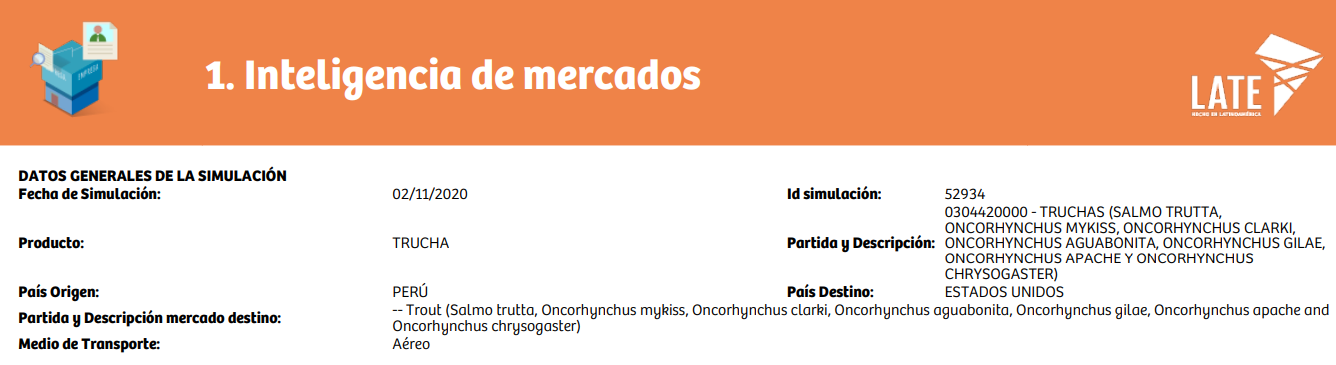
\includegraphics[keepaspectratio]{index_files/figure-html/lu137401d6rd_tmp_d9f9220d.png}}

}

\end{figure}%%
\begin{figure}[H]

\caption{Determinación de costos y el precio de exportación mediante el
simulador financiero LATE.}

{\centering \pandocbounded{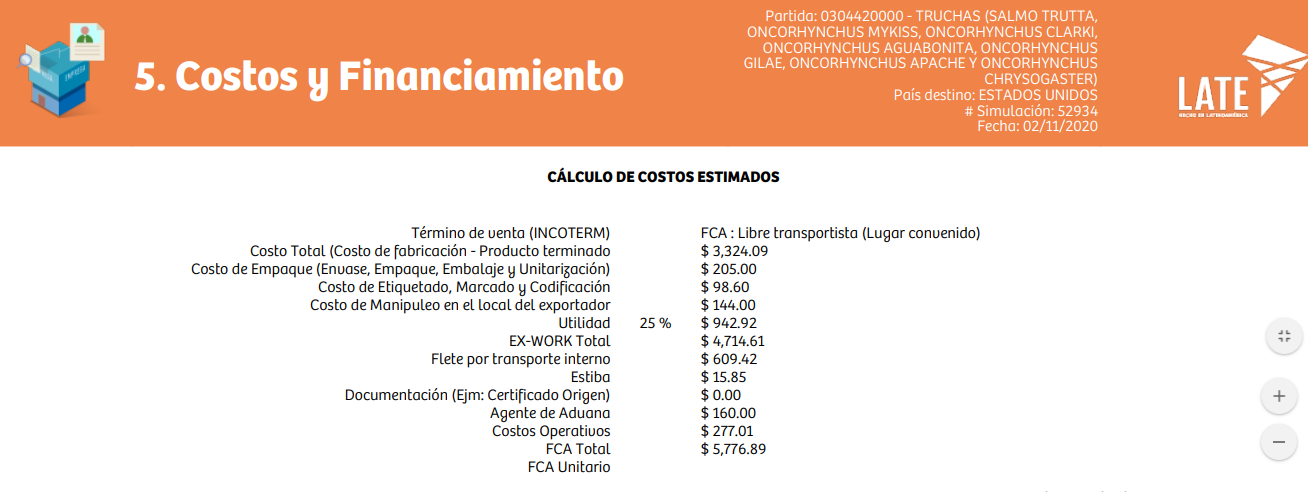
\includegraphics[keepaspectratio]{index_files/figure-html/lu137401d6rd_tmp_bd7c7d98.png}}

}

\end{figure}%

Acuicultura: alta conversión de alimento a carne. (2013, 13 de abril).
La Nación. Obtenido de
http://www.lanacion.com.ar/1571887-acuicultura-alta-conversion-de-alimento-a-carne

Agencia Agraria de Noticias. (2017a, 14 de junio). Perú y Chile
impulsarán pesca y acuicultura con sanidad e inocuidad. 2017. Obtenido
de
http://agraria.pe/noticias/peru-y-chile-impulsaran-pesca-y-acuicultura-con-sanidad-14084

Comisión de Promoción del Perú para la Exportación y el Turismo (2020).
\emph{Herramientas para las MIPYME: Simulador Financiero}. Consultado el
1 de noviembre de 2020. https://simuladorfinanciero.promperu.gob.pe/

Comisión de Promoción del Perú para la Exportación y el Turismo (2020).
\emph{Plataforma de exportación asistida LATE}. Obtenido de
https://www.late.gob.pe/Formularios/PasosFuncionales/frmInteligenciaMercado.aspx\#no-back-button

DP WORL Callao (2019). \emph{Tarifario de importación y exportación.}
Obtenido de
https://www.dpworldcallao.com.pe/uploads/tarifario/tarifario-abreviado-2019-1.pdf

Santander,Trade Markets. (s.f.). \emph{Estados Unidos, Política y
Economía}. Obtenido de
https://santandertrade.com/es/portal/analizar-mercados/estados-unidos/politica-y-economia

Sistema Integrado de Información de Comercio Exterior (2020).
\emph{Herramientas para las MIPYME: Calculador Callao Online.} Obtenido
de http://www.callaoonline.com/Cotizador.aspx

Sistema Integrado de Información de Comercio Exterior (2020).
\emph{Herramientas para las MIPYME: Tarifas de importación y exportación
Callao.} Obtenido de
https://www.neptunia.com.pe/HTML\_Libre/TARIFARIO\_WEB\_CAL.HTM

Plataforma de exportación asistida LATE (2020). \emph{Rutas aéreas}.
Obtenido de
\href{http://rutasaereas.promperu.gob.pe/}{http://rutasaereas.promperu.gob.pe/\#}

Velazco, J. (2019). \emph{Plan de exportación de filete de trucha
arcoíris hacia el mercado estadounidense} {[}tesis para optar el título
profesional, Universidad Nacional de Piura{]}. Repositorio Dspace
http://repositorio.unp.edu.pe/bitstream/handle/UNP/1681/ADM-VEL-GUT-2018.pdf?sequence=1\&isAllowed=y

CENTRAL INTELLIGENCE AGENCY. (2020). \emph{CENTRAL INTELLIGENCE AGENCY.
CENTRAL INTELLIGENCE}: Obtenido de
https://www.cia.gov/library/publications/the-world-factbook/

Ministerio de Comercio Exterior y Turismo. (2020). \emph{Informes y
Publicaciones}: Obtenido de https://www.gob.pe/mincetur

Ministerio de la Producción. (2020). \emph{Informes y Publicaciones}:
Obtenido de https://www.gob.pe/produce

U.S. FOOD \& DRUG. (2020). \emph{U.S. FOOD \& DRUG}. Obtenido de
Información para Consumidores ¨Consejos utiles para los consumidores de
la FDA¨: https://www.fda.gov/about-fda/fda-en-espanol

\section{Publicaciones Similares}\label{publicaciones-similares}

Si te interesó este artículo, te recomendamos que explores otros blogs y
recursos relacionados que pueden ampliar tus conocimientos. Aquí te dejo
algunas sugerencias:

\begin{enumerate}
\def\labelenumi{\arabic{enumi}.}
\tightlist
\item
  \href{https://achalmaedison.netlify.app/blog/posts/2015-05-14-el-aborto}{El
  Aborto} Lee sin conexión
  \href{https://achalmaedison.netlify.app/blog/posts/2015-05-14-el-aborto/index.pdf}{PDF}
\item
  \href{https://achalmaedison.netlify.app/blog/posts/2017-04-23-sitios-web-asombrosos}{Sitios
  Web Asombrosos} Lee sin conexión
  \href{https://achalmaedison.netlify.app/blog/posts/2017-04-23-sitios-web-asombrosos/index.pdf}{PDF}
\item
  \href{https://achalmaedison.netlify.app/blog/posts/2017-05-23-el-mercantilismo}{El
  Mercantilismo} Lee sin conexión
  \href{https://achalmaedison.netlify.app/blog/posts/2017-05-23-el-mercantilismo/index.pdf}{PDF}
\item
  \href{https://achalmaedison.netlify.app/blog/posts/2020-05-23-comandos-de-google-assistant}{Comandos
  De Google Assistant} Lee sin conexión
  \href{https://achalmaedison.netlify.app/blog/posts/2020-05-23-comandos-de-google-assistant/index.pdf}{PDF}
\item
  \href{https://achalmaedison.netlify.app/blog/posts/2020-09-15-plan-de-negocio-exportacion-de-trucha-arcoires}{Plan
  De Negocio Exportacion De Trucha Arcoires} Lee sin conexión
  \href{https://achalmaedison.netlify.app/blog/posts/2020-09-15-plan-de-negocio-exportacion-de-trucha-arcoires/index.pdf}{PDF}
\item
  \href{https://achalmaedison.netlify.app/blog/posts/2021-07-13-plan-de-negocio-exportacion-de-tuna}{Plan
  De Negocio Exportacion De Tuna} Lee sin conexión
  \href{https://achalmaedison.netlify.app/blog/posts/2021-07-13-plan-de-negocio-exportacion-de-tuna/index.pdf}{PDF}
\item
  \href{https://achalmaedison.netlify.app/blog/posts/2021-07-14-comandos-de-blogdown}{Comandos
  De Blogdown} Lee sin conexión
  \href{https://achalmaedison.netlify.app/blog/posts/2021-07-14-comandos-de-blogdown/index.pdf}{PDF}
\item
  \href{https://achalmaedison.netlify.app/blog/posts/2021-10-01-gestion-publica-y-administracion-publica}{Gestion
  Publica Y Administracion Publica} Lee sin conexión
  \href{https://achalmaedison.netlify.app/blog/posts/2021-10-01-gestion-publica-y-administracion-publica/index.pdf}{PDF}
\item
  \href{https://achalmaedison.netlify.app/blog/posts/2021-10-01-reformas-y-modernizacion-de-la-gestion-publica}{Reformas
  Y Modernizacion De La Gestion Publica} Lee sin conexión
  \href{https://achalmaedison.netlify.app/blog/posts/2021-10-01-reformas-y-modernizacion-de-la-gestion-publica/index.pdf}{PDF}
\item
  \href{https://achalmaedison.netlify.app/blog/posts/2022-04-22-economia-agraria}{Economia
  Agraria} Lee sin conexión
  \href{https://achalmaedison.netlify.app/blog/posts/2022-04-22-economia-agraria/index.pdf}{PDF}
\item
  \href{https://achalmaedison.netlify.app/blog/posts/2022-06-02-impacto-del-cambio-climatico}{Impacto
  Del Cambio Climatico} Lee sin conexión
  \href{https://achalmaedison.netlify.app/blog/posts/2022-06-02-impacto-del-cambio-climatico/index.pdf}{PDF}
\item
  \href{https://achalmaedison.netlify.app/blog/posts/2023-05-11-cualidades-de-los-servidores-publicos}{Cualidades
  De Los Servidores Publicos} Lee sin conexión
  \href{https://achalmaedison.netlify.app/blog/posts/2023-05-11-cualidades-de-los-servidores-publicos/index.pdf}{PDF}
\item
  \href{https://achalmaedison.netlify.app/blog/posts/2023-05-12-la-economia-peruana-entre-1970-1990}{La
  Economia Peruana Entre 1970 1990} Lee sin conexión
  \href{https://achalmaedison.netlify.app/blog/posts/2023-05-12-la-economia-peruana-entre-1970-1990/index.pdf}{PDF}
\item
  \href{https://achalmaedison.netlify.app/blog/posts/2023-05-16-economia-regional}{Economia
  Regional} Lee sin conexión
  \href{https://achalmaedison.netlify.app/blog/posts/2023-05-16-economia-regional/index.pdf}{PDF}
\end{enumerate}

Esperamos que encuentres estas publicaciones igualmente interesantes y
útiles. ¡Disfruta de la lectura!






\end{document}
